\setlength{\parskip}{0pt}
\linespread{0.9}
   
\usepackage[hyperindex]{hyperref}
\usepackage{bookmark}
\usepackage{enumitem}
\usepackage{xcolor}
\usepackage{ifthen}
\usepackage{bigfoot}
\usepackage{ragged2e}
\usepackage{needspace}
\usepackage[utf8x]{inputenc}
\usepackage[french]{babel}
\usepackage[protrusion=true,final]{microtype}
   
\usepackage{fontspec}
\usepackage{graphicx}
\usepackage{lettrine}
\renewcommand{\LettrineFontHook}{\lettrinefont}
\usepackage{titlesec}
\usepackage{titling}
\usepackage{fourier-orns}
\defaultfontfeatures{Ligatures=TeX}
\setmainfont{EB Garamond}

\makeatletter
 \newcommand{\linkdest}[1]{\Hy@raisedlink{\hypertarget{#1}{}}}
\makeatother

\newcommand{\negphantom}[1]{\settowidth{\dimen0}{#1}\hspace*{-\dimen0}}
\newcommand{\versenb}[1]{\par \vspace{10pt}~\linkdest{#1}\negphantom{~${}^{#1}$~}{}^{#1}$~}
\newcommand{\argument}[2]{\linkdest{arg-#1}#2}
\newcommand{\latin}[1]{\emph{#1}}

\usepackage{titlesec}
\usepackage[extramarks]{titleps}
\newfontfamily\secheadfont{EB Garamond}
\newcommand{\secheadstyle}{\secheadfont\large\textsc}
\titleformat{\section}[block]
  {}
  {}{0pt}
  {\secheadstyle}

\newcommand{\chapheadstyle}{\chapsecheadfont\Large\textsc}
\titleformat{\chapter}[block]
  {}
  {}{0pt}
  {\chapheadstyle}

\graphicspath{{images}} 
\title{PRÉPARATION AU RÈGNE DE JÉSUS-CHRIST}
%\title{TRAITÉ DE LA VRAIE DÉVOTION À LA SAINTE VIERGE}
\author{Saint Louis-Marie Grignion de Montfort, ca. 1713}
\begin{document}
\pagestyle{empty}
\resizebox{!}{0.9\pageheight}{
  \hspace{0pt}
  \vfill
  \begin{center}
    \begin{minipage}{0.7\textwidth}
      \begin{center}
        {\headerfont\Huge \thetitle} \\
        \vspace{0.1\pageheight}
        {\headerfont\Large \theauthor}
      \end{center}
    \end{minipage}
    \\
    \vspace{0.1\pageheight}
    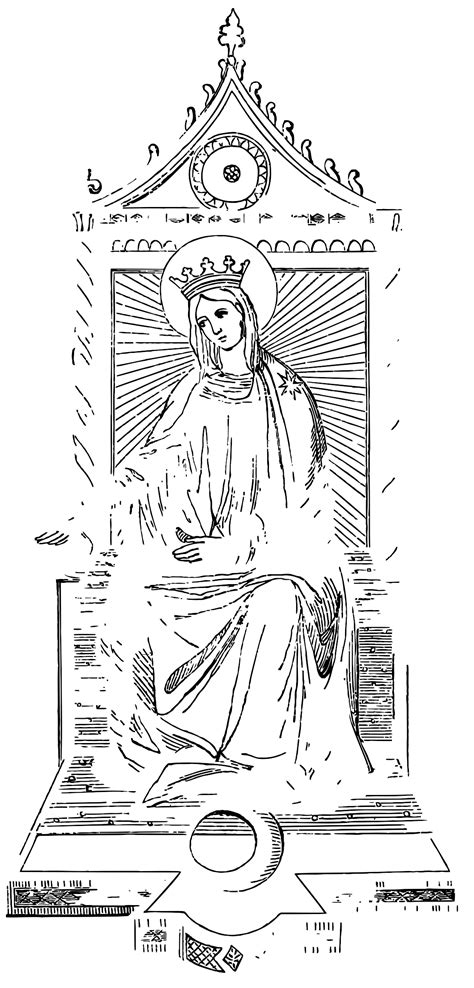
\includegraphics[height=0.4\pageheight]{th.jpg}
  \end{center}
  \vfill
}
\hspace{0pt}
\newpage
%\chapter{PRÉPARATION AU RÈGNE DE JÉSUS-CHRIST}
\section{I. NÉCESSITÉ QUE NOUS AVONS DE LA DÉVOTION À LA TRÈS-SAINTE VIERGE}
\subsection{A. NÉCESSITÉ DE LA DÉVOTION À MARIE}
\versenb{1} C'est par la Très Sainte Vierge Marie que Jésus-Christ est venu au monde, et c'est aussi par elle qu'il doit
régner dans le monde.
\versenb{2} Marie a été très cachée dans sa vie: c'est pour quoi elle est appelée par le Saint-Esprit et l'Eglise \latin{Alma Mater}:
Mère cachée et secrète. Son humilité a été si profonde qu'elle n'a point eu sur la terre d'attrait plus puissant et plus
continuel que de se cacher à elle-même et à toute créature, pour n'être connue que de Dieu seul.
\versenb{3} Dieu, pour l'exaucer dans les demandes qu'elle lui fit de la cacher, appauvrir et humilier, a pris plaisir à la
cacher dans sa conception, dans sa naissance, dans sa vie, dans ses mystères, dans sa résurrection et
assomption, à l'égard de presque toute créature humaine. Ses parents mêmes ne la connaissaient pas; et les
anges se demandaient souvent les uns aux autres: \latin{Quae est ista?} Qui est celle-là? Parce que le Très-Haut la leur
cachait; ou, s'il leur en découvrait quelque chose, il leur en cachait infiniment davantage.
\versenb{4} Dieu le Père a consenti qu'elle ne fît point de miracle dans sa vie, du moins qui éclatât, quoiqu'il lui en eût
donné la puissance. Dieu le Fils a consenti qu'elle ne parlât presque point, quoiqu'il lui eût communiqué sa
sagesse. Dieu le Saint-Esprit a consenti que ses Apôtres et ses Évangélistes n'en parlassent que très peu et
qu'autant qu'il était nécessaire pour faire connaître Jésus-Christ, quoiqu'elle fût son Épouse fidèle.
\versenb{5} Marie est l'excellent chef-d'oeuvre du Très-Haut, dont il s'est réservé la connaissance et la possession. Marie
est la Mère admirable du Fils, qu'il a pris plaisir à humilier et à cacher pendant sa vie, pour favoriser son humilité,
la traitant du nom de femme, mulier, comme une étrangère, quoique dans son coeur il l'estimât et l'aimât plus que
tous les anges et les hommes. Marie est la fontaine scellée et l'Épouse fidèle du Saint-Esprit, où il n'y a que lui qui
entre. Marie est le sanctuaire et le repos de la Sainte-Trinité, où Dieu est plus magnifiquement et divinement qu'en
aucun lieu de l'univers, sans excepter sa demeure sur les chérubins et les séraphins; et il n'est pas permis à
aucune créature, quelque pure qu'elle soit, d'y entrer sans un grand privilège.
\versenb{6} Je dis avec les saints: La divine Marie est le paradis terrestre du nouvel Adam, où il s'est incarné par l'opération
du Saint-Esprit, pour y opérer des merveilles incompréhensibles. C'est le grand et le divin monde de Dieu, où il y a
des beautés et des trésors ineffables. C'est la magnificence du Très-Haut où il a caché, comme en son sein, son
Fils unique, et en lui tout ce qu'il a de plus excellent et de plus précieux. Oh ! oh ! que de choses grandes et
cachées ce Dieu puissant a faites en cette créature admirable, comme elle est elle-même obligée de le dire,
malgré son humilité profonde: \latin{Fecit mihi magna qui potens est.} Le monde ne les connaît pas, parce qu'il en est
incapable et indigne.
\versenb{7} Les saints ont dit des choses admirables de cette sainte cité de Dieu; et ils n'ont jamais été plus éloquents et
plus contents, comme ils l'avouent eux-mêmes, que quand ils en ont parlé. Après cela, ils s'écrient que la hauteur
de ses mérites, qu'elle a élevés jusqu'au trône de la Divinité, ne se peut apercevoir; que la largeur de sa charité,
qu'elle a plus étendue que la terre, ne se peut mesurer; que la grandeur de sa puissance, qu'elle a jusque sur un
Dieu même, ne se peut comprendre; et, enfin, que la profondeur de son humilité et de toutes ses vertus et ses
grâces, qui sont un abîme, ne se peut sonder. O hauteur incompréhensible! O largeur ineffable! O grandeur
démesurée! O abîme impénétrable!
\versenb{8} Tous les jours, d'un bout de la terre à l'autre, dans le plus haut des cieux, dans le plus profond des abîmes, tout
prêche, tout publie l'admirable Marie. Les neuf choeurs des anges, les hommes de tous sexes, âges, conditions,
religions, bons et mauvais, jusqu'aux diables, sont obligés de l'appeler bienheureuse, bon gré, mal gré, par la force
de là vérité. Tous les anges dans les cieux lui crient incessamment, comme dit saint Bonaventure: \latin{Sancta, sancta,
sancta Maria, Dei Genitrix et Virgo}; et lui offrent millions de millions de fois tous les jours la Salutation des anges:
Ave, Maria, etc., en se prosternant devant elle, et lui demandant pour grâce de les honorer de quelques-uns de
ses commandements. Jusqu'à saint Michel [qui], dit saint Augustin, quoique le prince de toute la cour céleste, est
le plus zélé à lui rendre et à lui faire rendre toutes sortes d'honneurs, toujours en attente pour avoir l'honneur
d'aller, à sa parole, rendre service à quelqu'un de ses serviteurs.
\versenb{9} Toute la terre est pleine de sa gloire, particulièrement chez les chrétiens, où elle est prise pour tutélaire et
protectrice en plusieurs royaumes, provinces, diocèses et villes. Plusieurs cathédrales consacrées à Dieu sous son
nom. Point d'église sans autel en son honneur: point de contrée ni canton où il n'y ait quelqu'une de ses images
miraculeuses, où toutes sortes de maux sont guéris et toutes sortes de biens obtenus. Tant de confréries et
congrégations en son honneur ! tant de religions sous son nom et sa protection ! tant de confrères et soeurs de
toutes les confréries, et tant de religieux et religieuses de toutes les religions qui publient ses louanges et qui
annoncent ses miséricordes! Il n'y a pas un petit enfant qui, en bégayant l'Ave Maria, ne la loue; il n'y a guère de
pécheurs qui, en leur endurcissement même, n'aient en elle quelque étincelle de confiance; il n'y a pas même de
diable dans les enfers qui, en la craignant, ne la respecte.
\versenb{10} Après cela, il faut dire, en vérité, avec les saints:
\latin{De Maria numquam satis.}
On n'a point encore assez loué, exalté, honoré, aimé et servi Marie. Elle mérite encore plus de louanges, de
respects, d'amours et de services.
\versenb{11} Après cela, il faut dire avec le Saint-Esprit: \latin{Omnis gloria ejus filiae Regis ab intus}: Toute la gloire de la fille du
Roi est au-dedans: comme si toute la gloire extérieure que lui rendent à l'envi le ciel et la terre n'était rien, en
comparaison de celle qu'elle reçoit au-dedans par le Créateur, et qui n'est point connue des petites créatures, qui
ne peuvent pénétrer le secret des secrets du Roi.
\versenb{12} Après cela, il faut nous écrier avec l'Apôtre: \latin{Nec oculus vidit, nec auris audivit, nec in cor hominis ascendit}: Ni
l'oeil n'a vu, ni l'oreille n'a entendu, ni le coeur de l'homme n'a compris les beautés, les grandeurs et excellences
de Marie, le miracle des miracles de la grâce, de la nature et de la gloire. Si vous voulez comprendre la Mère, dit
un saint, comprenez le Fils. C'est une digne Mère de Dieu: \latin{Hic taceat omnis lingua}: Que toute langue demeure
muette ici.
\versenb{13} Mon coeur vient de dicter tout ce que je viens d'écrire, avec une joie particulière, pour montrer que la divine
Marie a été inconnue jusques ici, et que c'est une des raisons pourquoi Jésus-Christ n'est point connu comme il
doit être. Si donc, comme il est certain, la connaissance et le règne de Jésus-Christ arrivent dans le monde, ce ne
sera qu'une suite nécessaire de la connaissance et du règne de la Très Sainte Vierge Marie, qui l'a mis au monde
la première fois et le fera éclater la seconde.

\subsubsection{1- Dieu a voulu commencer et achever ses plus grands ouvrages par la très Sainte vierge}

\versenb{14} J'avoue, avec toute l'Église, que Marie n'étant qu'une pure créature sortie des mains du Très-Haut, comparée
à sa Majesté infinie, est moindre qu'un atome, ou plutôt n'est rien du tout, puisqu'il est seul «Celui qui est», et que,
par conséquent, ce grand Seigneur, toujours indépendant et suffisant à lui-même, n'a pas eu ni n'a pas encore
absolument besoin de la Très Sainte Vierge pour l'accomplissement de ses volontés et pour la manifestation de sa
gloire. Il n'a qu'à vouloir pour tout faire.
\versenb{15} \argument{constance}{Je dis cependant que, les choses supposées comme elles sont, Dieu ayant voulu commencer et achever ses
plus grands ouvrages par la Très Sainte Vierge depuis qu'il l'a formée, il est à croire qu'il ne changera point de
conduite dans les siècles des siècles, car il est Dieu, et ne change point en ses sentiments ni en sa conduite.}
\versenb{16} \argument{seule-digne}{Dieu le Père n'a donné son Unique au monde que par Marie. Quelques soupirs qu'aient poussés les
patriarches, quelques demandes qu'aient faites les prophètes et les saints de l'ancienne loi, pendant quatre mille
ans, pour avoir ce trésor, il n'y eut que Marie qui l'ait mérité et trouvé grâce devant Dieu par la force de ses prières
et la hauteur de ses vertus. Le monde étant indigne, dit saint Augustin, de (le) recevoir le Fils de Dieu
immédiatement des mains du Père, il l'a donné à Marie afin que le monde le reçût par elle.
Le Fils de Dieu s'est fait homme pour notre salut, mais en Marie et par Marie.}
Dieu le Saint-Esprit a formé Jésus-Christ en Marie, mais après lui avoir demandé son consentement par un des
premiers ministres de sa cour.
\versenb{17} \argument{fecondité}{Dieu le Père a communiqué à Marie sa fécondité autant qu'une pure créature en était capable, pour lui donner
le pouvoir de produire son Fils et tous les membres de son Corps mystique.}
\versenb{18} Dieu le Fils est descendu dans son sein virginal, comme le nouvel Adam dans son paradis terrestre, pour y
prendre ses complaisances et pour y opérer en cachette des merveilles de grâce. Ce Dieu fait homme a trouvé sa
liberté à se voir emprisonné dans son sein; il a fait éclater sa force à se laisser porter par cette petite fille; il a
trouvé sa gloire et celle de son Père à cacher ses splendeurs à toutes créatures d'ici-bas, pour ne les révéler qu'à
Marie; il a glorifié son indépendance et sa majesté à dépendre de cette aimable Vierge dans sa conception, en sa
naissance, en sa présentation au temple, en sa vie cachée de trente ans, jusqu'en sa mort, où elle devait assister,
pour ne faire avec elle qu'un même sacrifice, et pour être immolé par son consentement au Père éternel, comme
autrefois Isaac par le consentement d'Abraham à la volonté de Dieu. C'est elle qui l'a allaité, nourri, entretenu,
élevé et sacrifié pour nous.
O admirable et incompréhensible dépendance d'un Dieu que le Saint-Esprit n'a pu passer sous silence dans
l'Évangile, quoiqu'il nous ait caché presque toutes les choses admirables que cette Sagesse incarnée a faites dans
sa vie cachée --, pour nous en montrer le prix et la gloire infinie. Jésus-Christ a plus donné de gloire à Dieu son
Père par la soumission qu'il a eue à sa Mère pendant trente années, qu'il ne lui en eût donné en convertissant
toute la terre par l'opération des plus grandes merveilles. Oh! qu'on glorifie hautement Dieu quand on se soumet,
pour lui plaire, à Marie, à l'exemple de Jésus-Christ, notre unique modèle!
\versenb{19} Si nous examinons de près le reste de la vie de Jésus Christ, nous verrons qu'il a voulu commencer ses
miracles par Marie. Il a sanctifié saint Jean dans le sein de sa mère sainte Élisabeth, par la parole de Marie;
aussitôt qu'elle eût parlé, Jean fut sanctifié, et c'est son premier et plus grand miracle de grâce. Il changea, aux
noces de Cana, l'eau en vin, à son humble prière, et c'est son premier miracle de nature. Il a commencé et
continué ses miracles par Marie; et il les continuera jusques à la fin des siècles par Marie.
\versenb{20} Dieu le Saint-Esprit étant stérile en Dieu, c'est-à-dire ne produisant point d'autre personne divine, est devenu
fécond par Marie qu'il a épousée. C'est avec elle et en elle et d'elle qu'il a produit son chef-d'oeuvre, qui est un
Dieu fait homme, et qu'il produit tous les jours jusqu'à la fin du monde les prédestinés et les membres du corps de
ce chef adorable: c'est pourquoi plus il trouve Marie, sa chère et indissoluble Épouse, dans une âme, et plus il
devient opérant et puissant pour produire Jésus-Christ en cette âme et cette âme en Jésus-Christ.
\versenb{21} Ce n'est pas qu'on veuille dire que la Très Sainte Vierge donne au Saint-Esprit la fécondité, comme s'il ne
l'avait pas, puisque, étant Dieu, il a la fécondité ou la capacité de produire, comme le Père et le Fils, quoiqu'il ne la
réduise pas à l'acte, ne produisant point d'autre Personne divine. Mais on veut dire que le Saint-Esprit, par
l'entremise de la Sainte Vierge, dont il veut bien se servir, quoiqu'il n'en ait pas absolument besoin, réduit à l'acte
sa fécondité, en produisant en elle et par elle Jésus-Christ et ses membres. Mystère de grâce inconnu même aux
plus savants et spirituels d'entre les chrétiens.
\versenb{22} La conduite que les trois Personnes de la Très Sainte Trinité ont tenue dans l'Incarnation et le premier
avènement de Jésus-Christ, elles la gardent tous les jours, d'une manière invisible, dans la Sainte Église, et la
garderont jusqu'à la consommation des siècles, dans le dernier avènement de Jésus-Christ.
\versenb{23} Dieu le Père a fait un assemblage de toutes les eaux, qu'il a nommé la mer; il a fait un assemblage de toutes
ses grâces, qu'il a appelé Marie. Ce grand Dieu a un trésor ou un magasin très riche, où il a renfermé tout ce qu'il
a de beau, d'éclatant, de rare et de pré cieux, jusqu'à son propre Fils; et ce trésor immense n'est autre que Marie,
que les saints appellent le trésor du Seigneur, de la plénitude duquel les hommes sont enrichis.
\versenb{24} Dieu le Fils a communiqué à sa Mère tout ce qu'il a acquis par sa vie et sa mort, ses mérites infinis et ses
vertus admirables, et il l'a faite la trésorière de tout ce que son Père lui a donné en héritage; c'est par elle qu'il
applique ses mérites à ses membres, qu'il communique ses vertus et distribue ses grâces; c'est son canal
mystérieux, c'est son aqueduc, par où il fait passer doucement et abondamment ses miséricordes.
\versenb{25} Dieu le Saint-Esprit a communiqué à Marie, sa fidèle Épouse, ses dons ineffables, et il l'a choisie pour la
dispensatrice de tout ce qu'il possède: en sorte qu'elle distribue à qui elle veut, autant qu'elle veut, comme elle
veut et quand elle veut, tous ses dons et ses grâces, et il ne se donne aucun don céleste aux hommes qu'il ne
passe par ses mains virginales. Car telle est la volonté de Dieu, qui a voulu que nous ayons tout [par] Marie; car
ainsi sera enrichie, élevée et honorée du Très-Haut celle qui s'est appauvrie, humiliée et cachée jusqu'au fond du
néant par sa pro fonde humilité, pendant toute sa vie. Voilà les sentiments de l'Église et des Saints Pères.
\versenb{26} Si je parlais à des esprits forts de ce temps, je prouverais tout ce que je dis simplement, plus au long, par la
Sainte Écriture, les Saints Pères, dont je rapporterais les passages latins, et par plusieurs solides raisons qu'on
pourra voir au long déduites par le R.P. Poiré en sa Triple Couronne de la Sainte Vierge. Mais comme je parle
particulièrement aux pauvres et aux simples qui, étant de bonne volonté et ayant plus de foi que le commun des
savants, croient plus simplement et avec plus de mérite, je me contente de leur déclarer simplement la vérité, sans
m'arrêter à leur citer tous les passages latins, qu'ils n'entendent pas, quoique je ne laisse pas d'en rapporter
quelques-uns, sans les rechercher beaucoup. Continuons.
\versenb{27} La grâce perfectionnant la nature, et la gloire perfectionnant la grâce, il est certain que Notre Seigneur est
encore dans le ciel aussi Fils de Marie qu'il l'était sur la terre, et que, par conséquent, il a conservé la soumission
et l'obéissance du plus parfait de tous les enfants à l'égard de la meilleure de toutes les mères. Mais il faut prendre
garde de concevoir en cette dépendance quelque abaissement ou imperfection en Jésus-Christ. Car Marie étant
infiniment au dessous de son Fils, qui est Dieu, ne lui commande pas comme une mère d'ici bas commanderait à
son enfant qui est au-dessous d'elle. Marie, étant toute transformée en Dieu par la grâce et la gloire qui transforme
tous les saints en lui, ne demande, ne veut ni ne fait rien qui soit contraire à l'éternelle et immuable volonté de
Dieu. Quand on lit donc, dans les écrits des saints Bernard, Bernardin, Bonaventure, etc., que dans le ciel et sur la
terre, tout, jusqu'à Dieu même, est soumis à la Très Sainte Vierge, ils veulent dire que l'autorité que Dieu a bien
voulu lui donner est si grande, qu'il semble qu'elle a la même puissance que Dieu, et que ses prières et demandes
sont si puissantes auprès de Dieu, qu'elles passent toujours pour des commandements auprès de sa Majesté, qui
ne résiste jamais à la prière de sa chère Mère, parce qu'elle est toujours humble et conforme à sa volonté.
Si Moïse, par la force de sa prière, arrêta la colère de Dieu sur les Israélites, d'une manière si puissante que ce
très haut et infiniment miséricordieux Seigneur, ne pouvant lui résister, lui dit qu'il le laissât se mettre en colère et
punir ce peuple rebelle, que devons-nous penser, à plus forte raison, de la prière de l'humble Marie, la digne Mère
de Dieu, qui est plus puissante auprès de sa Majesté que les prières et intercessions de tous les anges et les
saints du ciel et de la terre?
\versenb{28} Marie commande dans les cieux sur les anges et les bienheureux. Pour récompense de son humilité profonde,
Dieu lui a donné le pouvoir et la commission de remplir de saints les trônes vides dont les anges apostats sont
tombés par orgueil. Telle est la volonté du Très-Haut, qui exalte les humbles, que le Ciel, la terre et les enfers
plient, bon gré mal gré, aux commandements de l'humble Marie, qu'il a faite la souveraine du ciel et de la terre, la
générale de ses armées, la trésorière de ses trésors, la dispensatrice de ses grâces, l'ouvrière de ses grandes
merveilles, la réparatrice du genre humain, la médiatrice des hommes, l'exterminatrice des ennemis de Dieu et la
fidèle compagne de ses grandeurs et de ses triomphes.
\versenb{29} Dieu le Père se veut faire des enfants par Marie jusqu'à la consommation du monde, et il lui dit ces paroles: \latin{In Jacob inhabita}, demeurez en Jacob, c'est-à-dire faites votre demeure et résidence dans mes enfants et
prédestinés, figurés par Jacob, et non point dans les enfants du diable et les réprouvés, figurés par Esaü.
\versenb{30} Comme dans la génération naturelle et corporelle il y a un père et une mère, de même dans la génération
surnaturelle et spirituelle il y a un père qui est Dieu et une mère qui est Marie. Tous les vrais enfants de Dieu et
prédestinés ont Dieu pour père et Marie pour mère; et qui n'a pas Marie pour Mère n'a pas Dieu pour Père. C'est
pourquoi les réprouvés, comme les hérétiques, schismatiques, etc., qui haïssent ou regardent avec mépris ou
indifférence la Très Sainte Vierge, n'ont point Dieu pour père, quoiqu'ils s'en glorifient, parce qu'ils n'ont point Marie
pour mère: car, s'ils l'avaient pour mère, ils l'aimeraient et l'honoreraient comme un vrai et bon enfant aime
naturellement et honore sa mère qui lui a donné la vie.
Le signe le plus infaillible et le plus indubitable pour distinguer un hérétique, un homme de mauvaise doctrine, un
réprouvé, d'avec un prédestiné, c'est que l'hérétique et le réprouvé n'ont que du mépris ou de l'indifférence pour la
Très Sainte Vierge, tâchant, par leurs paroles et exemples, d'en diminuer le culte et l'amour, ouvertement ou en
cachette, quelquefois sous de beaux prétextes. Hélas! Dieu le Père n'a pas dit à Marie de faire sa demeure en
eux, parce qu'ils sont des Esaüs.
\versenb{31} Dieu le Fils veut se former et, pour ainsi dire, s'incarner tous les jours, par sa chère Mère, dans ses membres,
et il lui dit: \latin{In Israel hereditare}: Ayez Israël pour héritage. C'est comme s'il disait: Dieu mon Père m'a donné pour
héritage toutes les nations de la terre, tous les hommes bons et mauvais, prédestinés et réprouvés; je conduirai les
uns par la verge d'or et les autres par la verge de fer; je serai le père et l'avocat des uns, le juste vengeur des
autres, et le juge de tous; mais pour vous, ma chère Mère, vous n'aurez pour votre héritage et possession que les
prédestinés, figurés par Israël; et, comme leur bonne mère, vous les enfanterez, nourrirez, élèverez; et, comme
leur souveraine, vous les conduirez, gouvernerez et défendrez.
\versenb{32} «Un homme et un homme est né en elle», dit le Saint-Esprit: Homo et homo natus est in ea. Selon l'explication
de quelques Pères, le premier homme qui est né en Marie est l'Homme- Dieu, Jésus-Christ, le second est un
homme pur, enfant de Dieu et de Marie par adoption. Si Jésus-Christ, le chef des hommes, est né en elle, les
prédestinés, qui sont les membres de ce chef, doivent aussi naître en elle par une suite nécessaire. Une même
mère ne met pas au monde la tête ou le chef sans les membres, ni les membres, sans la tête; autrement, ce serait
un monstre de nature; de même, dans l'ordre de la grâce, le chef et les membres naissent d'une même mère; et si
un membre du corps mystique de Jésus-Christ, c'est-à-dire un prédestiné, naissait d'une autre mère que Marie qui
a produit le chef, ce ne serait pas un prédestiné, ni un membre de Jésus-Christ, mais un monstre dans l'ordre de la
grâce.
\versenb{33} De plus, Jésus étant à présent autant que jamais le fruit de Marie, comme le Ciel et la terre lui répètent mille et
mille fois tous les jours: Et béni est le fruit de votre ventre, Jésus, il est certain que Jésus-Christ est pour chaque
homme en particulier, qui le possède, aussi véritablement le fruit et l'oeuvre de Marie, que pour tout le monde en
général; en sorte que, si quelque fidèle a Jésus-Christ formé dans son coeur, il peut dire hardiment: Grand merci à
Marie, ce que je possède est son effet et son fruit, et sans elle je ne l'aurais pas; et on peut lui appliquer plus
véritablement que saint Paul ne se les applique, ces paroles: \latin{Quos iterum parturio, donec in vobis formetur
Christus}: J'enfante tous les jours les enfants de Dieu, jusqu'à ce que Jésus-Christ mon Fils ne soit formé en eux
dans la plénitude de son age. Saint Augustin se surpassant soi-même, et tout ce que je viens de dire, dit que tous
les prédestinés, pour être conformes à l'image du Fils de Dieu, sont en ce monde cachés dans le sein de la Très
Sainte Vierge, où ils sont gardés, nourris, entretenus et agrandis par cette bonne Mère, jusqu'à ce qu'elle ne les
enfante à la gloire, après la mort, qui est proprement le jour de leur naissance, comme l'Église appelle la mort des
justes. O mystère de grâce inconnu aux réprouvés, et peu connu des prédestinés!
\versenb{34} Dieu le Saint-Esprit veut se former en elle et par elle des élus et il lui dit: \latin{In electis meis mitte radices}. Jetez,
ma bien-aimée et mon Épouse, les racines de toutes vos vertus dans mes élus, afin qu'ils croissent de vertu en
vertu et de grâce en grâce. J'ai pris tant de complaisance en vous, lorsque vous viviez sur la terre dans la pratique
des plus sublimes vertus, que je désire encore vous trouver sur la terre, sans cesser d'être dans le ciel.
Reproduisez-vous pour cet effet dans mes élus: que je voie en eux avec complaisance les racines de votre foi
invincible, de votre humilité profonde, de votre mortification universelle, de votre oraison sublime, de votre charité
ardente, de votre espérance ferme et de toutes vos vertus. Vous êtes toujours mon Épouse aussi fidèle, aussi pure
et aussi féconde que jamais: que votre foi me donne des fidèles; que votre pureté me donne des vierges, que
votre fécondité me donne des élus et des temples.
\versenb{35} Quand Marie a jeté ses racines dans une âme, elle y produit des merveilles de grâce qu'elle seule peut
produire parce qu'elle est seule la Vierge féconde qui n'a jamais eu ni n'aura jamais sa semblable en pureté et en
fécondité.
Marie a produit, avec le Saint-Esprit la plus grande chose qui ait été et sera jamais, qui est un Dieu Homme, et elle
produira conséquemment les plus grandes choses qui seront dans les derniers temps. La formation et l'éducation
des grands saints qui seront sur la fin du monde lui est réservée; car il n'y a que cette Vierge singulière et
miraculeuse qui peut produire, en union du Saint-Esprit, les choses singulières et extraordinaires.
\versenb{36} Quand le Saint-Esprit, son Époux, l'a trouvée dans une âme, il y vole, il y entre pleinement, il se communique
à cette âme abondamment et autant qu'elle donne place à son Épouse; et une des grandes raisons pourquoi le
Saint-Esprit ne fait pas maintenant des merveilles éclatantes dans les âmes, c'est qu'il n'y trouve pas une assez
grande union avec sa fidèle et indissoluble Épouse. Je dis: indissoluble Épouse, car depuis que cet Amour
substantiel du Père et du Fils a épousé Marie pour produire Jésus-Christ, le chef des élus et Jésus-Christ dans les
élus, il ne l'a jamais répudiée, parce qu'elle a toujours été fidèle et féconde.
\subsubsection{2- La dévotion à la Très Sainte Vierge est nécessaire}
\versenb{37} On doit conclure évidemment de ce que je viens de dire:
Premièrement, que Marie a reçu de Dieu une grande domination dans les âmes des élus: car elle ne peut pas faire
en eux sa résidence, comme Dieu le Père lui a ordonné; les former, les nourrir et les enfanter à la vie éternelle
comme leur mère, les avoir pour son héritage et sa portion, les former en Jésus-Christ et Jésus-Christ en eux; jeter
dans leur coeur les racines de ses vertus, et être la compagne indissoluble du Saint-Esprit pour tous ces ouvrages
de grâce; elle ne peut pas, dis-je, faire toutes ces choses, qu'elle n'ait droit et domination dans leurs âmes par une
grâce singulière du Très-Haut, qui, lui ayant donné puissance sur son Fils unique et naturel, la lui a aussi donnée
sur ses enfants adoptifs, non seulement quant au corps, ce qui serait peu de chose, mais aussi quant à l'âme.
\versenb{38} Marie est la Reine du ciel et de la terre par grâce, comme Jésus en est le Roi par nature et par conquête . Or,
comme le royaume de Jésus-Christ consiste principalement dans le coeur ou l'intérieur de l'homme, selon cette
parole: Le royaume de Dieu est au-dedans de nous, de même le royaume de la Très Sainte Vierge est
principalement dans l'intérieur de l'homme, c'est-à-dire son âme, et c'est principalement dans les âmes qu'elle est
plus glorifiée avec son Fils que dans toutes les créatures visibles, et nous pouvons l'appeler avec les saints la
Reine des coeurs.
\versenb{39} Secondement, il faut conclure que la Très Sainte Vierge étant nécessaire à Dieu, d'une nécessité qu'on
appelle hypothétique, en conséquence de sa volonté, elle est bien plus nécessaire aux hommes pour arriver à leur
dernière fin. Il ne faut donc pas mêler la dévotion à la Très Sainte Vierge avec les dévotions aux autres saints,
comme si elle n'était pas plus nécessaire, et que de surérogation.
\versenb{40} Le docte et le pieux Suarez, de la Compagnie de Jésus, le savant et le dévot Juste-Lipse, docteur de Louvain,
et plusieurs autres, ont prouvé invinciblement, en conséquence des sentiments des Pères, entre autres de saint
Augustin, de saint Éphrem, diacre d'Édesse, de saint Cyrille de Jérusalem, de saint Germain de Constantinople,
de saint Jean de Damas, de saint Anselme, saint Bernard, saint Bernardin, saint Thomas et saint Bonaventure,
que la dévotion à la Très Sainte Vierge est nécessaire au salut , et que c'est une marque infaillible de réprobation,
au sentiment même d'Œcolampade et de quelques autres hérétiques, de n'avoir pas de l'estime et de l'amour pour
la Sainte Vierge, et qu'au contraire c'est une marque infaillible de prédestination de lui être entièrement et
véritablement dévoué ou dévot.
\versenb{41} Les figures et les paroles de l'Ancien et du Nouveau Testa ment le prouvent, les sentiments et les exemples
des saints le confirment, la raison et l'expérience l'apprennent et le démontrent; le diable même, et ses suppôts,
pressés par la force de la vérité, ont été souvent obligés de l'avouer malgré eux. De tous ces passages des saints
Pères et des Docteurs, dont j'ai fait un ample recueil pour prouver cette vérité, je n'en rapporte qu'un afin de n'être
pas trop long: \latin{Tibi devotum esse, est arma quaedam salutis quae Deus his dat quos vult salvos fieri} (S. Joan.
Damas): Vous être dévot, ô Sainte Vierge, dit saint Jean Damascène, est une arme de salut que Dieu donne à
ceux qu'il veut sauver.
\versenb{42} Je pourrais ici rapporter plusieurs histoires qui prouvent la même chose, entre autres: I° celle qui est rapportée
dans les chroniques de saint François, lorsqu'il vit dans une extase une grande échelle qui allait au ciel, au bout de
laquelle était la Sainte Vierge et par laquelle il lui fut montré qu'il fallait monter pour arriver au ciel; 2° celle qui est
rapportée dans les chroniques de saint Dominique 5, lorsque quinze mille démons possédant l'âme d'un
malheureux hérétique, près de Carcassonne, où saint Dominique prêchait le Rosaire, furent obligés, à leur
confusion, par le commandement que leur en fit la Sainte Vierge, d'avouer plusieurs grandes et consolantes
vérités touchant la dévotion à la Sainte Vierge, avec tant de force et de clarté, qu'on ne peut pas lire cette histoire
authentique et le panégyrique que le diable fit malgré lui de la dévotion à la Très Sainte Vierge, sans verser des
larmes de joie, pour peu qu'on soit dévot à la Très Sainte Vierge.
\versenb{43} Si la dévotion à la Très Sainte Vierge est nécessaire à tous les hommes pour faire simplement leur salut, elle
l'est encore beaucoup plus à ceux qui sont appelés à une perfection particulière; et je ne crois pas qu'une
personne puisse acquérir une union intime avec Notre-Seigneur et une parfaite fidélité au Saint-Esprit, sans une
très grande union avec la Très Sainte Vierge et une grande dépendance de son secours.
\versenb{44} C'est Marie seule qui a trouvé grâce devant Dieu, sans aide d'aucune autre pure créature. Ce n'est que par
elle que tous ceux qui ont trouvé grâce devant Dieu depuis elle l'ont trouvée, et ce n'est que par elle que tous ceux
qui viendront ci-après la trouveront. Elle était pleine de grâce quand elle fut saluée par l'archange Gabriel, elle fut
surabondamment remplie de grâce par le Saint-Esprit quand il la couvrit de son ombre ineffable; et elle a
[tellement] augmenté de jour en jour [et] de moment en moment cette plénitude double, qu'elle est arrivée à un
point de grâce immense et inconcevable; en sorte que le Très-Haut l'a faite l'unique trésorière de ses trésors et
l'unique dispensatrice de ses grâces, pour anoblir, élever et enrichir qui elle veut, pour faire entrer qui elle veut
dans la voie étroite du ciel, pour faire passer, malgré tout, qui elle veut par la porte étroite de la vie, et pour donner
le trône, le sceptre et la couronne de roi à qui elle veut. Jésus est partout et toujours le fruit et le Fils de Marie; et
Marie est partout l'arbre véritable qui porte le fruit de vie, et la vraie mère qui le produit.
\versenb{45} C'est Marie seule à qui Dieu a donné les clefs des celliers du divin amour, et le pouvoir d'entrer dans les voies
les plus sublimes et les plus secrètes de la perfection, et d'y faire entrer les autres. C'est Marie seule qui donne
l'entrée dans le paradis terrestre aux misérables enfants d'Eve l'infidèle, pour s'y promener agréablement avec
Dieu, pour s'y cacher sûrement contre ses ennemis et pour s'y nourrir délicieusement, et sans plus craindre la
mort, du fruit des arbres de vie et de science du bien et du mal et pour y boire à longs traits les eaux célestes de
cette belle fontaine qui y rejaillit avec abondance; ou plutôt comme elle est elle même ce paradis terrestre, ou cette
terre vierge et bénite dont Adam et Eve les pécheurs ont été chassés, elle ne donne entrée chez elle qu'à ceux et
celles qu'il lui plaît pour les faire devenir saints.
\versenb{46} Tous les riches du peuple, pour me servir de l'expression du Saint-Esprit, selon l'explication de saint Bernard,
tous les riches du peuple supplieront votre visage de siècle en siècle, et particulièrement à la fin du monde, c'est-àdire que les plus grands saints, les âmes les plus riches en grâce et en vertus, seront les plus assidus à prier la
Très Sainte Vierge et à l'avoir toujours présente comme leur parfait modèle pour l'imiter, et leur aide puissante
pour les secourir.
\versenb{47} J'ai dit que cela arriverait particulièrement à la fin du monde, et bientôt, parce que le Très-Haut avec sa sainte
Mère doivent se former de grands saints qui surpasseront autant en sainteté la plupart des autres saints, que les
cèdres du Liban surpassent les petits arbrisseaux, comme il a été révélé à une sainte âme, dont la vie a été écrite
par Mr. de Renty.
\versenb{48} Ces grandes âmes, pleines de grâce et de zèle, seront choisies pour s'opposer aux ennemis de Dieu, qui
frémiront de tous côtés, et elles seront singulière ment dévotes à la Très Sainte Vierge, éclairées par sa lumière,
nourries de son lait, conduites par son esprit, soutenues par son bras et gardées sous sa protection, en sorte
qu'elles combattront d'une main et édifieront de l'autre. D'une main, elles combattront, renverseront, écraseront les
hérétiques avec leurs hérésies, les schismatiques avec leurs schismes, les idolâtres avec leur idolatrie, et les
pécheurs avec leurs impiétés; et, de l'autre main, elles édifieront le temple du vrai Salomon et la mystique cité de
Dieu, c'est-à-dire la Très Sainte Vierge, appelée par les Saints Pères le temple de Salomon et la cité de Dieu. Ils
porteront tout le monde, par leurs paroles et leurs exemples, à sa véritable dévotion, ce qui leur attirera beaucoup
d'ennemis, mais aussi beaucoup de victoires et de gloire pour Dieu seul. C'est ce que Dieu a révélé à saint Vincent
Ferrier, grand apôtre de son siècle, comme il l'a suffisamment marqué dans un de ses ouvrages.
C'est ce que le Saint-Esprit semble avoir prédit dans le Psaume 58e, dont voici les paroles: \latin{Et scient quia Dominus
dominabitur Jacob et finium terrae; convertentur ad vesperam, et famem pati entur ut canes, et circuibunt
civitatem}: Le Seigneur régnera dans Jacob et dans toute la terre; ils se convertiront sur le soir, et ils souffriront la
faim comme des chiens, et ils iront autour de la ville pour trouver de quoi manger. Cette ville que les hommes
tournoieront à la fin du monde pour se convertir, et pour rassasier la faim qu'ils auront de la justice, est la Très
Sainte Vierge qui est appelée par le Saint-Esprit ville et cité de Dieu.
\subsection{B. Nécessité de la dévotion à Marie particulièrement dans les derniers temps}
\versenb{49} C'est par Marie que le salut du monde a commencé, et c'est par Marie qu'il doit être consommé. Marie n'a
presque point paru dans le premier avènement de Jésus-Christ, afin que les hommes, encore peu instruits et
éclairés sur la personne de son Fils, ne s'éloignassent de la vérité, en s'attachant trop fortement et trop
grossièrement à elle, ce qui apparemment serait arrivé si elle avait été connue, à cause des charmes admirables
que le Très-Haut avait mis même en son extérieur; ce qui est si vrai que saint Denis l'Aréopagite nous a laissé par
écrit que, quand il la vit, il l'aurait prise pour une divinité, à cause de ses charmes secrets et de sa beauté
incomparable, si la foi, dans laquelle il était bien confirmé, ne lui avait appris le con traire. Mais, dans le second
avènement de Jésus-Christ, Marie doit être connue et révélée par le Saint-Esprit afin de faire par elle connaître,
aimer et servir Jésus-Christ, les raisons qui ont porté le Saint-Esprit à cacher son Épouse pendant sa vie, et à ne
la révéler que bien peu depuis la prédication de l'Évangile, ne subsistant plus.
\subsubsection{1- Dieu veut révéler et découvrir Marie dans les derniers temps}}
\versenb{50} Dieu veut donc révéler et découvrir Marie, le chef-d'oeuvre de ses mains, dans ces derniers temps.
I° Parce qu'elle s'est cachée dans ce monde et s'est mise plus bas que la poussière par sa profonde humilité,
ayant obtenu de Dieu, de ses Apôtres et Évangélistes, qu'elle ne fût point manifestée.
2° Parce qu'étant le chef-d'oeuvre des mains de Dieu, aussi bien ici-bas par la grâce que dans le ciel par la gloire,
il veut en être glorifié et loué sur la terre par les vivants.
3° Comme elle est l'aurore qui précède et découvre le Soleil de justice, qui est Jésus-Christ, elle doit être connue
et aperçue, afin que Jésus-Christ le soit.
4° Étant la voie par laquelle Jésus-Christ est venu à nous la première fois, elle le sera encore lorsqu'il viendra la
seconde, quoique non pas de la même manière.
5° Étant le moyen sûr et la voie droite et immaculée pour aller à Jésus-Christ et le trouver parfaitement, c'est par
elle que les saintes âmes qui doivent éclater en sainteté doivent le trouver. Celui qui trouvera Marie trouvera la vie,
c'est-à-dire Jésus Christ, qui est la voie, la vérité et la vie. Mais on ne peut trouver Marie qu'on ne la cherche; on
ne peut la chercher qu'on ne la connaisse: car on ne cherche ni on ne désire un objet inconnu. Il faut donc que
Marie soit plus connue que jamais, à la plus grande connaissance et gloire de la Très Sainte Trinité.
6° Marie doit éclater, plus que jamais, en miséricorde, en force et en grâce dans ces derniers temps: en
miséricorde, pour ramener et recevoir amoureusement les pauvres pécheurs et dévoyés qui se converti ront et
reviendront à l'Église catholique; en force contre les ennemis de Dieu, les idolâtres, schismatiques, mahométans,
juifs et impies endurcis, qui se révolteront terri blement pour séduire et faire tomber, par promesses et menaces,
tous ceux qui leur seront contraires; et enfin elle doit éclater en grâce, pour animer et sou tenir les vaillants soldats
et fidèles serviteurs de Jésus-Christ qui combattront pour ses intérêts.
7° Enfin Marie doit être terrible au diable et à ses suppôts comme une armée rangée en bataille, principalement
dans ces derniers temps, parce que le diable, sachant bien qu'il a peu de temps, et beaucoup moins que jamais,
pour perdre les âmes, il redouble tous les jours ses efforts et ses combats; il suscitera bientôt de cruelles
persécutions, et mettra de terribles embûches aux serviteurs fidèles et aux vrais enfants de Marie, qu'il a plus de
peine à surmonter que les autres.
\versenb{51} C'est principalement de ces dernières et cruelles persécutions du diable qui augmenteront tous les jours
jusqu'au règne de l'Antéchrist, qu'on doit entendre cette première et célèbre prédiction et malédiction de Dieu,
portée dans le paradis terrestre contre le serpent. Il est à propos de l'expliquer ici pour la gloire de la Très Sainte
Vierge, le salut de ses enfants et la confusion du diable.
\latin{Inimicitias ponam inter te et mulierem, et semen tuum et semen illius; ipsa conteret caput tuum, et tu insidiaberis
calcaneo ejus} (Gen., III, I5): Je mettrai des inimitiés entre toi et la femme, et ta race et la sienne; elle-même
t'écrasera la tête, et tu mettras des embûches à son talon.
\versenb{52} Jamais Dieu n'a fait et formé qu'une inimitié, mais irréconciliable, qui durera et augmentera même jusques à la
fin: c'est entre Marie, sa digne Mère, et le diable, entre les enfants et serviteurs de la Sainte Vierge, et les enfants
et suppôts de Lucifer; en sorte que la plus terrible des ennemies que Dieu ait faite contre le diable est Marie, sa
sainte Mère. Il lui a même donné, dès le paradis terrestre, quoiqu'elle ne fût encore que dans son idée, tant de
haine contre ce maudit ennemi de Dieu, tant d'industrie pour découvrir la malice de cet ancien serpent, tant de
force pour vaincre, terrasser et écraser cet orgueilleux impie, qu'il l'appréhende plus, non seulement que tous les
anges et les hommes, mais, en un sens, que Dieu même. Ce n'est pas que l'ire, la haine et la puissance de Dieu
ne soient infiniment plus grandes que celles de la Sainte Vierge, puisque les perfections de Marie sont limitées;
mais c'est premièrement parce que Satan, étant orgueilleux, souffre infiniment plus d'être vaincu et puni par une
petite et humble servante de Dieu, et son humilité l'humilie plus que le pouvoir divin, secondement parce que Dieu
a donné à Marie un si grand pouvoir contre les diables, qu'ils craignent plus, comme ils ont été souvent obligés
d'avouer, malgré eux, par la bouche des possédés, un seul de ses soupirs pour quelque âme, que les prières de
tous les saints, et une seule de ses menaces contre eux que tous leurs autres tourments.
\versenb{53} Ce que Lucifer a perdu par orgueil, Marie l'a gagné par humilité; ce qu'Eve a damné et perdu par
désobéissance, Marie l'a sauvé par obéissance. Eve, en obéissant au serpent, a perdu tous ses enfants avec elle,
et les lui a livrés; Marie, s'étant rendue parfaitement fidèle à Dieu, a sauvé tous ses enfants et serviteurs avec elle,
et les a consacrés à sa Majesté .
\versenb{54} Non seulement Dieu a mis une inimitié, mais des inimitiés, non seulement entre Marie et le démon mais entre
la race de la Sainte Vierge et la race du démon; c'est-à-dire que Dieu a mis des inimitiés, des antipathies et haines
secrètes entre les vrais enfants et serviteurs de la Sainte Vierge et les enfants et esclaves du diable; ils ne
s'aiment point mutuellement, ils n'ont point de correspondance intérieure les uns avec les autres. Les enfants de
Bélial, les esclaves de Satan, les amis du monde (car c'est la même chose), ont toujours persécuté jusqu'ici et
persécuteront plus que jamais ceux et celles qui appartiennent à la Très Sainte Vierge, comme autrefois Caïn
persécuta son frère Abel, et Esaü son frère Jacob, qui sont les figures des réprouvés et des prédestinés. Mais
l'humble Marie aura toujours la victoire sur cet orgueilleux, et si grande qu'elle ira jusqu'à lui écraser la tête où
réside son orgueil; elle découvrira toujours sa malice de serpent; elle éventera ses mines infernales, elle dissipera
ses conseils diaboliques, et garantira jusqu'à la fin des temps ses fidèles serviteurs de sa patte cruelle.
Mais le pouvoir de Marie sur tous les diables éclatera particulièrement dans les derniers temps, où Satan mettra
des embûches à son talon, c'est-à-dire à ses humbles esclaves et à ses pauvres enfants qu'elle sus citera pour lui
faire la guerre. Ils seront petits et pauvres selon le monde, et abaissés devant tous comme le talon, foulés et
persécutés comme le talon l'est à l'égard des autres membres du corps; mais, en échange, ils seront riches en
grâce de Dieu, que Marie leur distribuera abondamment, grands et relevés en sainteté devant Dieu, supérieurs à
toute créature par leur zèle animé, et si fortement appuyés du secours divin, qu'avec l'humilité de leur talon, en
union de Marie, ils écraseront la tête du diable et feront triompher Jésus-Christ.
2. La dévotion à Marie nécessaire
particulièrement dans les derniers temps
\versenb{55} Enfin Dieu veut que sa sainte Mère soit à présent plus connue, plus aimée, plus honorée que jamais elle n'a
été: ce qui arrivera sans doute, si les prédestinés entrent, avec la grâce et lumière du Saint-Esprit, dans la pratique
intérieure et par faite que je leur découvrirai dans la suite. Pour lors, ils verront clairement, autant que la foi le
permet, cette belle étoile de la mer, et ils arriveront à bon port, malgré les tempêtes et les pirates, en suivant sa
conduite; ils connaîtront les grandeurs de cette souveraine, et ils se consacreront entièrement à son service,
comme ses sujets et ses esclaves d'amour; ils éprouveront ses douceurs et ses bontés maternelles, et ils
l'aimeront tendrement comme ses enfants bien-aimés; ils connaîtront les miséricordes dont elle est pleine et les
besoins où ils sont de son secours, et ils auront recours à e]le en toutes choses comme à leur chère avocate et
médiatrice auprès de Jésus-Christ; ils sauront qu'elle est le moyen le plus assuré, le plus aisé, le plus court et le
plus parfait pour aller à Jésus Christ, et ils se livreront à elle corps et âme, sans partage, pour être à Jésus-Christ
de même.
\versenb{56} Mais qui seront ces serviteurs, esclaves et enfants de Marie?
Ce seront un feu brûlant, ministres du Seigneur qui mettront le feu de l'amour divin partout.
Ce seront sicut sagittae in manum potentis, des flèches aiguës dans la main de la puissante Marie pour percer ses
ennemis.
Ce seront des enfants de Lévi, bien purifiés par le feu de grandes tribulations et bien collés à Dieu, qui porteront
l'or de l'amour dans le coeur, l'encens de l'oraison dans l'esprit et la myrrhe de la mortification dans le corps, et qui
seront part out la bonne odeur de Jésus-Christ aux pauvres et aux petits, tandis qu'ils seront une odeur de mort
aux grands, aux riches et orgueilleux mondains.
\versenb{57} Ce seront des nues tonnantes et volantes par les airs au moindre souffle du Saint-Esprit, qui, sans s'attacher à
rien, ni s'étonner de rien, ni se mettre en peine de rien, répandront la pluie de la parole de Dieu et de la vie
éternelle; ils tonneront contre le péché, ils gronderont contre le monde, ils frapperont le diable et ses suppôts, et ils
perceront d'outre en outre, pour la vie ou pour la mort, avec leur glaive à deux tranchants de la parole de Dieu,
tous ceux auxquels ils seront envoyés de la part du Très-Haut.
\versenb{58} Ce seront des apôtres véritables des derniers temps, à qui le Seigneur des vertus donnera la parole et la force
pour opérer des merveilles et remporter des dépouilles glorieuses sur ses ennemis; ils dormiront sans or ni argent
et, qui plus est, sans soin, au milieu des autres prêtres, et ecclésiastiques et clercs, inter medios cleros; et
cependant auront les ailes argentées de la colombe, pour aller avec la pure intention de la gloire de Dieu et du
salut des âmes, où le Saint-Esprit les appellera, et ils ne laisseront après eux, dans les lieux où ils auront prêché,
que l'or de la charité qui est l'accomplissement de toute la loi
\versenb{59} Enfin, nous savons que ce seront de vrais disciples de Jésus-Christ, qui marchant sur les traces de sa
pauvreté, humilité, mépris du monde et charité, enseignant la voie étroite de Dieu dans la pure vérité, selon le saint
Évangile, et non selon les maximes du monde, sans se mettre en peine ni faire acception de personne, sans
épargner, écouter ni craindre aucun mortel, quelque puissant qu'il soit. Ils auront dans leur bouche le glaive à deux
tranchants de la parole de Dieu; ils porteront sur leurs épaules l'étendard ensanglanté de la Croix, le crucifix dans
la main droite, le chapelet dans la gauche, les sacrés noms de Jésus et de Marie sur leur cœur, et la modestie et
mortification de Jésus-Christ dans toute leur conduite.
Voilà de grands hommes qui viendront, mais que Marie fera par ordre du Très-Haut, pour étendre son empire sur
celui des impies, idolâtres et mahométans. Mais quand et comment cela sera-t-il ?... Dieu seul le sait: c'est à nous
de nous taire, de prier, soupirer et attendre: Exspectans exspectavi.
\section{II. EN QUOI CONSISTE LA DÉVOTION À MARIE}
\subsection{A. Vérités fondamentales de la dévotion à la Sainte Vierge}
\versenb{60} Ayant jusqu'ici dit quelque chose de la nécessité que nous avons de la dévotion à la Très Sainte Vierge, il faut
dire en quoi consiste cette dévotion; ce que je ferai, Dieu aidant, après que j'aurai présupposé quelques vérités
fondamentales, qui donneront jour à cette grande et solide dévotion que je veux découvrir.
Jésus-Christ est la fin dernière de toutes nos dévotions
\versenb{61} Première vérité. Jésus-Christ notre Sauveur, vrai Dieu et vrai homme, doit être la fin dernière de toutes nos
autres dévotions; autrement elles seraient fausses et trompeuses. Jésus Christ est l'alpha et l'oméga, le
commencement et la fin de toutes choses. Nous ne travaillons, comme dit l'Apôtre, que pour rendre tout homme
parfait en Jésus-Christ, parce que c'est en lui seul qu'habite[nt] toute la plénitude de la Divinité et toutes les autres
plénitudes de grâces, de vertus et de perfections; parce que c'est en lui seul que nous avons été bénis de toute
bénédiction spirituelle; parce qu'il est notre unique maître qui doit nous enseigner, notre unique Seigneur de qui
nous devons dépendre, notre unique chef auquel nous devons être unis, notre unique modèle auquel nous devons
nous conformer, notre unique médecin qui doit nous guérir, notre unique pasteur qui doit nous nourrir, notre unique
voie qui doit nous conduire, notre unique vérité que nous devons croire, notre unique vie qui doit nous vivifier et
notre unique tout en toutes choses qui doit nous suffire. Il n'a point été donné d'autre nom sous le ciel, que le nom
de Jésus, par lequel nous devions être sauvés. Dieu ne nous a point mis d'autre fondement de notre salut, de
notre perfection et de notre gloire, que Jésus-Christ: tout édifice qui n'est pas posé sur cette pierre ferme est fondé
sur le sable mouvant, et tombera infailliblement tôt ou tard. Tout fidèle qui n'est pas uni à lui comme une branche
au cep de la vigne, tombera, séchera et ne sera propre qu'à être jeté au feu Si nous sommes en Jésus-Christ et
Jésus-Christ en nous, nous n'avons point de damnation à craindre; ni les anges des cieux, ni les hommes de la
terre, ni les démons des enfers, ni aucune autre créature ne nous peut nuire, parce qu'elle ne nous peut séparer
de la charité de Dieu qui est en Jésus-Christ. Par Jésus-Christ, avec Jésus-Christ, en Jésus-Christ, nous pouvons
toutes choses: rendre tout honneur et gloire au Père, en l'unité du Saint-Esprit; nous rendre parfaits et être à notre
prochain une bonne odeur de vie éternelle.
\versenb{62} Si donc nous établissons la solide dévotion de la Très Sainte Vierge, ce n'est que pour établir plus
parfaitement celle de Jésus-Christ, ce n'est que pour donner un moyen aisé et assuré pour trouver Jésus-Christ. Si
la dévotion à la Sainte Vierge éloignait de Jésus-Christ, il faudrait la rejeter comme une illusion du diable; mais tant
s'en faut qu'au contraire, comme j'ai déjà fait voir et ferai voir encore ci-après cette dévotion ne nous est
nécessaire que pour trouver Jésus-Christ parfaitement et l'aimer tendrement et le servir fidèlement.
\versenb{63} Je me tourne ici un moment vers vous, ô mon aimable Jésus, pour me plaindre amoureusement à votre divine
Majesté de ce que la plupart des chrétiens, même des plus savants, ne savent pas la liaison nécessaire, qui est
entre vous et votre sainte Mère. Vous êtes, Seigneur, toujours avec Marie, et Marie est toujours avec vous et ne
peut être sans vous: autrement elle cesserait d'être ce qu'elle est; elle est tellement transformée en vous par la
grâce qu'elle ne vit plus, qu'elle n'est plus; c'est vous seul, mon Jésus, qui vivez et régnez en elle, plus
parfaitement qu'en tous les anges et les bienheureux. Ah! si on connaissait la gloire et l'amour que vous recevez
en cette admirable créature, on aurait de vous et d'elle bien d'autres sentiments qu'on n'a pas. Elle [vous] est si
intimement unie, qu'on séparerait plutôt la lumière du soleil, la chaleur du feu; je dis plus, on séparerait plutôt tous
les anges et les saints de vous, que la divine Marie: parce qu'elle vous aime plus ardemment et vous glorifie plus
parfaitement que toutes vos autres créatures ensemble.
\versenb{64} Après cela, mon aimable Maître, n'est-ce pas une chose étonnante et pitoyable de voir l'ignorance et les
ténèbres de tous les hommes d'ici-bas à l'égard de votre sainte Mère? Je ne parle pas tant des idolâtres et païens,
qui, ne vous connaissant pas, n'ont garde de la connaître; je ne parle pas même des hérétiques et des
schismatiques, qui n'ont garde d'être dévots à votre sainte Mère, s'étant séparés de vous et de votre sainte Église;
mais je parle des chrétiens catholiques, et même des docteurs parmi les catholiques, qui faisant profession
d'enseigner aux autres les vérités, ne vous connaissent pas, ni votre sainte Mère, si ce n'est d'une manière
spéculative, sèche, stérile et indifférente . Ces messieurs ne parlent que rarement de votre sainte Mère et de la
dévotion qu'on lui doit avoir parce qu'ils craignent, disent-ils, qu'on en abuse, qu'on ne vous fasse injure en
honorant trop votre sainte Mère. S'ils voient ou entendent quelque dévot à la Sainte Vierge parler souvent de la
dévotion à cette bonne Mère, d'une manière tendre, forte et persuasive, comme d'un moyen assuré sans illusion,
d'un chemin court sans danger, d'une voie immaculée sans imperfection, et d'un secret merveilleux pour vous
trouver et vous aimer parfaitement, ils se récrient contre lui, et lui donnent mille fausses raisons pour lui prouver
qu'il ne faut pas qu'il parle tant de la Sainte Vierge, qu'il y a de grands abus en cette dévotion, et qu'il faut
s'appliquer à les détruire, et à parler de vous plutôt qu'à porter les peuples à la dévotion à la Sainte Vierge qu'ils
aiment déjà assez.
On les entend quelquefois parler de la dévotion à votre sainte Mère, non pas pour l'établir et la persuader, mais
pour en détruire les abus qu'on en fait, tandis que ces messieurs sont sans piété et sans dévotion tendre pour
vous, parce qu'ils n'en ont pas pour Marie, regardant le Rosaire, le Scapulaire, le Chapelet, comme des dévotions
de femmelettes, propres aux ignorants, sans lesquelles on peut se sauver; et s'il tombe en leurs mains quelque
dévot à la Sainte Vierge, qui récite son chapelet ou ait quelque autre pratique de dévotion envers elle, ils lui
changeront bientôt l'esprit et le coeur: au lieu du chapelet, ils lui conseilleront de dire les sept psaumes; au lieu de
la dévotion à la Jésus-Christ.
O mon aimable Jésus, ces gens ont-ils votre esprit? Vous font ils plaisir d'en agir de même ? Est-ce vous plaire
que de ne pas faire tous ses efforts pour plaire à votre Mère, de peur de vous déplaire? La dévotion à votre sainte
Mère empêche-t-elle la vôtre? Est-ce qu'elle s'attribue l'honneur qu'on lui rend? Est-ce qu'elle fait bande à part?
Est-elle une étrangère qui n'a aucune liaison avec vous? Est-ce vous déplaire que de vouloir lui plaire? Est-ce se
séparer ou s'éloigner de votre amour que de se donner à elle et de l'aimer ?
\versenb{65} Cependant, mon aimable Maître, la plupart des savants, pour punition de leur orgueil, n'éloigneraient pas plus
de la dévotion à votre sainte Mère, et n'en donneraient pas plus d'indifférence, que si tout ce que je viens de dire
était vrai. Gardez-moi, Seigneur, gardez-moi de leurs sentiments et leurs pratiques et me donnez quelque part aux
sentiments de reconnaissance, d'estime, de respect et d'amour que vous avez à l'égard de votre sainte Mère, afin
que je vous aime et glorifie d'autant plus que je vous imiterai et suivrai de plus près.
\versenb{66} Comme si jusqu'ici je n'avais encore rien dit en l'honneur de votre sainte Mère, faites-moi la grâce de la louer
dignement: \latin{Fac me digne tuam Matrem collaudare}, malgré tous ses ennemis, qui sont les vôtres, et que je leur
dise hautement avec les saints: \latin{Non presumat aliquis Deum se habere propitium qui benedictam Matrem offensam
habuerit}: Que celui-là ne présume pas recevoir la miséricorde de Dieu, qui offense sa sainte Mère.
\versenb{67} Pour obtenir de votre miséricorde une véritable dévotion à votre sainte Mère, et pour l'inspirer à toute la terre,
faites que je vous aime ardemment, et recevez pour cela la prière embrasée que je vous fais avec saint Augustin
et vos véritables amis (tom. 9, operum meditat.):
\latin{"Tu es Christus, pater meus sanctus, Deus meus pius, rex meus magnus, pastor meus bonus, magister meus
unus, adjutor meus opti mus, dilectus meus pulcherrimus, panis meus vivsus, sacerdos meus in aeternum, dux
meus ad patriam, Iux mea vera, dulcedo mea sanc ta, via mea recta, sapientia mea proeclara, simplicitas mea
pura, concordia mea pacifica, custodia mea tota, portio mea bona, salus mea sempiterna...
"Christe Jesu, amabilis Domine, cur amavi, quare concupivi in omni vita mea quidquam praeter te Jesum Deum
meum? Ubi eram quando tecum mente non eram? Jam ex hoc nunc, omnia desideria mea, incalescite et effluite in
Dominum Jesum; currite, satis hactenus tardastis; properate quo pergitis; quaerite quem quaeri tis. Jesu, qui non
amat te anathema sit; qui te non amat amaritu dinibus repleatur... O dulcis Jesu, te amet, in te delectetur, te
admiretur omnis sensus bonus tuae conveniens laudi. Deus cordis mei et pars mea, Christe Jesu, deficiat cor
meum spiritu suo, et vivas tu in me, et concalescat in spiritu meo vivus carbo amoris tui, et excrescat in ignem
perfectum; ardeat jugiter in ara cordis mei, ferveat in medullis meis, flagret in absconditis animae meae; in die
consummationis meae consummatus inveniar apud te. Amen."}
J'ai voulu mettre en latin cette admirable oraison de saint Augustin, afin que les personnes qui entendent le latin la
disent tous les jours pour demander l'amour de Jésus que nous cherchons par la divine Marie.
Nous sommes à Jésus-Christ et à Marie en qualité d'esclaves.
\versenb{68} Seconde vérité. - Il faut conclure de ce que Jésus-Christ est à notre égard, que nous ne sommes point à nous,
comme dit l'Apôtre, mais tout entiers à lui, comme ses membres et ses esclaves qu'il a achetés infiniment cher, par
le prix de tout son sang. Avant le baptême, nous étions au diable comme ses esclaves; et le baptême nous a
rendus les véritables esclaves de Jésus Christ, qui ne doivent vivre, travailler et mourir que pour fructifier pour ce
Dieu Homme, le glorifier en notre corps et le faire régner en notre âme, parce que nous sommes sa conquête, son
peuple acquis et son héritage. C'est pour la même raison que le Saint-Esprit nous compare: I° à des arbres plantés
le long des eaux de la grâce, dans le champ de l'Église, qui doivent donner leurs fruits en leur temps; 2° aux
branches d'une vigne dont Jésus-Christ est le cep, qui doivent rapporter de bons raisins; 3° à un troupeau dont
Jésus-Christ est le pasteur, qui se doit multiplier et donner du lait; 4° à une bonne terre dont Dieu est le laboureur,
et dans laquelle la semence se multiplie et rapporte au trentuple, soixantuple ou centuple. Jésus-Christ a donné sa
malédiction au figuier infructueux, et porté condamnation contre le serviteur inutile qui n'avait pas fait valoir son
talent. Tout cela nous prouve que Jésus-Christ veut recevoir quelques fruits de nos chétives personnes, savoir:
nos bonnes oeuvres, parce que ces bonnes oeuvres lui appartiennent uniquement: \latin{Creati in operibus bonis in
Christo Jesu}:. Créés dans les bonnes oeuvres en Jésus-Christ. Lesquelles paroles du Saint Esprit montrent et que
Jésus-Christ est l'unique principe et doit être l'unique fin de toutes nos bonnes oeuvres, et que nous le devons
servir, non seulement comme des serviteurs à gages, mais comme des esclaves d'amour. Je m'explique.
\versenb{69} Il y a deux manières ici-bas d'appartenir à un autre et de dépendre de son autorité, savoir: la simple servitude
et l'esclavage; ce qui fait ce que nous appelons un serviteur et un esclave.
Par la servitude commune parmi les chrétiens un homme s'engage à en servir un autre pendant un certain temps,
moyennant un certain gage ou une telle récompense.
Par l'esclavage, un homme est entièrement dépendant d'un autre pour toute sa vie, et doit servir son maître, sans
en prétendre aucun gage ni récompense comme une de ses bêtes sur laquelle il a droit de vie et de mort.
\versenb{70} Il y a trois sortes d'esclavages: un esclavage de nature, un esclavage de contrainte et un esclavage de
volonté. Toutes les créatures sont esclaves de Dieu en la première manière: \latin{Domini est terra et plenitudo ejus}; les
démons et les damnés en la seconde; les justes et les saints le sont en la troisième. L'esclavage de volonté est le
plus parfait et le plus glorieux à Dieu, qui regarde le coeur, et qui demande le coeur, et qui s'appelle le Dieu du
coeur, ou de la volonté amoureuse, parce que, par cet esclavage, on fait choix, par-dessus toutes choses, de Dieu
et de son service, quand même la nature n'y obligerait pas.
\versenb{71} Il y a une totale différence entre un serviteur et un esclave:
I° Un serviteur ne donne pas tout ce qu'il est et tout ce qu'il possède et tout ce qu'il peut acquérir par autrui ou par
soi-même, à son maître; mais l'esclave se donne tout entier, tout ce qu'il possède et tout ce qu'il peut acquérir, à
son maître, sans aucune exception.
2° Le serviteur exige des gages pour les services qu'il rend à son maître, mais l'esclave n'en peut rien exiger,
quelque assiduité, quelque industrie, quelque force qu'il ait à travailler.
3° Le serviteur peut quitter son maître quand il voudra, ou du moins quand le temps de son service sera expiré;
mais l'esclave n'est pas en droit de quitter son maître quand il voudra.
4° Le maître du serviteur n'a sur lui aucun droit de vie et de mort, en sorte que s'il le tuait, comme une de ses bêtes
de charge, il commettrait un homicide injuste; mais le maître de l'esclave a, par les lois, droit de vie et de mort sur
lui, en sorte qu'il peut le vendre à qui il voudra, ou le tuer, comme, sans comparaison, il ferait [de] son cheval.
5° Enfin, le serviteur n'est que pour un temps au service d'un maître, et l'esclave pour toujours.
\versenb{72} Il n'y a rien parmi les hommes qui nous fasse plus appartenir à un autre que l'esclavage; il n'y a rien aussi
parmi les chrétiens qui nous fasse plus absolu ment appartenir à Jésus Christ et à sa sainte Mère que l'esclavage
de volonté, selon l'exemple de Jésus-Christ même, qui a pris la forme d'esclave pour notre amour: Formam servi
accipiens, et de la Sainte Vierge, qui s'est dite la servante et l'esclave du Seigneur. L'Apôtre s'appelle par honneur
servus Christi. Les Chrétiens sont appelés plusieurs fois dans l'Écriture sainte servi Christi; lequel mot de servus,
selon la remarque véritable qu'a faite un grand homme, ne signifiait autrefois qu'un esclave, parce qu'il n'y avait
point encore de serviteurs comme ceux d'aujourd'hui, les maîtres n'étant servis que par des esclaves ou
affranchis: ce que le Catéchisme du saint Concile de Trente, pour ne laisser aucun doute que nous soyons
esclaves de Jésus-Christ, exprime par un terme qui n'est point équivoque, en nous appelant mancipia Christi:
esclave de Jésus-Christ. Cela posé:
\versenb{73} Je dis que nous devons être à Jésus-Christ et le servir, non seulement comme des serviteurs mercenaires,
mais comme des esclaves amoureux, qui, par un effet d'un grand amour, se donnent et se livrent à le servir en
qualité d'esclaves, pour l'honneur seul de lui appartenir. Avant le baptême, nous étions esclaves du diable; le
baptême nous a rendus esclaves de Jésus-Christ: ou il faut que les chrétiens soient esclaves du diable, ou
esclaves de Jésus-Christ.
\versenb{74} Ce que je dis absolument de Jésus-Christ, je le dis relativement de la Sainte Vierge, que Jésus-Christ, ayant
choisie pour la compagne indissoluble de sa vie, de sa mort, de sa gloire et de sa puissance au ciel et sur la terre,
lui a donné par grâce, relativement à sa Majesté, tous les mêmes droits et privilèges qu'il possède par nature:
\latin{Quidquid Deo convenit per naturam, Mariae convenit per gratiam}: Tout ce qui convient à Dieu par nature, convient
à Marie par grâce, disent les saints; en sorte que, selon eux, n'ayant tous deux que la même volonté et la même
puissance, ils ont tous deux les mêmes sujets, serviteurs et esclaves.
\versenb{75} On peut donc, suivant le sentiment des saints et de plusieurs grands hommes, se dire et se faire l'esclave
amoureux de la Très Sainte Vierge, afin d'être par là plus parfaitement esclave de Jésus-Christ. La Sainte Vierge
est le moyen dont Notre-Seigneur s'est servi pour venir à nous; c'est aussi le moyen dont nous devons nous servir
pour aller à lui, car elle n'est pas comme les autres créatures, auxquelles si nous nous attachions, elles pourraient
plutôt nous éloigner de Dieu que de nous en approcher; mais la plus forte inclination de Marie est de nous unir à
Jésus-Christ, son Fils, et la plus forte inclination du Fils est qu'on vienne à lui par sa sainte Mère; et c'est lui faire
honneur et plaisir, comme ce serait faire honneur et plaisir à un roi si, pour devenir plus parfaitement son sujet et
son esclave, on se faisait esclave de la reine. C'est pourquoi les saints Pères et saint Bonaventure après eux,
disent que la Sainte Vierge est le chemin pour aller à Notre Seigneur: \latin{Via veniendi ad Christum est appropinquare
ad illam} (In psalt. min.).
\versenb{76} De plus, si, comme j'ai dit, la Sainte Vierge est la Reine et souveraine du ciel et de la terre: \latin{Ecce imperio Dei
omnia subjiciuntur et Virgo; ecce imperio Virginis omnia subjiciuntur et Deus}, disent saint Anselme, saint Bernard,
saint Bernardin, saint Bonaventure, n'a-t-elle pas autant de sujets et d'esclaves qu'il y a de créatures? N'est-il pas
raisonnable que parmi tant d'esclaves de contrainte, il y en ait d'amour qui, par une bonne volonté, choisissent, en
qualité d'esclaves, Marie pour leur souveraine? Quoi! les hommes et les démons auront leurs esclaves volontaires,
et Marie n'en aurait point? Quoi! un roi tiendra à honneur que la reine, sa compagne, ait des esclaves sur qui elle
ait droit de vie et de mort, parce que l'honneur et la puissance de l'un est l'honneur et la puissance de l'autre; et on
[pourrait] croire [que] Notre-Seigneur qui, comme le meilleur de tous les fils, a fait part de toute sa puissance à sa
sainte Mère trouve mauvais qu'elle ait des esclaves? A-t-il moins de respect et d'amour pour sa Mère qu'Assuérus
pour Esther et que Salomon pour Bethsabée? Qui oserait le dire et même le penser?
\versenb{77} Mais où est-ce que ma plume me conduit? Pour quoi est-ce que je m'arrête ici à prouver une chose si visible?
Si on ne veut pas qu'on se dise esclave de la Sainte Vierge, qu'importe! Qu'on se fasse et qu'on se dise esclave
de Jésus-Christ! C'est l'être de la Sainte Vierge, puisque Jésus est le fruit et la gloire de Marie. C'est ce qu'on fait
parfaitement par la dévotion dont nous parlerons dans la suite.
Nous devons nous vider de ce qu'il y a de mauvais en nous.
\versenb{78} Troisième vérité. - Nos meilleures actions sont ordinairement souillées et corrompues par le mauvais fond qui
est en nous. Quand on met de l'eau nette et claire dans un vaisseau qui sent mauvais, ou du vin dans une pipe
dont le dedans est gâté par un autre vin qu'il y a eu dedans, l'eau claire et le bon vin en est gâté et en prend
aisément la mauvaise odeur. De même, quand Dieu met dans le vaisseau de notre âme gâté par le péché originel
et actuel, ses grâces et rosées célestes ou le vin délicieux de son amour, ses dons sont ordinairement gâtés et
souillés par le mauvais levain et le mauvais fond que le péché a laissés chez nous; nos actions, même des vertus
les plus sublimes, s'en sentent Il est donc d'une très grande importance, pour acquérir la perfection, qui ne
s'acquiert que par l'union à Jésus-Christ, de nous vider de ce qu'il y a de mauvais en nous: autrement, Notre
Seigneur, qui est infiniment pur et qui hait infiniment la moindre souillure dans l'âme, nous rejettera de devant ses
yeux et ne s'unira point à nous.
\versenb{79} Pour nous vider de nous-mêmes, il faut, premièrement, bien connaître, par la lumière du Saint-Esprit, notre
mauvais fond, notre incapacité à tout bien utile au salut, notre faiblesse en toutes choses, notre inconstance en
tout temps, notre indignité de toute grâce, et notre iniquité en tout lieu. Le péché de notre premier père nous a tous
presque entièrement gâtés, aigris, élevés et corrompus, comme le levain aigrit, élève et corrompt la pâte où il est
mis. Les péchés actuels que nous avons commis, soit mortels, soit véniels, quelque pardonnés qu'ils soient, ont
augmenté notre concupiscence, notre faiblesse, notre inconstance et notre corruption, et ont laissé de mauvais
restes dans notre âme.
Nos corps sont si corrompus, qu'ils sont appelés par le Saint Esprit corps du péché, conçus dans le péché, nourris
dans le péché et capables de tout, corps sujets à mille et mille maladies, qui se corrompent de jour en jour, et qui
n'engendrent que de la gale, de la vermine et de la corruption .
Notre âme, unie à notre corps, est devenue si charnelle, qu'elle est appelée chair: Toute chair avait corrompu sa
voie. Nous n'avons pour partage que l'orgueil et l'aveuglement dans l'esprit, l'endurcissement dans le coeur, la
faiblesse et l'inconstance dans l'âme, la concupiscence, les passions révoltées et les maladies dans le corps. Nous
sommes naturellement plus orgueilleux que des paons, plus attachés à la terre que des crapauds, plus vilains que
des boucs, plus envieux que des serpents, plus gourmands que des cochons, plus colères que des tigres et plus
paresseux que des tortues, plus faibles que des roseaux, et plus inconstants que des girouettes. Nous n'avons
dans notre fond que le néant et le péché, et nous ne méritons que l'ire de Dieu et l'enfer éternel.
\versenb{80} Après cela, faut-il s'étonner si Notre-Seigneur a dit que celui qui voulait le suivre devait renoncer à soi-même
et haïr son âme; que celui qui aimerait son âme la perdrait et que celui qui la haïrait la sauverait? Cette Sagesse
infinie, qui ne donne pas des commandements sans raison, ne nous ordonne de nous haïr nous-mêmes que parce
que nous sommes grandement dignes de haine: rien de si digne d'amour que Dieu, rien de si digne de haine que
nous-mêmes.
\versenb{81} Secondement, pour nous vider de nous-mêmes, il faut tous les jours mourir à nous-mêmes: c'est-à-dire qu'il
faut renoncer aux opérations des puissances de notre âme et des sens du corps, qu'il faut voir comme si on ne
voyait point, entendre comme si on n'entendait point, se servir des choses de ce monde comme si on ne s'en
servait point, ce que saint Paul appelle mourir tous les jours: \latin{Quotidie morior}! Si le grain de froment tombant en
terre ne meurt, il demeure terre et ne produit point de fruit qui soit bon: \latin{Nisi granum frumenti cadens in terram
mortuum fuerit, ipsum solum manet}. Si nous ne mourons à nous-mêmes, et si nos dévotions les plus saintes ne
nous portent à cette mort nécessaire et féconde, nous ne porterons point de fruit qui vaille, et nos dévotions nous
deviendront inutiles, toutes nos justices seront souillées par notre amour-propre et notre propre volonté, ce qui fera
que Dieu aura en abomination les plus grands sacrifices et les meilleures actions que nous puissions faire; et qu'à
notre mort nous nous trouverons les mains vides de vertus et de mérites, et que nous n'aurons pas une étincelle
du pur amour, qui n'est communiqué qu'aux âmes mortes à elles-mêmes dont la vie est cachée avec Jésus-Christ
en Dieu.
\versenb{82} Troisièmement, il faut choisir parmi toutes les dévotions à la Très Sainte Vierge celle qui nous porte le plus à
cette mort à nous-mêmes, comme étant la meilleure et la plus sanctifiante; car il ne faut pas croire que tout ce qui
reluit soit or, que tout ce qui est doux soit miel, et que tout ce qui est aisé à faire et pratiqué du plus grand nombre
soit le plus sanctifiant. Comme il y a des secrets de nature pour faire en peu de temps, à peu de frais et avec
facilité de certaines opérations naturelles, de même il y a des secrets dans l'ordre de la grâce pour faire en peu de
temps, avec douceur et facilité, des opérations surnaturelles: se vider de soi-même, se remplir de Dieu, et devenir
parfait.
La pratique que je veux découvrir est un de ces secrets de grâce, inconnu du grand nombre des chrétiens, connu
de peu de dévots, et pratiqué et goûté d'un bien plus petit nombre. Pour commencer à découvrir cette pratique,
voici une quatrième vérité qui est une suite de la troisième.
Nous avons besoin d'un médiateur auprès du Médiateur même.
\versenb{83} Quatrième vérité. - Il est plus parfait, parce qu'il est plus humble, de n'approcher pas de Dieu par nous-mêmes, sans prendre un médiateur. Notre fond, comme je viens de montrer, étant si corrompu, si nous nous
appuyons sur nos propres travaux, industries, préparations, pour arriver à Dieu et lui plaire, il est certain que toutes
nos justices seront souillées, ou de peu de poids devant Dieu, pour l'engager à s'unir à nous et à nous exaucer.
Car ce n'est pas sans raison que Dieu nous a donné des médiateurs auprès de sa Majesté: il a vu notre indignité
et incapacité, il a eu pitié de nous, et, pour nous donner accès à ses miséricordes, il nous a pourvu des
intercesseurs puissants auprès de sa grandeur; en sorte que négliger ces médiateurs, et s'approcher directement
de sa sainteté sans aucune recommandation, c'est manquer d'humilité, c'est manquer de respect envers un Dieu
si haut et si saint c'est moins faire de cas de ce Roi des rois qu'on ne ferait d'un roi ou d'un prince de la terre,
duquel on ne voudrait pas approcher sans quelque ami qui parlât pour soi .
\versenb{84} Notre-Seigneur est notre avocat et notre médiateur de rédemption auprès de Dieu le Père c'est par lui que
nous devons prier avec toute l'Église triomphante et militante; c'est par lui que nous avons accès auprès de sa
Majesté, et nous ne devons jamais paraître devant lui qu'appuyés et revêtus de ses mérites, comme le petit Jacob
des peaux de chevreaux devant son père Isaac, pour recevoir sa bénédiction.
\versenb{85} Mais n'avons-nous point besoin d'un médiateur auprès du Médiateur même? Notre pureté est-elle assez
grande pour nous unir directement à lui, et par nous mêmes? N'est-il pas Dieu, en toutes choses égal à son Père,
et par conséquent le Saint des saints, aussi digne de respect que son Père? Si, par sa charité infinie, il s'est fait
notre caution et notre médiateur auprès de Dieu son Père, pour l'apaiser et lui payer ce que nous lui devions, fautil pour cela que nous ayons moins de respect et de crainte pour sa majesté et sa sainteté?
Disons donc hardiment, avec saint Bernard, que nous avons besoin d'un médiateur auprès du Médiateur même, et
que la divine Marie est celle qui est la plus capable de remplir cet office charitable; c'est par elle que Jésus-Christ
nous est venu, et c'est par elle que nous devons aller à lui. Si nous craignons d'aller directement à Jésus-Christ
Dieu, ou à cause de sa grandeur infinie, ou à cause de notre bassesse, ou à cause de nos péchés, implorons
hardiment l'aide et l'intercession de Marie notre Mère: elle est bonne, elle est tendre; il n'y a en elle rien d'austère
ni rebutant, rien de trop sublime et de trop brillant; en la voyant, nous voyons notre pure nature. Elle n'est pas le
soleil, qui, par la vivacité de ses rayons, pourrait nous éblouir à cause de notre faiblesse; mais elle est belle et
douce comme la lune, qui reçoit sa lumière du soleil et la tempère pour la rendre conforme à notre petite portée.
Elle est si charitable qu'elle ne rebute personne de ceux qui demandent son intercession, quelque pécheurs qu'ils
soient; car, comme disent les saints, il n'a jamais été ouï dire, depuis que le monde est monde, qu'aucun ait eu
recours à la Sainte Vierge avec confiance et persévérance, et en ait été rebuté. Elle est si puissante que jamais
elle n'a été refusée dans ses demandes; elle n'a qu'à se montrer devant son Fils pour le prier: aussitôt il accorde,
aussitôt il reçoit; il est toujours amoureusement vaincu par les mamelles et les entrailles et les prières de sa très
chère Mère.
\versenb{86} Tout ceci est tiré de saint Bernard et de saint Bonaventure; en sorte que, selon eux, nous avons trois degrés à
monter pour aller à Dieu: le premier, qui est le plus proche de nous et le plus conforme à notre capacité, est Marie;
le second est Jésus Christ; et le troisième est Dieu le Père. Pour aller à Jésus, il faut aller à Marie, c'est notre
médiatrice d'intercession; pour aller au Père éternel, il faut aller à Jésus, c'est notre médiateur de rédemption. Or,
par la dévotion que je dirai ci-après, c'est l'ordre qu'on garde parfaitement.
Il nous est très difficile de conserver les grâces et les trésors reçus de Dieu.
\versenb{87} Cinquième vérité. - Il est très difficile, vu notre faiblesse et fragilité, que nous conservions en nous les grâces
et les trésors que nous avons reçus de Dieu:
I° Parce que nous avons ce trésor, qui vaut mieux que le ciel et la terre, dans des vases fragiles: \latin{Habemus
thesaurum istum in vasis fictilibus}, dans un corps corruptible, dans une âme faible et inconstante, qu'un rien
trouble et abat.
\versenb{88} 2° Parce que les démons, qui sont de fins larrons, veulent nous surprendre à l'impourvu pour nous voler et
dévaliser; ils épient jour et nuit le moment favorable pour cela; ils tournoient incessamment pour nous dévorer, et
nous enlever en un moment, par un péché, tout ce que nous avons pu gagner de grâces et de mérites en plusieurs
années. Leur malice, leur expérience, leurs ruses et leur nombre doivent nous faire infiniment craindre ce malheur,
vu que des personnes plus pleines de grâces, plus riches en vertus, plus fondées en expérience et plus élevées
en sainteté, ont été surprises, volées et pillées malheureusement. Ah! combien a-t-on vu de cèdres du Liban et
d'étoiles du firmament tomber misérablement et perdre toute leur hauteur et leur clarté en peu de temps! D'où vient
cet étrange changement? Ce n'a pas été faute de grâce, qui ne manque à personne, mais faute d'humilité; ils se
sont crus plus forts et suffisants qu'ils n'étaient; ils se sont crus capables de garder leurs trésors; ils se sont fiés et
appuyés sur eux-mêmes; ils ont cru leur maison assez sûre, et leurs coffres assez forts pour garder le précieux
trésor de la grâce, et c'est à cause de cet appui imperceptible qu'ils avaient en eux-mêmes (quoiqu'il leur semblât
qu'ils s'appuyaient uniquement sur la grâce de Dieu), que le Seigneur très juste a permis qu'ils ont été volés, en les
délaissant à eux-mêmes. Hélas! s'ils avaient connu la dévotion admirable que je montrerai dans la suite, ils
auraient confié leur trésor à une Vierge puissante et fidèle, qui le leur aurait gardé comme son bien propre, et
même s'en serait fait un devoir de justice.
\versenb{89} 3° Il est difficile de persévérer dans la justice à cause de la corruption étrange du monde. Le monde est
maintenant si cor rompu qu'il est comme nécessaire que les coeurs religieux en soient souillés, sinon par sa boue,
du moins par sa poussière; en sorte que c'est une espèce de miracle quand une personne demeure ferme au
milieu de ce torrent impétueux sans être entraînée, au milieu de cette mer orageuse sans en être submergée ou
pillée par les pirates et corsaires, au milieu de cet air empesté, sans en être endommagée; c'est la Vierge
uniquement fidèle dans laquelle le serpent n'a jamais eu de part, qui fait ce miracle à l'égard de ceux et celles [qui
l'aiment] de la belle manière.
\subsection{B. Marques de la véritable dévotion à Marie}
\versenb{90} Ces cinq vérités présupposées, il faut maintenant plus que jamais faire un bon choix de la vraie dévotion à la
Très Sainte Vierge car il y a plus que jamais de fausses dévotions à la Sainte Vierge, qu'il est facile de prendre
pour de véritables dévotions. Le diable, comme un faux monnayeur et un trompeur fin et expérimenté, a déjà tant
trompé et damné d'âmes par une fausse dévotion à la Très Sainte Vierge, qu'il se sert tous les jours de son
expérience diabolique pour en damner beaucoup d'autres, en les amusant et endormant dans le péché, sous
prétexte de quelques prières mal dites et de quelques pratiques extérieures qu'il leur inspire. Comme un faux
monnayeur ne contrefait ordinairement que l'or et l'argent et fort rarement les autres métaux, parce qu'ils n'en
valent pas la peine, ainsi l'esprit malin ne contrefait pas tant les autres dévotions que celles de Jésus et de Marie,
la dévotion à la Sainte Communion et la dévotion à la Sainte Vierge, parce qu'elles sont, parmi les autres
dévotions, ce que sont l'or et l'argent parmi les métaux.
\versenb{91} Il est donc très important de connaître, premièrement, les fausses dévotions à la Très Sainte Vierge pour les
éviter, et la véritable pour l'embrasser; secondement, parmi tant de pratiques différentes de la vraie dévotion à la
Sainte Vierge, quelle est la plus parfaite, la plus agréable à la Sainte Vierge, la plus glorieuse à Dieu et la plus
sanctifiante pour nous, afin de nous y attacher.
\subsubsection{1- Faux dévots et fausses dévotions à la Sainte vierge}
\versenb{92} Je trouve sept sortes de faux dévots et de fausses dévotions à la Sainte Vierge, savoir:
1° les dévots critiques;
2° les dévots scrupuleux;
3° les dévots extérieurs;
4° les dévots présomptueux;
5° les dévots inconstants;
6° les dévots hypocrites;
7° les dévots intéressés.

1° Les dévots critiques.
\versenb{93} Les dévots critiques sont, pour l'ordinaire, des savants orgueilleux, des esprits forts et suffisants, qui ont au
fond quelque dévotion à la Sainte Vierge, mais qui critiquent presque toutes les pratiques de dévotion à la Sainte
Vierge que les gens simples rendent simplement et saintement à cette bonne Mère, parce qu'elles ne reviennent
pas à leur fantaisie. Ils révoquent en doute tous les miracles et histoires rapportés par des auteurs dignes de foi,
ou tirés des chroniques des ordres religieux, qui font foi des miséricordes et de la puissance de la Très Sainte
Vierge. Ils ne sauraient voir qu'avec peine des gens simples et humbles à genoux devant un autel ou image de la
Sainte Vierge, quelquefois dans le coin d'une rue pour y prier Dieu; et ils les accusent même d'idolâtrie, comme
s'ils adoraient le bois ou la pierre; ils disent que, pour eux, ils n'aiment point ces dévotions extérieures et qu'ils
n'ont pas l'esprit si faible que d'ajouter foi à tant de contes et historiettes qu'on débite de la Sainte Vierge. Quand
on leur rapporte les louanges admirables que les saints Pères donnent à la Sainte Vierge, ou ils répondent qu'ils
ont parlé en orateurs, par exagération, ou ils donnent une mauvaise explication à leurs parole.
Ces sortes de faux dévots et de gens orgueilleux et mondains sont beaucoup à craindre et ils font un tort infini à la
dévotion à la Très Sainte Vierge, et en éloignent les peuples d'une manière efficace, sous prétexte d'en détruire les
abus.

2° Les dévots scrupuleux.
\versenb{94} Les dévots scrupuleux sont des gens qui craignent de déshonorer le Fils en honorant la Mère d'abaisser l'un
en élevant l'autre. Ils ne sauraient souffrir qu'on donne à la Sainte Vierge des louanges très justes, que lui ont
données les saints Pères; ils ne souffrent qu'avec peine qu'il y ait plus de monde à genoux devant un autel de la
Sainte Vierge que devant le Saint-Sacrement, comme si l'un était contraire à l'autre; comme si ceux qui prient la
Sainte Vierge ne priaient pas Jésus-Christ par elle! Ils ne veulent pas qu'on parle si souvent de la Sainte Vierge et
qu'on s'adresse si souvent à elle.
Voici quelques sentences qui leur sont ordinaires: A quoi bon tant de chapelets, tant de confréries et de dévotions
extérieures à la Sainte Vierge? Il y a en cela bien de l'ignorance. C'est faire une mômerie de notre religion. Parlez moi de ceux qui sont dévots à Jésus-Christ (ils le nomment souvent sans se découvrir, je le dis par parenthèse): il
faut recourir à Jésus-Christ, il est notre unique médiateur; il faut prêcher Jésus-Christ, voilà le solide!
Ce qu'ils disent est vrai dans un sens; mais par rapport à l'application qu'ils en font, pour empêcher la dévotion à la
Très Sainte Vierge, il est très dangereux, et un fin piège du malin, sous prétexte d'un plus grand bien; car jamais
on n'honore plus Jésus-Christ que lorsqu'on honore plus la Très Sainte Vierge, puisqu'on ne l'honore qu'afin
d'honorer plus parfaitement Jésus-Christ, puisqu'on ne va à elle que comme à la voie pour trouver le terme où on
va, qui est Jésus.
\versenb{95} La Sainte Église, avec le Saint-Esprit, bénit la Sainte Vierge la première, et Jésus-Christ le second: \latin{Benedicta tu in mulieribus, et benedictus fructus ventris tui, Jesus}. Non pas parce que la Sainte Vierge soit plus que Jésus
Christ ou égale à lui: ce serait une hérésie intolérable; mais c'est que pour bénir plus parfaitement Jésus-Christ, il
faut auparavant bénir Marie . Disons donc avec tous les vrais dévots de la Sainte Vierge, contre ses faux dévots
scrupuleux: O Marie, vous êtes bénie entre toutes les femmes, et béni est le fruit de votre ventre, Jésus.

3° Les dévots extérieurs.
\versenb{96} Les dévots extérieurs sont des personnes qui font consister toute la dévotion à la Très Sainte Vierge en des
pratiques extérieures; qui ne goûtent que l'extérieur de la dévotion à la Très Sainte Vierge, parce qu'ils n'ont point
d'esprit intérieur; qui diront force chapelets à la hâte, entendront plusieurs messes sans attention, iront aux
processions sans dévotion, se mettront de toutes ses confréries sans amendement de leur vie, sans violence à
leurs passions et sans imitation des vertus de cette Vierge très sainte. Ils n'aiment que le sensible de la dévotion,
sans en goûter le solide; s'ils n'ont pas des sensibilités dans leurs pratiques, ils croient qu'ils ne font plus rien, ils
se détractent, ils quittent tout là, ou ils font tout à bâton rompu. Le monde est plein de ces sortes de dévots
extérieurs, et il n'y a pas de gens plus critiques des personnes d'oraison qui s'appliquent à l'intérieur comme à
l'essentiel, sans mépriser l'extérieur de modestie qui accompagne toujours la vraie dévotion.

4° Les dévots présomptueux.
\versenb{97} Les dévots présomptueux sont des pécheurs abandonnés à leurs passions, ou des amateurs du monde, qui,
sous le beau nom de chrétien et de dévot à la Sainte Vierge, cachent ou l'orgueil, ou l'avarice, ou l'impureté, ou
l'ivrognerie, ou la colère, ou le jurement, ou la médisance, ou l'injustice, etc.; qui dorment en paix dans leurs
mauvaises habitudes, sans se faire beaucoup de violence pour se corriger, sous prétexte qu'ils sont dévots à la
Vierge; qui se promettent que Dieu leur pardonnera, qu'ils ne mourront pas sans confession, et qu'ils ne seront pas
damnés, parce qu'ils disent leur chapelet, parce qu'ils jeûnent le samedi, parce qu'ils sont de la confrérie du Saint
Rosaire ou Scapulaire, ou de ses congrégations, parce qu'ils portent le petit habit ou la petite chaîne de la Sainte
Vierge, etc.
Quand on leur dit que leur dévotion n'est qu'une illusion du diable et qu'une présomption pernicieuse capable de
les perdre, ils ne le veulent pas croire; ils disent que Dieu est bon et miséricordieux; qu'il ne nous a pas faits pour
nous damner; qu'il n'y a homme qui ne pèche; qu'ils ne mourront pas sans confession; qu'un bon \latin{peccavi} à la mort
suffit; de plus qu'ils sont dévots à la Sainte Vierge; qu'ils portent le scapulaire; qu'ils disent tous les jours sans
reproche et sans vanité sept Pater et sept Ave en son honneur; qu'ils disent même quelquefois le chapelet et
l'office de la Sainte Vierge; qu'ils jeûnent, etc. Pour confirmer ce qu'ils disent et s'aveugler davantage, ils apportent
quelques histoires qu'ils ont entendues ou lues en des livres, vraies ou fausses, n'importe pas, qui font foi que des
personnes mortes en péché mortel, sans confession, parce qu'elles avaient, pendant leur vie, dit quelques prières
ou fait quelques pratiques de dévotion à la Sainte Vierge, ou ont été ressuscitées pour se confesser, ou leur âme a
demeuré miraculeusement dans leur corps jusqu'à la confession, ou par la miséricorde de la Sainte Vierge, ont
obtenu de Dieu, à leur mort, la contrition et le pardon de leurs péchés, et par là ont été sauvées, et ainsi qu'ils
espèrent la même chose.
\versenb{98} Rien n'est si damnable, dans le christianisme, que cette présomption diabolique; car peut-on dire avec vérité
qu'on aime et qu'on honore la Sainte Vierge, lorsque, par ses péchés, on pique, on perce, on crucifie et on outrage
impitoyablement Jésus-Christ son Fils? Si Marie se faisait une loi de sauver par sa miséricorde ces sortes de gens,
elle autoriserait le crime, elle aiderait à crucifier et outrager son Fils; qui l'oserait jamais penser?
\versenb{99} Je dis qu'abuser ainsi de la dévotion à la Très Sainte Vierge, qui, après la dévotion à Notre-Seigneur au Très
Saint Sacrement, est la plus sainte et la plus solide, c'est commettre un horrible sacrilège, qui, après le sacrilège
de l'indigne communion, est le plus grand et le moins pardonnable.
J'avoue que, pour être vraiment dévot à la Sainte Vierge, il n'est pas absolument nécessaire d'être si saint qu'on
évite tout péché, quoiqu'il le fût à souhaiter; mais il faut du moins (qu'on remarque bien ce que je vais dire):
Premièrement être dans une sincère résolution d'éviter au moins tout péché mortel, qui outrage la Mère aussi bien
que le Fils;
Secondement se faire violence pour éviter le péché;
Troisièmement, se mettre des confréries, réciter le chapelet, le saint rosaire ou autres prières, jeûner le samedi,
etc.
\versenb{100} Cela est merveilleusement utile à la conversion d'un pécheur, même endurci; et si mon lecteur est tel, et
quand il aurait un pied dans l'abîme, je le lui conseille, mais à condition qu'il ne pratiquera ces bonnes oeuvres que
dans l'intention d'obtenir de Dieu, par l'intercession de la Sainte Vierge, la grâce de la contrition et du pardon de
ses péchés, et de vaincre ses mauvaises habitudes, et non pas pour demeurer paisiblement dans l'état du péché,
contre les remords de sa conscience, l'exemple de Jésus-Christ et des saints, et les maximes du saint Évangile.

5° Les dévots inconstants.
\versenb{101} Les dévots inconstants sont ceux qui sont dévots à la Sainte Vierge par intervalles et par boutades: tantôt ils
sont fervents et tantôt tièdes, tantôt ils paraissent prêts de tout faire pour son service, et puis, peu après, ils ne
sont plus les mêmes. Ils embrasseront d'abord toutes les dévotions de la Sainte Vierge; ils se mettront de ses
confréries, et puis ils n'en pratiquent point les règles avec fidélité; ils changent comme la lune, et Marie les met
sous ses pieds, avec le croissant, parce qu'ils sont changeants et indignes d'être comptés parmi les serviteurs de
cette Vierge fidèle, qui ont la fidélité et la constance pour partage. Il vaut mieux ne pas se charger de tant de
prières et pratiques de dévotion, et en faire peu avec amour et fidélité, malgré le monde, le diable et la chair.

6° Les dévots hypocrites.
\versenb{102} Il y a encore de faux dévots à la Sainte Vierge, qui sont des dévots hypocrites, qui couvrent leurs péchés et
leurs mauvaises habitudes sous le manteau de cette Vierge fidèle, afin de passer aux yeux des hommes pour ce
qu'ils ne sont pas.

7° Les dévots intéressés.
\versenb{103} Il y a encore des dévots intéressés, qui ne recourent à la Sainte Vierge que pour gagner quelque procès,
pour éviter quelque péril, pour guérir d'une maladie, ou pour quelque autre besoin de cette sorte, sans quoi ils
l'oublieraient, et les uns et les autres sont de faux dévots, qui ne sont point de mise devant Dieu ni sa sainte Mère.
\versenb{104} Prenons donc bien garde d'être du nombre des dévots critiques, qui ne croient rien et critiquent tout; des
dévots scrupuleux, qui craignent d'être trop dévots à la Sainte Vierge, par respect à Jésus-Christ; des dévots
extérieurs, qui font consister toute leur dévotion en des pratiques extérieures; des dévots présomptueux, qui, sous
prétexte de leur fausse dévotion à la Sainte Vierge, croupissent dans leurs péchés; des dévots inconstants, qui,
par légèreté, changent leurs pratiques de dévotion, ou les quittent tout à fait à la moindre tentation; des dévots
hypocrites, qui se mettent des confréries et portent les livrées de la Sainte Vierge afin de passer pour bons; et
enfin des dévots intéressés, qui n'ont recours à la Sainte Vierge que pour être délivrés des maux du corps ou
obtenir des biens temporels.

2. Marques de la véritable dévotion à la Sainte Vierge
\versenb{105} Après avoir découvert et condamné les fausses dévotions à la Sainte Vierge, il faut en peu de mots établir la
véritable, qui est: I° intérieure; 2° tendre; 3° sainte; 4° constante et 5° désintéressée.

1° La vraie dévotion est intérieure.
\versenb{106} Premièrement, la vraie dévotion à la Sainte Vierge est intérieure, c'est-à-dire elle part de l'esprit et du coeur,
elle vient de l'estime qu'on fait de la Sainte Vierge, de la haute idée qu'on s'est formée de ses grandeurs, et de
l'amour qu'on lui porte.

2° La vraie dévotion est tendre.
\versenb{107} Secondement, elle est tendre, c'est-à-dire pleine de confiance en la Très Sainte Vierge, comme d'un enfant
dans sa bonne mère. Elle fait qu'une âme recourt à elle en tous ses besoins de corps et d'esprit avec beaucoup de
simplicité, de confiance et de tendresse; elle implore l'aide de sa bonne Mère en tout temps, en tout lieu et en toute
chose: dans ses doutes pour en être éclaircie; dans ses égarements, pour être redressée; dans ses tentations,
pour être soutenue dans ses faiblesses, pour être fortifiée; dans ses chutes pour être relevée; dans ses
découragements, pour être encouragée; dans ses scrupules, pour en être ôtée dans ses croix, travaux et traverses
de la vie, pour être consolée. Enfin, en tous ses maux de corps et d'esprit, Marie est son recours ordinaire, sans
crainte d'importuner cette bonne Mère et de déplaire à Jésus-Christ.

3° La vraie dévotion est sainte.
[l08] Troisièmement, la vraie dévotion à la Sainte Vierge est sainte, c'est-à-dire qu'elle porte une âme à éviter le
péché et imiter les vertus de la Très Sainte Vierge, particulièrement son humilité profonde, sa foi vive, son
obéissance aveugle, son oraison continuelle, sa mortification universelle, sa pureté divine, sa charité ardente, sa
patience héroïque, sa douceur angélique et sa sagesse divine. Ce sont les dix principales vertus de la Très Sainte
Vierge

4° La vraie dévotion est constante.
\versenb{109} Quatrièmement la vraie dévotion à la Sainte Vierge est constante, elle affermit une âme dans le bien, et elle
la porte à ne pas quitter facilement ses pratiques de dévotion; elle la rend courageuse à s'opposer au monde, dans
ses modes et maximes, à la chair, dans ses ennuis et ses passions, et au diable, dans ses tentations; en sorte
qu'une personne vraiment dévote à la Sainte Vierge n'est point changeante, chagrine, scrupuleuse ni craintive. Ce
n'est pas qu'elle ne tombe et qu'elle ne change quelquefois dans la sensibilité de sa dévotion; mais si elle tombe,
elle se relève en tendant la main à sa bonne Mère; si elle devient sans goût ni dévotion sensible, elle ne s'en met
point en peine: car le juste et le dévot fidèle de Marie vit de la foi de Jésus et de Marie, et non des sentiments du
corps.

5° La vraie dévotion est désintéressée.
\versenb{110} Cinquièmement enfin, la vraie dévotion à la Sainte Vierge est désintéressée, c'est-à-dire qu'elle inspire à une
âme de ne se point rechercher, mais Dieu seul dans sa sainte Mère. Un vrai dévot de Marie ne sert pas cette
auguste Reine par un esprit de lucre et d'intérêt, ni pour son bien temporel ni éternel, corporel ni spirituel, mais
uniquement parce qu'elle mérite d'être servie, et Dieu seul en elle; il n'aime pas Marie précisément parce qu'elle lui
fait du bien, ou qu'il en espère d'elle, mais parce qu'elle est aimable. C'est pourquoi il l'aime et la sert aussi
fidèlement dans les dégoûts et sécheresses que dans les douceurs et ferveurs sensibles; il l'aime autant sur le
Calvaire qu'aux noces de Cana. Oh! qu'un tel dévot de la Sainte Vierge, qui ne se recherche en rien dans les
services qu'il lui rend, est agréable et précieux aux yeux de Dieu et de sa sainte Mère ! Mais qu'il est rare
maintenant! C'est afin qu'il ne soit plus si rare que j'ai mis la plume à la main pour écrire sur le papier ce que j'ai
enseigné avec fruit en public et en particulier dans mes missions, pendant bien des années.
\versenb{111} J'ai déjà dit beaucoup de choses de la Très Sainte Vierge; mais j'en ai encore plus à dire, et j'en omettrai
encore infiniment plus, soit par ignorance, insuffisance, ou défaut de temps, dans le dessein que j'ai de former un
vrai dévot de Marie et un vrai disciple de Jésus-Christ.
\versenb{112} Oh! que ma peine serait bien employée si ce petit écrit, tombant entre les mains d'une âme bien née, née de
Dieu et de Marie, et non du sang, ni de la volonté de la chair, ni de la volonté de l'homme, lui découvrait et
inspirait, par la grâce du Saint-Esprit, l'excellence et le prix de la vraie et solide dévotion à la Très Sainte Vierge,
que je vais décrire présentement ! Si je savais que mon sang criminel put servir à faire entrer dans le coeur les
vérités que j'écris en l'honneur
de ma chère Mère et souveraine Maîtresse, dont je suis le dernier des enfants et des esclaves, au lieu d'encre, je
m'en servirais pour former ces caractères, dans l'espérance que j'ai de trouver de bonnes âmes qui, par leur
fidélité à la pratique que j'enseigne, dédommageront ma chère Mère et Maîtresse des pertes qu'elle a faites par
mon ingratitude et infidélité.
\versenb{113} Je me sens plus que jamais animé à croire et à espérer tout ce que j'ai profondément gravé dans le coeur, et
que je demande à Dieu depuis bien des années, savoir: que tôt ou tard la Très Sainte Vierge aura plus d'enfants,
de serviteurs et d'esclaves d'amour que jamais, et que, par ce moyen, Jésus-Christ, mon cher Maître, régnera
dans les coeurs plus que jamais.
\versenb{114} Je prévois bien des bêtes frémissantes, qui viennent en furie pour déchirer avec leurs dents diaboliques ce
petit écrit et celui dont le Saint-Esprit s'est servi pour l'écrire, ou du moins pour l'envelopper dans les ténèbres et le
silence d'un coffre, afin qu'il ne paraisse point; ils attaqueront même et persécuteront ceux et celles qui le liront et
réduiront en pratique. Mais n'importe! mais tant mieux! Cette vue m'encourage et me fait espérer un grand succès,
c'est-à-dire un grand escadron de braves et vaillants soldats de Jésus et de Marie, de l'un et l'autre sexe, pour
combattre le monde, le diable et la nature corrompue, dans les temps périlleux qui vont arriver plus que jamais !
\latin{Qui legit intelligat. Qui potest capere capiat.}
\subsection{C. Principales pratiques de dévotion à Marie}
\versenb{115} Il y a plusieurs pratiques intérieures de la vraie dévotion à la Très Sainte Vierge, dont voici les principales en
abrégé:
I° L'honorer comme la digne Mère de Dieu, du culte d'hyperdulie, c'est-à-dire l'estimer et honorer par-dessus tous
les autres saints, comme le chef d'oeuvre de la grâce et la première après Jésus-Christ, vrai Dieu et vrai homme;
2° méditer ses vertus, ses privilèges et ses actions; 3° contempler ses grandeurs; 4° lui faire des actes d'amour, de
louange et de reconnaissance; 5° l'invoquer cordialement; 6° s'offrir et s'unir à elle; 7° faire ses actions en vue de
lui plaire; 8° commencer, continuer et finir toutes ses actions par elle, en elle, avec elle [et pour elle], afin de les
faire par Jésus-Christ, en Jésus-Christ, avec Jésus-Christ et pour Jésus-Christ, notre dernière fin. Nous
expliquerons cette dernière pratique.
\versenb{110} La vraie dévotion à la Sainte Vierge a aussi plusieurs pratiques extérieures dont voici les principales:
I° S'enrôler dans ses confréries et entrer dans ses congrégations; 2° entrer dans les religions instituées en son
honneur 3° publier ses louanges; 4° faire des aumônes, jeûnes et mortifications d'esprit ou de corps en son
honneur 5° porter sur soi ses livrées, comme le saint rosaire ou le chapelet, le scapulaire ou la chaînette; 6° réciter
avec attention, dévotion et modestie ou le saint rosaire composé de quinze dizaines d'Ave Maria en l'honneur des
quinze principaux mystères de Jésus-Christ, ou le chapelet de cinq dizaines, qui est le tiers du rosaire, ou en
l'honneur des cinq mystères joyeux, qui sont: l'Annonciation, la Visitation, la Nativité de Jésus-Christ, la Purification
et le Recouvrement de Jésus-Christ au Temple; ou en l'honneur des cinq mystères douloureux, qui sont: l'Agonie
de Jésus-Christ au jardin des Olives, sa Flagellation, son Couronnement d'épines, son Portement de Croix et son
Crucifiement; ou en l'honneur des cinq mystères glorieux, qui sont: la Résurrection de Jésus-Christ, son
Ascension, la Descente du Saint-Esprit ou la Pentecôte, l'Assomption de la Sainte Vierge en corps et en âme dans
le ciel, et son Couronnement par les trois personnes de la très sainte Trinité. On peut dire aussi un chapelet de six
ou sept dizaines en l'honneur des années qu'on croit que la Sainte Vierge a vécu sur la terre; ou la petite couronne
de la Sainte Vierge, composée de trois Pater et douze Ave, en l'honneur de sa couronne de douze étoiles ou
privilèges; ou l'office de la Sainte Vierge, si universellement reçu et récité dans l'Église; ou le petit psautier de la
Sainte Vierge, que saint Bonaventure a fait en son honneur, et qui est si tendre et si dévot, qu'on ne peut le réciter
sans en être attendri; ou quatorze Pater et Ave en l'honneur de ses quatorze allégresses; ou quelques autres
prières hymnes et cantiques de l'Église, comme le Salve Regina, l'Alma, l'Ave Regina coelorum, ou le Regina
coeli, selon les différents temps; ou l'Ave maris Stella, O gloriosa Domina, etc, ou le Magnificat ou quelques autres
prières de dévotion, dont les livres sont pleins; 7° chanter et faire chanter en son honneur des cantiques spirituels;
8° lui faire un nombre de génuflexions ou révérences, en lui disant par exemple, tous les matins, soixante ou cent
fois: Ave Maria, Virgo Fidelis, pour obtenir de Dieu par elle la fidélité aux grâces de Dieu pendant la journée; et le
soir: Ave Maria, Mater misericordiae, pour demander pardon à Dieu par elle des péchés qu'on a commis pendant
la journée; 9° avoir soin de ses confréries, orner ses autels, couronner et embellir ses images; 10° porter et faire
porter ses images en procession, et en porter une sur soi, comme une arme puissante contre le malin; 11° faire
faire ses images ou son nom, et les placer ou dans les églises, ou dans les maisons, ou sur les portes et entrées
des villes, des églises et des maisons; 12° se consacrer à elle d'une manière spéciale et solennelle.
\versenb{117} Il y a une quantité d'autres pratiques de la vraie dévotion à la Très Sainte Vierge, que le Saint-Esprit a
inspirées aux saintes âmes, qui sont très sanctifiantes; on les pourra lire plus au long dans le Paradis ouvert à
Philagie, composé par le R. Père Paul Barry, de la Compagnie de Jésus, où il a recueilli un grand nombre de
dévotions que les saints ont pratiquées en l'honneur de la Très Sainte Vierge, lesquelles dévotions servent
merveilleusement à sanctifier les âmes, pourvu qu'elles soient faites comme il faut, c'est-à-dire:
\begin{enumerate}[label=\arabic*°]
  \item avec une bonne et droite intention de plaire à Dieu seul, de s'unir à Jésus-Christ comme à sa fin dernière, et d'édifier le prochain;
  \item avec attention, sans distraction volontaire;
  \item avec dévotion, sans empressement ni négligence;
  \item avec modestie et composition de corps respectueuse et édifiante.
\end{enumerate}

\subsection{D. La parfaite pratique de dévotion à Marie}
\versenb{118} Après tout, je proteste hautement qu'ayant lu presque tous les livres qui traitent de la dévotion à la Très
Sainte Vierge, et ayant conversé familièrement avec les plus saints et savants personnages de ces derniers
temps, je n'ai point connu ni appris de pratique de dévotion envers la Sainte Vierge semblable à celle que je veux
dire, qui exige d'une âme plus de sacrifices pour Dieu, qui la vide plus d'elle-même et de son amour-propre, qui la
conserve plus fidèlement dans la grâce, et la grâce en elle, qui l'unisse plus parfaitement et plus facilement à
Jésus-Christ, et enfin qui soit plus glorieuse à Dieu, sanctifiante pour l'âme et utile au prochain.
\versenb{119} Comme l'essentiel de cette dévotion consiste dans l'intérieur qu'elle doit former, elle ne sera pas également
comprise de tout le monde: quelques-uns s'arrêteront à ce qu'elle a d'extérieur, et ne passeront pas outre, et ce
sera le plus grand nombre; quelques uns, en petit nombre entreront dans son intérieur, mais ils n'y monteront
qu'un degré. Qui est-ce qui montera au second? Qui parviendra jusqu'au troisième? Enfin, qui est celui qui y sera
par état? Celui-là seul, à qui l'Esprit de Jésus-Christ révélera ce secret, et y conduira lui-même l'âme bien fidèle
pour avancer de vertus en vertus, de grâce en grâce, et de lumières en lumières pour arriver jusqu'à la
transformation de soi-même en Jésus-Christ, et à la plénitude de son âge sur la terre et de sa gloire dans le ciel.

\subsubsection{1- La parfaite consécration à Jésus-Christ}
\versenb{120} Toute notre perfection consistant à être conformes, unis et consacrés à Jésus-Christ, la plus parfaite de
toutes les dévotions est sans difficulté celle qui nous conforme, unit et consacre le plus parfaitement à Jésus-Christ. Or, Marie étant la plus conforme à Jésus-Christ de toutes les créatures, il s'ensuit que, de toutes les dévotions,
celle qui consacre et conforme le plus une âme à Notre-Seigneur est la dévotion à la Très Sainte Vierge, sa sainte
Mère, et que plus une âme sera consacrée à Marie, plus elle le sera à Jésus-Christ.
C'est pourquoi la parfaite consécration à Jésus-Christ n'est autre chose qu'une parfaite et entière consécration de
soi-même à la Très Sainte Vierge, qui est la dévotion que j'enseigne; ou autrement une parfaite rénovation des
vœux et promesses du saint baptême.
\versenb{121} Cette dévotion consiste donc à se donner tout entier à la Très Sainte Vierge, pour être tout entier à Jésus Christ par elle. Il faut lui donner:
\begin{enumerate}[label=\arabic*°]
  \item notre corps avec tous ses sens et ses membres;
  \item notre âme avec toutes ses puissances;
  \item nos biens extérieurs qu'on appelle de fortune, présents et à venir;
  \item nos biens intérieurs et spirituels, qui sont nos mérites, nos vertus et nos bonnes oeuvres passées, présentes et futures: en deux mots, tout ce que nous avons dans l'ordre de la nature et dans l'ordre de la grâce, et tout ce que nous pourrons avoir à
l'avenir dans l'ordre de la nature, de la grâce ou de la gloire, et cela sans aucune réserve, pas même d'un denier,
d'un cheveu et de la moindre bonne action, et cela pour toute l'éternité, et cela sans prétendre ni espérer aucune
autre récompense de son offrande et de son service, que l'honneur d'appartenir à Jésus-Christ par elle et en elle,
quand cette aimable Maîtresse ne serait pas, comme elle est toujours, la plus libérale et la plus reconnaissante
 des créatures.
\end{enumerate}
\versenb{122} Ici, il faut remarquer qu'il y a deux choses dans les bonnes oeuvres que nous faisons, savoir: la satisfaction
et le mérite, autrement, la valeur satisfactoire ou impétratoire et la valeur méritoire. La valeur satisfactoire ou
impétratoire d'une bonne oeuvre, c'est une bonne action en tant qu'elle satisfait à la peine due au péché, ou qu'elle
obtient quelque nouvelle grâce; la valeur méritoire, ou le mérite, est une bonne action en tant qu'elle mérite la
grâce et la gloire éternelle. Or, dans cette consécration de nous-mêmes à la Très Sainte Vierge, nous lui donnons
toute la valeur satisfactoire, impétratoire et méritoire, autrement les satisfactions et les mérites de toutes nos
bonnes oeuvres: nous lui donnons nos mérites, nos grâces et nos vertus, non pas pour les communiquer à
d'autres (car nos mérites, grâces et vertus sont, à proprement parler, incommunicables; et il n'y a eu que Jésus Christ qui, en se faisant notre caution auprès de son Père, nous a pu communiquer ses mérites), mais pour nous
les conserver, augmenter et embellir, comme nous dirons encore; nous lui donnons nos satisfactions pour les
communiquer à qui bon lui semblera, et pour la plus grande gloire de Dieu.
\versenb{123} Il s'ensuit de là: 1° que par cette dévotion on donne à Jésus-Christ, de la manière la plus parfaite, puisque
c'est par les mains de Marie, tout ce qu'on peut lui donner, et beaucoup plus que par les autres dévotions, où on lui
donne ou une partie de son temps, ou une partie de ses bonnes oeuvres, ou une partie de ses satisfactions et
mortifications. Ici tout est donné et consacré, jusqu'au droit de disposer de ses biens intérieurs, et les satisfactions
qu'on gagne par ses bonnes oeuvres de jour en jour: ce qu'on ne fait pas même dans aucune religion. On donne à
Dieu dans les religions les biens de fortune par le vœu de pauvreté, les biens du corps par le vœu de chasteté, la
propre volonté par le vœu d'obéissance, et quelquefois la liberté du corps par le vœu de clôture; mais on ne lui
donne pas la liberté ou le droit qu'on a de disposer de la valeur de ses bonnes oeuvres, et on ne se dépouille pas
autant qu'on peut de ce que l'homme chrétien a de plus précieux et de plus cher, qui sont ses mérites et ses
satisfactions.
\versenb{124} 2° Il s'ensuit qu'une personne qui s'est ainsi volontaire ment consacrée et sacrifiée à Jésus-Christ par Marie
ne peut plus disposer de la valeur d'aucune de ses bonnes actions; tout ce qu'il souffre, tout ce qu'il pense, dit et
fait de bien, appartient à Marie, afin qu'elle en dispose selon la volonté de son Fils, et à sa plus grande gloire, sans
cependant que cette dépendance préjudicie en aucune manière aux obligations de l'état où l'on est pour le
présent, et où on pourra être pour l'avenir: par exemple, aux obligations d'un prêtre qui, par office ou autrement,
doit appliquer la valeur satisfactoire et impétratoire de la sainte Messe à un particulier; car on ne fait cette offrande
que selon l'ordre de Dieu et les devoirs de son état.
\versenb{125} 3° Il s'ensuit qu'on se consacre tout ensemble à la Très Sainte Vierge et à Jésus-Christ; à la Très Sainte
Vierge comme au moyen parfait que Jésus-Christ a choisi pour s'unir à nous et nous unir à lui; et à Notre-Seigneur
comme à notre dernière fin, auquel nous devons tout ce que nous sommes, comme à notre Rédempteur et à notre
Dieu.
\versenb{126} J'ai dit que cette dévotion pouvait fort bien être appelée une parfaite rénovation des vœux ou promesses du
saint baptême.
Car tout chrétien, avant son baptême, était l'esclave du démon, parce qu'il lui appartenait. Il a, dans son baptême,
par sa bouche propre ou par celle de son parrain et de sa marraine, renoncé solennellement à Satan, à ses
pompes et à ses oeuvres, et a pris Jésus-Christ pour son Maître et souverain Seigneur, pour dépendre de lui en
qualité d'esclave d'amour. C'est ce qu'on fait par cette présente dévotion: on renonce (comme il est marqué dans
la formule de la consécration) au démon, au monde, au péché et à soi-même, et on se donne tout entier à Jésus Christ par les mains de Marie. Et même on fait quelque chose de plus, car dans le baptême, on parle
ordinairement par la bouche d'autrui, savoir par le parrain et la marraine et on ne se donne à Jésus-Christ [que]
par procureur; mais, dans cette dévotion, c'est par soi-même, c'est volontairement, c'est avec connaissance de
cause.
Dans le saint baptême, on ne [se] donne pas à Jésus-Christ par les mains de Marie, du moins d'une manière
expresse, et on ne donne pas à Jésus-Christ la valeur de ses bonnes actions; on reste, après le baptême
entièrement libre de l'appliquer à qui on voudra ou de la conserver pour soi; mais, par cette dévotion, on se donne
expressément à Notre-Seigneur par les mains de Marie, et on lui consacre la valeur de toutes ses actions.
\versenb{127} Les hommes dit, saint Thomas, font vœu, au saint baptême de renoncer au diable et à ses pompes: \latin{In
baptismo vovent homines abrensuntiare diabolo et pompis ejus}. Et ce vœu, dit s[ain]t Augustin, est le plus grand
et le plus indispensable: \laitn{Votum maximum nostrum quo vovimus nos in Christo esse mansuros} (Epis. 59 ad Paulin)
C'est aussi ce que disent les canonistes: \latin{Proecipuum votum est quod in baptismate facimus}. Cependant, qui est-ce qui garde ce grand vœu? Qui est-ce qui tient fidèlement les promesses du s[ain]t baptême? Presque tous les
chrétiens ne faussent-il pas la fidélité qu'ils ont promise à Jésus-Christ dans leur baptême? D'où peut venir ce
dérèglement universel, sinon de l'oubli où l'on vit des promesses et engagements du s[ain]t baptême, et de ce que
presque personne ne ratifie par soi-même le contrat d'alliance qu'il a fait avec Dieu par ses parrains et marraines !
\versenb{128} Cela est si vrai que le Concile de Sens, convoqué par l'ordre de Louis le Débonnaire pour remédier aux
désordres des chrétiens qui étaient grands, jugea que la principale cause de cette corruption dans les moeurs
venait de l'oubli et l'ignorance où l'on vivait des engagements du saint baptême; et il ne trouva point de meilleur
moyen de remédier à un si grand mal que de porter les chrétiens à renouveler les vœux et promesses du saint
baptême.
\versenb{129} Le Catéchisme du Concile de Trente, fidèle interprète des intentions de ce saint concile, exhorte les curés à
faire la même chose et à porter leurs peuples à se ressouvenir et croire qu'ils sont liés et consacrés à Notre Seigneur Jésus-Christ comme des esclaves à leur Rédempteur et Seigneur. Voici ses paroles: \latin{Parochus fidelem
populum ad eam rationem cohortabitur ut sciat[...] aequum esse nos ipsos, non secus ac mancipia Redemptori
nostro et Domino in perpetuum addicere et consecrare} (Cat. Conc. Trid., pte I, c. 3)
\versenb{130} Or, si les conciles, les Pères et l'expérience même nous montrent que le meilleur moyen pour remédier aux
dérèglements des chrétiens est de les faire ressouvenir des obligations de leur baptême et de leur faire renouveler
les vœux qu'ils y ont faits, n'est-il pas raisonnable qu'on le fasse présentement d'une manière parfaite par cette
dévotion et consécration à Notre-Seigneur par sa sainte Mère? Je dis d'une manière parfaite, parce qu'on se sert,
pour se consacrer à Jésus-Christ, du plus parfait de tous les moyens, qui est la Très Sainte Vierge.
\versenb{131} On ne peut pas objecter que cette dévotion soit nouvelle ou indifférente: elle n'est pas nouvelle, puisque les
conciles, les Pères et plusieurs auteurs, anciens et nouveaux, parlent de cette consécration à Notre-Seigneur ou
rénovation des vœux du saint baptême comme d'une chose anciennement pratiquée, et qu'ils conseillent à tous
les chrétiens; elle n'est pas indifférente, puisque la principale source des désordres, et par conséquent de la
damnation des chrétiens, vient de l'oubli et de l'indifférence pour cette pratique.
\versenb{132} Quelques-uns peuvent dire que cette dévotion, nous faisant donner à Notre-Seigneur, par les mains de la
Très Sainte Vierge, la valeur de toutes nos bonnes oeuvres, prières et mortifications et aumônes, elle nous met
dans l'impuissance de secourir les âmes de nos parents, amis et bienfaiteurs.
Je leur réponds, premièrement, qu'il n'est pas croyable que nos amis, parents ou bienfaiteurs souffrent du
dommage de ce que nous nous sommes dévoués et consacrés sans réserve au service de Notre-Seigneur et de
sa sainte Mère. Ce serait faire injure à la puissance et à la bonté de Jésus et de Marie, qui sauront bien assister
nos parents, amis et bienfaiteurs de notre petit revenu spirituel, ou par d'autres voies.
Secondement, cette pratique n'empêche point qu'on ne prie pour les autres, soit morts, soit vivants, quoique
l'application de nos bonnes oeuvres dépende de la volonté de la Très Sainte Vierge; c'est au contraire ce qui nous
portera à prier avec plus de confiance; tout ainsi qu'une personne riche qui aurait donné tout son bien à un grand
prince, afin de l'honorer davantage, prierait avec plus de confiance ce prince de faire l'aumône à quelqu'un de ses
amis qui la lui demanderait. Ce serait même faire plaisir à ce prince que de lui donner occasion de témoigner sa
reconnaissance envers une personne qui s'est dépouillée pour le revêtir, qui s'est appauvrie pour l'honorer. Il faut
dire la même chose de Notre-Seigneur et de la Sainte Vierge: ils ne se laisseront jamais vaincre en
reconnaissance.
\versenb{133} Quelqu'un dira peut-être: Si je donne à la Très Sainte Vierge toute la valeur de mes actions pour l'appliquer à
qui elle voudra, il faudra peut-être que je souffre longtemps en purgatoire.
Cette objection, qui vient de l'amour-propre et de l'ignorance de la libéralité de Dieu et de sa sainte Mère, se détruit
d'elle-même. Une âme fervente et généreuse qui prise plus les intérêts de Dieu que les siens, qui donne à Dieu
tout ce qu'elle a, sans réserve, en sorte qu'elle ne peut pas plus, non plus ultra, qui ne respire que la gloire et le
règne de Jésus-Christ par sa sainte Mère, et qui se sacrifie tout entière pour le gagner; cette âme généreuse, dis-je, et libérale, sera-t-elle plus punie en l'autre monde pour avoir été plus libérale et plus désintéressée que les
autres? Tant s'en faut: c'est à cette âme, comme nous verrons dans la suite, que Notre-Seigneur et sa sainte Mère
sont très libéraux dans ce monde et dans l'autre, dans l'ordre de la nature, de la grâce et de la gloire.
\versenb{134} Il faut maintenant que nous voyions, le plus brièvement que nous pourrons, les motifs qui nous doivent
rendre cette dévotion recommandable, les effets merveilleux qu'elle produit dans les âmes fidèles, et les pratiques
de cette dévotion.

\subsubsection{2- Les motifs qui nous doivent rendre cette dévotion recommandable}
Cette dévotion nous livre entièrement au service de Dieu
\versenb{135} Premier motif, qui nous montre l'excellence de cette consécration de soi-même à Jésus-Christ par les mains
de Marie.
Si on ne peut concevoir sur la terre d'emploi plus relevé que le service de Dieu; si le moindre serviteur de Dieu est
plus riche, plus puissant et plus noble que tous les rois et les empereurs de la terre, s'ils ne sont pas serviteurs de
Dieu, quelles sont les richesses, la puissance et la dignité du fidèle et parfait serviteur de Dieu, qui sera dévoué à
son service, entièrement, sans réserve et autant qu'il le peut être! Tel est un fidèle et amoureux esclave de Jésus
en Marie, qui s'est donné tout entier au service de ce Roi des rois, par les mains de sa sainte Mère, et qui n'a rien
réservé pour soi-même: tout l'or de la terre et les beautés des cieux ne peuvent pas le payer.
\versenb{136} Les autres congrégations, associations et confréries érigées en l'honneur de Notre-Seigneur et de sa sainte
Mère, qui font de si grands biens dans le christianisme, ne font pas donner tout sans réserve; elles ne prescrivent
à leurs associés que de certaines pratiques et actions pour satisfaire à leurs obligations; elles les laissent libres
pour toutes les autres actions et les autres temps de leur vie. Mais cette dévotion ici fait donner sans réserve à
Jésus et à Marie toutes ses pensées, paroles, actions et souffrances, et tous les temps de sa vie: en sorte que,
soit qu'il veille ou qu'il dorme, soit qu'il boive ou qu'il mange, soit qu'il fasse les actions les plus grandes, soit qu'il
fasse les plus petites, il est toujours vrai de dire que ce qu'il fait, quoiqu'il n'y pense pas, est à Jésus et à Marie en
vertu de son offrande, à moins qu'il ne l'ait expressément rétractée. Quelle consolation!
\versenb{137} De plus, comme j'ai déjà dit, il n'y a aucune autre pratique que celle-ci par laquelle on se défasse facilement
d'une certaine propriété, qui se glisse imperceptiblement dans les meilleures actions; et notre bon Jésus donne
cette grande grâce en récompense de l'action héroïque et désintéressée qu'on a faite, en lui faisant, par les mains
de sa sainte Mère, une cession de toute la valeur de ses bonnes oeuvres. S'il donne un centuple, même en ce
monde, à ceux qui, pour son amour, quittent les biens extérieurs, temporels et périssables, quel sera le centuple
qu'il donnera à celui qui lui sacrifiera même ses biens intérieurs et spirituels!
\versenb{138} Jésus, notre grand ami, s'est donné à nous sans réserve, corps et âme, vertus, grâces et mérites: \latin{Se toto
totum me comparavit}, dit saint Bernard: Il m'a gagné tout entier en se donnant tout entier à moi; n'est-il pas de la
justice et de la reconnaissance que nous lui donnions tout ce que nous pouvons lui donner? Il a été libéral envers
nous le premier; soyons-le les seconds, et nous l'éprouverons pendant notre vie, à notre mort et dans toute
l'éternité, encore plus libéral: \latin{Cum liberali liberalis erit}.
Cette dévotion nous fait imiter l'exemple
donné par Jésus-Christ et par Dieu lui-même,
et pratiquer l'humilité.
\versenb{139} Second motif, qui nous montre qu'il est juste en soi-même et avantageux au chrétien de se consacrer tout
entier à la Très Sainte Vierge par cette pratique, afin de l'être plus parfaitement à Jésus-Christ.
Ce bon Maître n'a pas dédaigné de se renfermer dans le sein de la Sainte Vierge comme un captif et un esclave
amoureux, et de lui être soumis et obéissant pendant trente années. C'est ici, je le répète, que l'esprit humain se
perd, lorsqu'il fait une sérieuse réflexion à cette conduite de la Sagesse incarnée, qui n'a pas voulu, quoiqu'elle le
pût faire, se donner directement aux hommes, mais par la Très Sainte Vierge, qui n'a pas voulu venir au monde à
l'âge d'un homme parfait, indépendant d'autrui, mais comme un pauvre et petit enfant, dépendant des soins et de
l'entretien de sa sainte Mère. Cette Sagesse infinie, qui avait un désir immense de glorifier Dieu son Père et de
sauver les hommes, n'a point trouvé de moyen plus parfait et plus court pour le faire que de se soumettre en
toutes choses à la Très Sainte Vierge, non seulement pendant les huit, dix ou quinze années premières de sa vie,
comme les autres enfants, mais pendant trente ans et elle a plus donné de gloire à Dieu son Père, pendant tout ce
temps de soumission et de dépendance de la Très Sainte Vierge, qu'elle ne lui en eût donné en employant ces
trente ans à faire des prodiges, à prêcher par toute la terre, à convertir tous les hommes; si autrement, elle l'aurait
fait. Oh! oh! qu'on glorifie hautement Dieu en se soumettant à Marie, à l'exemple de Jésus!
Ayant devant nos yeux un exemple si visible et si connu de tout le monde, sommes-nous assez insensés pour
croire trouver un moyen plus parfait et plus court pour glorifier Dieu que celui de se soumettre à Marie, à l'exemple
de son Fils?
\versenb{140} Qu'on [se] rappelle ici, pour preuve de la dépendance que nous devons avoir de la Très Sainte Vierge, ce
que j'ai dit ci-dessus, en rapportant les exemples que nous donnent le Père, le Fils et le Saint-Esprit, dans la
dépendance que nous devons avoir de la Très Sainte Vierge. Le Père n'a donné et ne donne son Fils que par elle,
ne se fait des enfants que par elle, et ne communique ses grâces que par elle; Dieu le Fils n'a été formé pour tout
le monde en général que par elle, n'est formé tous les jours et engendré que par elle dans l'union au Saint-Esprit,
et ne communique ses mérites et ses vertus que par elle; le Saint-Esprit n'a formé Jésus-Christ que par elle, ne
forme les membres de son Corps mystique que par elle, et ne dispense ses dons et faveurs que par elle. Après
tant et de si pressants exemples de la très Sainte Trinité, pouvons-nous, sans un extrême aveuglement, nous
passer de Marie, et ne pas nous consacrer à elle, et dépendre d'elle pour aller à Dieu et pour nous sacrifier à
Dieu ?
\versenb{141} Voici quelques passages latins des Pères, que j'ai choisis pour prouver ce que je viens de dire: \latin{Duo filii
Mariae sunt, homo Deus et homo purus; unius corporaliter; et alterius spiritualiter mater est Maria} (saint
Bonaventure et Origène).
\latin{Haec est voluntas Dei, qui totum nos voluit habere per Mariam; ac proinde, si quid spei, si quid gratiae, si quid
salutis ab ea noverimus redundare} (saint Bernard)
\latin{Omnia dona, virtutes et gratiae ipsius Spiritus Sancti, quibus vult, quando vult, quomodo vult et quantum vult per
ipsius manus administrantur} (saint Bernardin ).
\latin{Qui indignus eras cui daretur, datum est Mariæ, ut per eam acciperes quidquid haberes} (saint Bernard).
\versenb{142} Dieu, voyant que nous sommes indignes de recevoir ses grâces immédiatement de sa main, dit saint
Bernard, il les donne à Marie, afin que nous ayons par elle tout ce qu'il veut nous donner: et il trouve aussi sa
gloire à recevoir par les mains de Marie la reconnaissance, le respect et l'amour que nous lui devons pour ses
bienfaits. Il est donc très juste que nous imitions cette conduite de Dieu, afin, dit le même saint Bernard, que la
grâce retourne à son auteur par le même canal qu'elle est venue: Ut eodem alveo ad largitorem gratia redeat quo
fluxit .
C'est ce qu'on fait par notre dévotion: on offre et consacre tout ce qu'on est et tout ce qu'on possède à la Très
Sainte Vierge, afin que Notre-Seigneur reçoive par son entremise la gloire et la reconnaissance qu'on lui doit. On
se reconnaît indigne et incapable d'approcher de sa Majesté infinie par soi-même: c'est pourquoi on se sert de
l'intercession de la Très Sainte Vierge.
\versenb{143} De plus, c'est ici une pratique d'une grande humilité, que Dieu aime par-dessus les autres vertus. Une âme
qui s'élève abaisse Dieu, une âme qui s'humilie élève Dieu. Dieu résiste aux superbes et donne sa grâce aux
humbles; si vous vous abaissez, vous croyant indigne de paraître devant lui et de vous approcher de lui, il
descend, il s'abaisse pour venir à vous, pour se plaire en vous, et pour vous élever malgré vous; mais tout le
contraire, quand on s'approche hardiment de Dieu, sans médiateur, Dieu s'enfuit, on ne peut l'atteindre. Oh! qu'il
aime l'humilité du coeur! C'est à cette humilité qu'engage cette pratique de dévotion, puisqu'elle apprend à
n'approcher jamais par soi-même de Notre-Seigneur, quelque doux et miséricordieux qu'il soit, mais à se servir
toujours de l'intercession de la Sainte Vierge, soit pour paraître devant Dieu, soit pour lui parler, soit pour
l'approcher, soit pour lui offrir quelque chose, soit pour s'unir et consacrer à lui.
Cette dévotion nous procure les bons offices de la Sainte Vierge.
\versenb{144} Troisième motif. La Très Sainte Vierge, qui est une mère de douceur et de miséricorde, et qui ne se laisse
jamais vaincre en amour et en libéralité, voyant qu'on se donne tout entier à elle pour l'honorer et la servir, en se
dépouillant de ce qu'on a de plus cher pour l'en orner, se donne aussi tout entière et d'une manière ineffable à
celui qui lui donne tout. Elle le fait s'engloutir dans l'abîme de ses grâces; elle l'orne de ses mérites; elle l'appuie de
sa puissance; elle l'éclaire de sa lumière; elle l'embrase de son amour; elle lui communique ses vertus: son
humilité, sa foi, sa pureté, etc.; elle se rend sa caution, son supplément et son tout envers Jésus. Enfin, comme
cette personne consacrée est toute à Marie, Marie est aussi toute à elle; en sorte qu'on peut dire de ce parfait
serviteur et enfant de Marie ce que saint Jean l'Évangéliste dit de lui même, qu'il a pris la Très Sainte Vierge pour
tous ses biens: Accepit eam discipulus in sua.
\versenb{145} C'est ce qui produit dans son âme, s'il est fidèle, une grande défiance, mépris et haine de soi-même, et une
grande confiance et un grand abandon à la Sainte Vierge, sa bonne maîtresse. Il ne met plus, comme auparavant,
son appui en ses dispositions, intentions, mérites, vertus et bonnes oeuvres, parce qu'en ayant fait un entier
sacrifice à Jésus-Christ par cette bonne Mère, il n'a plus qu'un trésor où sont tous ses biens, et qui n'est plus chez
lui, et ce trésor est Marie. C'est ce qui le fait approcher de Notre-Seigneur sans crainte servile ni scrupuleuse, et le
prier avec beaucoup de confiance; c'est ce qui le fait entrer dans les sentiments du dévot et savant abbé Rupert,
qui, faisant allusion à la victoire que Jacob remporta sur un ange, dit à la Très Sainte Vierge ces belles paroles: O
Marie, ma Princesse, et Mère immaculée d'un Dieu-Homme, Jésus-Christ, je désire lutter avec cet Homme, savoir
le Verbe divin, armé non pas de mes propres mérites, mais des vôtres: \latin{O Domina, Dei Genitrix, Maria, et
incorrupta Mater Dei et hominis, non meis, sed tuis armatus meritis, cum isto Viro, scilicet Verbo Dei, luctari cupio.}
(Rup. prolog. in Cantic.).
Oh ! qu'on est puissant et fort auprès de Jésus-Christ quand on est armé des mérites et de l'intercession d'une
digne Mère de Dieu, qui, comme dit saint Augustin, a amoureusement vaincu le Tout-Puissant!
\versenb{146} Comme, par cette pratique, on donne à Notre-Seigneur, par les mains de sa sainte Mère, toutes ses bonnes
oeuvres, cette bonne Maîtresse les purifie, les embellit et les fait accepter de son Fils.
1° Elle les purifie de toute la souillure de l'amour-propre et de l'attache imperceptible à la créature qui se glisse
insensiblement dans les meilleures actions. Dès lors qu'elles sont entre ses mains très pures et fécondes, ces
mêmes mains, qui n'ont jamais été stériles ni oiseuses, et qui purifient ce qu'elles touchent, ôtent du présent qu'on
lui fait tout ce qui peut y avoir de gâté ou imparfait.
\versenb{147} 2° Elle les embellit, en les ornant de ses mérites et vertus. C'est comme si un paysan, voulant gagner l'amitié
et la bienveillance du roi, allait à la reine et lui présentait une pomme, qui est tout son revenu, afin qu'elle la
présentât au roi. La reine, ayant accepté le pauvre petit présent du paysan, mettrait cette pomme au milieu d'un
grand et beau plat d'or, et la présenterait ainsi au roi de la part du paysan; pour lors, la pomme, quoique indigne en
elle-même d'être présentée à un roi, deviendrait un présent digne de sa Majesté, eu égard au plat d'or où elle est
et à la personne qui la présente.
\versenb{148} 3° Elle présente ces bonnes oeuvres à Jésus-Christ; car elle ne garde rien de ce qu'on lui présente, pour soi,
en dernière fin; elle renvoie tout à Jésus fidèlement. Si on lui donne, on donne nécessairement à Jésus; si on la
loue et on la glorifie, aussitôt elle loue et glorifie Jésus. Maintenant, comme autrefois lorsque sainte Élisabeth la
loua, elle chante, quand on la loue et la bénit: Magnificat anima mea Dominum.
\versenb{149} 4° Elle fait accepter de Jésus ces bonnes oeuvres, quelque petit et pauvre que soit le présent pour ce Saint
des saints et ce Roi des rois. Quand on présente quelque chose à Jésus, par soi-même et appuyé sur sa propre
industrie et disposition, Jésus examine le présent, et souvent il le rejette à cause de la souillure qu'il contracte par
l'amour-propre; comme autrefois il rejeta les sacrifices des Juifs tout pleins de leur propre volonté. Mais quand on
lui présente quelque chose par les mains pures et virginales de sa bien-aimée, on le prend par son faible, s'il m'est
permis d'user de ce terme: il ne considère pas tant la chose qu'on lui donne que sa bonne Mère qui la présente; il
ne regarde pas tant d'où vient ce présent que celle par qui il vient. Ainsi Marie, qui n'est jamais rebutée, et toujours
bien reçue de son Fils, fait recevoir agréablement de sa Majesté tout ce qu'elle lui présente, petit ou grand; il suffit
que Marie le présente pour que Jésus le reçoive et l'agrée. C'est le grand conseil que donnait saint Bernard à ceux
et celles qu'il conduisait à la perfection: Quand vous voudrez offrir quelque chose à Dieu, ayez soin de l'offrir par
les mains très agréables et très dignes de Marie, à moins que vous ne vouliez être rejeté: \latin{Modicum quod offerre
desideras, manibus Mariae offerendum tradere cura, si non vis sustinere repulsam} (saint Bernard, Lib. de
Aquaed.).
\versenb{150} N'estce pas ce que la nature même inspire aux petits à l'égard des grands, comme nous avons vu? Pourquoi
la gråce ne nous portera-t-elle pas à faire la même chose à l'égard de Dieu, qui est infiniment élevé au-dessus de
nous, et devant lequel nous sommes moins que des atomes; ayant d'ailleurs une avocate si puissante qu'elle n'est
jamais refusée; si industrieuse qu'elle sait tous les secrets de gagner le coeur de Dieu; si bonne et charitable
qu'elle ne rebute personne quelque petit et méchant qu'il soit. Je rapporterai ci-après la figure véritable des vérités
que je dis, dans l'histoire de Jacob et de Rébecca.
Cette dévotion est un excellent moyen
de procurer la plus grande gloire de Dieu.
\versenb{151} Quatrième motif. Cette dévotion fidèlement pratiquée est un excellent moyen pour faire en sorte que la valeur
de toutes nos bonnes oeuvres soit employée à la plus grande gloire de Dieu. Presque personne n'agit pour cette
noble fin, quoiqu'on y soit obligé, soit parce qu'on ne connaît pas où est la plus grande gloire de Dieu, soit parce
qu'on ne la veut pas. Mais la Très Sainte Vierge, à qui on cède la valeur et le mérite de ses bonnes oeuvres,
connaissant très parfaitement où est la plus grande gloire de Dieu, et ne faisant rien que pour la plus grande gloire
de Dieu, un parfait serviteur de cette bonne Maîtresse, qui s'est tout consacre à elle, comme nous avons dit, peut
dire hardiment que la valeur de toutes ses actions, pensées et paroles, est employée à la plus grande gloire de
Dieu, à moins qu'il ne révoque expressément son offrande. Peut-on trouver rien de plus consolant pour une âme
qui aime Dieu d'un amour pur et sans intérêt, et qui prise plus la gloire de Dieu et ses intérêts que les siens ?
Cette dévotion est un chemin pour arriver
à l'union avec Notre-Seigneur.
\versenb{152} Cinquième motif. Cette dévotion est un chemin aisé, court, parfait et assuré pour arriver à l'union avec Notre Seigneur, où consiste la perfection du chrétien.
Cette dévotion est un chemin aisé.
1° C'est un chemin aisé; c'est un chemin que Jésus-Christ a frayé en venant à nous, et où il n'y a aucun obstacle
pour arriver à lui. On peut, à la vérité, arriver à l'union divine par d'autres chemins; mais ce sera par beaucoup plus
de croix, de morts étranges et avec beaucoup plus de difficultés, que nous ne vaincrons que difficilement. Il faudra
passer par des nuits obscures, par des combats et des agonies étranges, par sur des montagnes escarpées, par
sur des épines très piquantes et des déserts affreux. Mais par le chemin de Marie, on passe plus doucement et
plus tranquillement.
On y trouve, à la vérité, de grands combats à donner et de grandes difficultés à vaincre; mais cette bonne Mère et
Maîtresse se rend si proche et si présente à ses fidèles serviteurs, pour les éclairer dans leurs ténèbres, pour les
éclaircir dans leur doutes, pour les affermir dans leurs craintes, pour les soutenir dans leurs combats et leurs
difficultés, qu'en vérité ce chemin virginal pour trouver Jésus-Christ est un chemin de roses et de miel, à vu les
autres chemins. Il y a eu quelques saints, mais en petit nombre, comme un saint Éphrem, saint Jean Damascène,
saint Bernard, saint Bernardin, saint Bonaventure, saint François de Sales, etc., qui ont passé par ce chemin doux
pour aller à Jésus-Christ, parce que le Saint-Esprit, Epoux fidèle de Marie, le leur a montré par une grâce
singulière; mais les autres saints, qui sont en plus grand nombre, quoiqu'ils aient tous eu de la dévotion à la Très
Sainte Vierge, n'ont pas pourtant, ou très peu, entré en cette voie. C'est pourquoi ils ont passé par des épreuves
plus rudes et plus dangereuses.
\versenb{153} D'où vient donc, me dira quelque fidèle serviteur de Marie, que les serviteurs fidèles de cette bonne Mère ont
tant d'occasions de souffrir, et plus que les autres qui ne lui sont pas si dévots? On les contredit, on les persécute,
on les calomnie, on ne les peut souffrir; ou bien ils marchent dans les ténèbres intérieures et des déserts où il n'y a
pas la moindre goutte de rosée du ciel. Si cette dévotion à la Sainte Vierge rend le chemin pour trouver Jésus Christ plus aisé, d'où vient qu'ils sont les plus crucifiés ?
\versenb{154} Je lui réponds qu'il est bien vrai que les plus fidèles serviteurs de la Sainte Vierge, étant ses plus grands
favoris, reçoivent d'elle les plus grandes grâces et faveurs du ciel, qui sont les croix; mais je soutiens que ce sont
aussi ces serviteurs de Marie qui portent ces croix avec plus de facilité, de mérite et de gloire; et que ce qui
arrêterait mille fois un autre ou le ferait tomber, ne les arrête pas une fois et les fait avancer, parce que cette bonne
Mère, toute pleine de grâce et de l'onction du Saint-Esprit, confit toutes ces croix qu'elle leur taille dans le sucre de
sa douceur maternelle et dans l'onction du pur amour: en sorte qu'ils les avalent joyeusement comme des noix
confites, quoiqu'elles soient d'elles-mêmes très amères. Et je crois qu'une personne qui veut être dévote et vivre
pieusement en Jésus-Christ, et par conséquent souffrir persécution et porter tous les jours sa croix, ne portera
jamais de grandes croix, ou ne les portera pas joyeusement ni jusqu'à la fin sans une tendre dévotion à la Sainte
Vierge, qui est la confiture des croix: tout de même qu'une personne ne pourra pas manger sans une grande
violence, qui ne sera pas durable, des noix vertes sans être confites dans le sucre ~.
Cette dévotion est un chemin court
\versenb{155} 2° Cette dévotion à la Très Sainte Vierge est un chemin court pour trouver Jésus-Christ, soit parce qu'on ne
s'y égare point, soit parce que, comme je viens de dire, on y marche avec plus de joie et de facilité, et, par
conséquent, avec plus de promptitude. On avance plus, en peu de temps de soumission et de dépendance de
Marie, que dans des années entières de propre volonté et d'appui sur soi-même; car un homme obéissant et
soumis à la divine Marie chantera des victoires signalées sur tous ses ennemis. Ils voudront l'empêcher de
marcher, ou le faire reculer, ou le faire tomber, il est vrai; mais, avec l'appui, l'aide et la conduite de Marie, sans
tomber, sans reculer et même sans se retarder, il avancera à pas de géant vers Jésus-Christ, par le même chemin
par lequel il est écrit que Jésus est venu vers nous à pas de géant et en peu de temps.
\versenb{156} Pourquoi pensez-vous que Jésus-Christ a si peu vécu sur la terre, et qu'en le peu d'années qu'il y a vécu, il a
passé presque toute sa vie dans la soumission et l'obéissance à sa Mère? Ah! c'est qu'ayant été consommé en
peu il a vécu longtemps et plus longtemps qu'Adam, dont il était venu réparer les pertes, quoiqu'il ait vécu plus de
neuf cents ans; et Jésus-Christ a vécu longtemps, parce qu'il y a vécu bien soumis et bien uni avec sa Sainte Mère
pour obéir à Dieu son Père; car: 1° celui qui honore sa mère ressemble à un homme qui thésaurise, dit le SaintEsprit, c'est-à-dire que celui qui honore Marie sa Mère jusqu'à se soumettre à elle, et lui obéir en toutes choses,
deviendra bientôt bien riche, parce qu'il amasse tous les jours des trésors, par le secret de cette pierre
philosophale: Qui honorat matrem, quasi qui thesaurizat; 2° parce que, selon une interprétation spirituelle de cette
parole du Saint-Esprit: Senectus mea in misericordia uberi: Ma vieillesse se trouve dans la miséricorde du sein,
c'est dans le sein de Marie, qui a entouré et engendré un homme parfait, et qui a eu la capacité de contenir Celui
que tout l'univers ne comprend ni ne contient pas, c'est dans le sein de Marie, dis-je, que les jeunes gens
deviennent des vieillards en lumière, en sainteté, en expérience et en sagesse, et qu'on parvient en peu d'années
jusqu'à la plénitude de l'âge de Jésus-Christ.
Cette dévotion est un chemin parfait.
\versenb{157} 3° Cette pratique de dévotion à la Très Sainte Vierge est un chemin parfait pour aller et s'unir à Jésus-Christ,
puisque la divine Marie est la plus parfaite et la plus sainte des pures créatures, et que Jésus-Christ, qui est
parfaitement venu à nous n'a point pris d'autre route de son grand et admirable voyage. Le Très-Haut,
l'Incompréhensible, l'Inaccessible, Celui qui Est, a voulu venir à nous, petits vers de terre, qui ne sommes rien.
Comment cela s'est-il fait? Le Très-Haut a descendu parfaitement et divinement par l'humble Marie jusqu'à nous,
sans rien perdre de sa divinité et sainteté; et c'est par Marie que les très petits doivent monter parfaitement et
divinement au Très-Haut sans rien appréhender. L'Incompréhensible s'est laissé comprendre et contenir
parfaitement par la petite Marie, sans rien perdre de son immensité; c'est aussi par la petite Marie que nous
devons nous laisser contenir et conduire parfaitement sans aucune réserve.
L'Inaccessible s'est approché, s'est uni étroitement, parfaitement et même personnellement à notre humanité par
Marie, sans rien perdre de sa Majesté, c'est aussi par Marie que nous devons approcher de Dieu et nous unir à sa
Majesté parfaitement et étroitement sans craindre d'être rebutés.
Enfin, Celui qui Est a voulu venir à ce qui n'est pas et faire que ce qui n'est pas devienne Dieu ou Celui qui Est; il
l'a fait parfaitement en se donnant et se soumettant entièrement à la jeune Vierge Marie, sans cesser d'être dans
le temps Celui qui Est de toute Éternité; de même, c'est par Marie que, quoique nous ne soyons rien, nous
pouvons devenir semblables à Dieu, par la grâce et la gloire, en nous donnant à elle si parfaitement et
entièrement, que nous ne soyons rien en nous-mêmes et tout en elle, sans crainte de nous tromper.
\versenb{158} Qu'on me fasse un chemin nouveau pour aller à Jésus-Christ, et que ce chemin soit pavé de tous les mérites
des bienheureux, orné de toutes leurs vertus héroïques, éclairé et embelli de toutes les lumières et beautés des
anges, et que tous les anges et les saints y soient pour y conduire, défendre et soutenir ceux et celles qui y
voudront marcher; en vérité, en vérité, je dis hardiment, et je dis la vérité, que je prendrais préférablement à ce
chemin, qui serait si parfait, la voie immaculée de Marie: Posui immaculatam viam meam, voie ou chemin sans
aucune tache ni souillure, sans péché originel ni actuel, sans ombres ni ténèbres et si mon aimable Jésus, dans sa
gloire, vient une seconde fois sur la terre (comme il est certain) pour y régner, il ne choisira point d'autre voie de
son voyage que la divine Marie, par laquelle il est si sûrement et parfaitement venu la première fois. La différence
qu'il y aura entre sa première et dernière venue, c'est que la première a été secrète et cachée, la seconde sera
glorieuse et éclatante; mais toutes deux parfaites, parce que toutes deux seront par Marie. Hélas! voici un mystère
qu'on ne comprend pas: \latin{Hic taceat omnis lingua.}
Cette dévotion est un chemin assuré.
\versenb{159} 4° Cette dévotion à la Très Sainte Vierge est un chemin assuré pour aller à Jésus-Christ et acquérir la
perfection en nous unissant à lui:
1° Parce que cette pratique que j'enseigne n'est pas nouvelle; elle est si ancienne qu'on ne peut, comme dit Mr.
Boudon, mort depuis peu en odeur de sainteté, dans un livre qu'il a fait de cette dévotion, en marquer précisément
les commencements; il est cependant certain que, depuis plus de sept cent ans, on en trouve des marques dans
l'église.
Saint Odilon, abbé de Cluny, qui vivait environ l'an I040, a été un des premiers qui l'a pratiquée publiquement en
France, comme il est marqué dans sa vie.
Le cardinal Pierre Damien rapporte que, l'an I076, le bienheureux Marin, son frère, se fit esclave de la Très Sainte
Vierge, en présence de son directeur, d'une manière bien édifiante: car il se mit la corde au col, et prit la discipline,
et mit sur l'autel une somme d'argent pour marque de son dévouement et consécration à la Sainte Vierge, ce qu'il
continua si fidèlement toute sa vie qu'il mérita à sa mort d'être visité et consolé par sa bonne Maîtresse, et de
recevoir de sa bouche les promesses du paradis pour récompense de ses services.
Cesarius Bollandus fait mention d'un illustre chevalier, Vautier de Birbak, proche parent des ducs de Louvain, qui,
environ l'an I300, fit cette consécration de soi-même à la Sainte Vierge. Cette dévotion a été pratiquée par
plusieurs particuliers jusqu'au XVIIe siècle, où elle est devenue publique.
\versenb{160} Le P. Simon de Roias, de l'Ordre de la Trinité, dit de la rédemption des captifs, prédicateur du roi Philippe III,
mit en vogue cette dévotion par toute l'Espagne et l'Allemagne; et obtint, à l'instance de Philippe III, de Grégoire
XV, de grandes indulgences à ceux qui la pratiqueraient.
Le R. P. de Los Rios, de l'Ordre de Saint Augustin, s'appliqua avec son intime ami, le Père de Roias, à étendre
cette dévotion par ses paroles et ses écrits dans l'Espagne et l'Allemagne; il composa un gros volume intitulé:
Hierarchia Mariana, dans lequel il traite, avec autant de piété que d'érudition, de l'antiquité, de l'excellence et de la
solidité de cette dévotion. Les R. Pères Théatins, au siècle dernier, établirent cette dévotion dans l'Italie, la Sicile et
la Savoie.
\versenb{161} Le R. Père Stanislas Phalacius, de la Compagnie de Jésus, avança merveilleusement cette dévotion dans la
Pologne.
Le Père de Los Rios, dans son livre cité ci-dessus rapporte les noms des princes, princesses, évêques et
cardinaux de différents royaumes qui ont embrassé cette dévotion. Le R. Père Cornelius a Lapide, aussi
recommandable pour sa piété que pour sa science profonde, ayant recu commission de plusieurs évêques et
théologiens d'examiner cette dévotion, après l'avoir examinée mûrement, lui donna des louanges dignes de sa
piété, et plusieurs autres grands personnages suivirent son exemple. Les R. Pères Jésuites, toujours zélés au
service de la Très Sainte Vierge, présentèrent au nom des congréganistes de Cologne, un petit traité de cette
dévotion au duc Ferdinand de Bavière, pour lors archevêque de Cologne, qui lui donna son approbation et la
permission de le faire imprimer, exhortant tous les curés et religieux de son diocèse d'avancer autant qu'ils
pourraient cette solide dévotion.
\versenb{162} Le cardinal de Bérulle, dont la mémoire est en bénédiction par toute la France, fut un des plus zélés à
étendre en France cette dévotion, malgré toutes les calomnies et persécutions que lui firent les critiques et les
libertins. Ils l'accusèrent de nouveauté et de superstition; ils écrivirent et publièrent contre lui un écrit diffamatoire,
et ils se servirent, ou plutôt le démon par leur ministère, de mille ruses pour l'empêcher d'étendre cette dévotion en
France. Mais ce grand et saint homme ne répondit à leur calomnie que par sa patience, et à leurs objections
contenues dans leur libelle par un petit écrit où il les réfute puissamment, en leur montrant que cette dévotion est
fondée sur l'exemple de Jésus-Christ, sur les obligations que nous lui avons, et sur les vœux que nous avons faits
au saint baptême; et c'est particulièrement par cette dernière raison qu'il ferme la bouche à ses adversaires, leur
faisant voir que cette consécration à la Très Sainte Vierge, et à Jésus-Christ par ses mains, n'est autre chose
qu'une parfaite rénovation des vœux ou promesses du baptême. Il dit plusieurs belles choses sur cette pratique,
qu'on peut lire en ses ouvrages.
[l63] On peut lire dans le livre de Mr Boudon les différents papes qui ont approuvé cette dévotion, les théologiens
qui l'ont examinée, et les persécutions qu'elle a eues et vaincues, et les milliers de personnes qui l'ont embrassée,
sans que jamais aucun pape l'ait condamnée; et on ne le pourrait pas faire sans renverser les fondements du
christianisme. Il reste donc constant que cette dévotion n'est point nouvelle, et que si elle n'est pas commune, c'est
qu'elle est trop précieuse pour être goûtée et pratiquée de tout le monde.
[l64] 2° Cette dévotion est un moyen assuré pour aller à Jésus-Christ, parce que le propre de la Sainte Vierge est
de nous conduire sûrement à Jésus-Christ, comme le propre de Jésus-Christ est de nous conduire sûrement au
Père éternel. Et que les spirituels ne croient pas faussement que Marie leur soit un empêchement pour arriver à
l'union divine. Car, serait-il possible que celle qui a trouvé grâce devant Dieu pour tout le monde en général et pour
chacun en particulier, fût un empêchement à une âme pour trouver la grande grâce de l'union avec lui? Serait-il
possible que celle qui a été toute pleine et surabondante de grâces, si unie et transformée en Dieu, qu'il a fallu qu'il
se soit incarné en elle, empêchât qu'une âme ne fût parfaitement unie à Dieu?
Il est bien vrai que la vue des autres créatures, quoique saintes, pourrait peut-être, en de certains temps, retarder
l'union divine; mais non pas Marie comme j'ai dit et dirai toujours sans me lasser. Une raison pourquoi si peu
d'âmes arrivent à la plénitude de l'âge de Jésus-Christ, c'est que Marie, qui est, autant que jamais, la Mère de
Jésus-Christ et l'Épouse féconde du Saint-Esprit, n'est pas assez formée dans leurs coeurs. Qui veut avoir le fruit
bien mûr et bien formé doit avoir l'arbre qui le produit; qui veut avoir le fruit de vie, Jésus-Christ, doit avoir l'arbre
de vie, qui est Marie. Qui veut avoir en soi l'opération du Saint-Esprit, doit avoir son Épouse fidèle et indissoluble,
la divine Marie, qui le rend fertile et fécond, comme nous avons dit ailleurs.
\versenb{165} Soyez donc persuadé que plus vous regarderez Marie en vos oraisons, contemplations, actions et
souffrances, sinon d'une vue distincte et aperçue, du moins d'une vue générale et imperceptible, et plus
parfaitement vous trouverez Jésus-Christ qui est toujours avec Marie, grand, puissant, opérant et
incompréhensible, et plus que dans le ciel et en aucune créature de l'univers. Ainsi, bien loin que la divine Marie,
toute perdue en Dieu, devienne un obstacle aux parfaits pour arriver à l'union avec Dieu, il n'y a point eu jusqu'ici,
et il n'y aura jamais de créature qui nous aide plus efficacement à ce grand ouvrage, soit par les grâces qu'elle
vous communiquera à cet effet, personne n'étant rempli de la pensée de Dieu que par elle, dit un saint: Nemo
cogitatione Dei repletur nisi per te, soit par les illusions et tromperies du malin esprit dont elle vous garantira.
\versenb{166} Là où est Marie, là l'esprit malin n'est point; et une des plus infaillibles marques qu'on est conduit par le bon
esprit, c'est quand on est bien dévot à Marie, qu'on pense souvent à elle, et qu'on en parle souvent. C'est la
pensée d'un saint qui ajoute que, comme la respiration est une marque certaine que le corps n'est pas mort, la
fréquente pensée et invocation amoureuse de Marie est une marque certaine que l'âme n'est pas morte par le
péché.
[l67] Comme c'est Marie seule, dit l'Église et le Saint-Esprit qui la conduit, qui a seule fait périr toutes les hérésies:
Sola cunctas hoereses interemisti in universo mundo; quoique les critiques en grondent, jamais un fidèle dévot de
Marie ne tombera dans l'hérésie ou l'illusion du moins formelle; il pourra bien errer matériellement, prendre le
mensonge pour la vérité, et le malin esprit pour le bon, quoique plus difficilement qu'un autre; mais il connaîtra tôt
ou tard sa faute et son erreur matérielle; et quand il la connaîtra, il ne s'opiniâtrera en aucune manière à croire et à
soutenir ce qu'il avait cru véritable.
[l68] Quiconque donc, sans crainte d'illusion, qui est ordinaire aux personnes d'oraison, veut avancer dans la voie
de la perfection et trouver sûrement et parfaitement Jésus-Christ, qu'il embrasse avec grand coeur, corde magno
et animo volenti, cette dévotion à la Très Sainte Vierge, qu'il n'avait peut-être pas encore connue. Qu'il entre dans
ce chemin excellent qui lui était inconnu et que je lui montre: Excellentiorem viam vobis demonstro. C'est un
chemin frayé par Jésus-Christ, la Sagesse incarnée, notre unique chef, le membre en y passant ne peut se
tromper. C'est un chemin aisé, à cause de la plénitude de la grâce et de l'onction du Saint-Esprit qui le remplit; on
ne se lasse point ni on ne recule point en y marchant. C'est un chemin court, qui, en peu de temps, nous mène à
Jésus-Christ. C'est un chemin parfait, où il n'y a aucune boue, aucune poussière, ni la moindre ordure du péché.
C'est enfin un chemin assuré, qui nous conduit à Jésus-Christ et à la vie éternelle d'une manière droite et assurée,
sans détourner ni à droite, ni à gauche. Entrons donc dans ce chemin, et marchons-y jour et nuit, jusqu'à la
plénitude de l'âge de Jésus-Christ.
Cette dévotion donne une grande liberté intérieure.
\versenb{169} Sixième motif. Cette pratique de dévotion donne une grande liberté intérieure, qui est la liberté des enfants
de Dieu, aux personnes qui la pratiquent fidèlement. Car, comme par cette dévotion on se rend esclave de Jésus Christ, en se consacrant tout à lui en cette qualité, ce bon Maître, pour récompense de la captivité amoureuse où
on se met: I° ôte tout scrupule et crainte servile de l'âme qui n'est capable que de l'étrécir et captiver et
embrouiller, 2° il élargit le coeur par une sainte confiance en Dieu, le faisant regarder comme son père; 3° il lui
inspire un amour tendre et filial.
\versenb{170} Sans m'arrêter à prouver cette vérité par des raisons, je me contente de rapporter un trait d'histoire que j'ai lu
dans la Vie de la Mère Agnès de Jésus, religieuse Jacobine, du couvent de Langeac, en Auvergne, et qui mourut
en odeur de sainteté au même lieu, l'an I634. N'ayant encore que sept ans et souffrant de grandes peines d'esprit,
elle entendit une voix qui lui dit que, si elle voulait être délivrée de toutes ses peines et être protégée contre tous
ses ennemis elle se fît au plus tôt l'esclave de Jésus et de sa sainte Mère. Elle ne fut pas plus tôt de retour à la
maison qu'elle se donna toute entière à Jésus et à sa sainte Mère en cette qualité, quoiqu'elle ne sût pas
auparavant ce que c'était que cette dévotion; et, ayant trouvé une chaîne de fer, elle se la mit sur ses reins et la
porta jusqu'à la mort. Et après cette action, toutes ses peines et ses scrupules cessèrent, et elle se trouva dans
une grande paix et dilatation de coeur, ce qui l'engagea à enseigner cette dévotion à plusieurs autres qui y ont fait
de grands progrès, entre autres à M. Olier, instituteur du Séminaire de Saint-Sulpice, et à plusieurs prêtres et
ecclésiastiques du même Séminaire... Un jour, la Sainte Vierge lui apparut et lui mit au col une chaîne d'or pour lui
témoigner la joie qu'elle avait qu'elle se fût faite l'esclave de son Fils et la sienne; et sainte Cécile, qui
accompagnait la sainte Vierge lui dit: Heureux ceux qui sont les fidèles esclaves de la Reine du ciel, car ils jouiront
de la véritable liberté: Tibi servire libertas.
Cette dévotion procure de grands biens au prochain.
\versenb{171} Septième motif. Ce qui peut encore nous engager à embrasser cette pratique, ce sont les grands biens qu'en
recevra notre prochain. Car par cette pratique on exerce envers lui la charité d'une manière éminente, puisqu'on lui
donne, par les mains de Marie, tout ce qu'on a de plus cher, qui est la valeur satisfactoire et impétratoire de toutes
ses bonnes oeuvres, sans excepter la moindre bonne pensée et la moindre petite souffrance; on consent que tout
ce qu'on a acquis, et ce qu'on acquerra, jusqu'à la mort, de satisfactions soit, selon la volonté de la Sainte Vierge,
employé ou à la conversion des pécheurs ou à la délivrance des âmes du purgatoire.
N'est-ce pas là aimer son prochain parfaitement? N'est-ce pas là être le véritable disciple de Jésus-Christ, qu'on
reconnaît par la charité? N'est-ce pas là le moyen de convertir les pécheurs, sans crainte de la vanité, et de
délivrer les âmes du purgatoire, sans presque faire rien autre chose que ce que chacun est obligé de faire dans
son état ?
\versenb{172} Pour connaître l'excellence de ce motif, il faudrait connaître quel bien c'est que de convertir un pécheur ou
délivrer une âme du purgatoire: bien infini, qui est plus grand que de créer le ciel et la terre, puisqu'on donne à une
âme la possession de Dieu. Quand, par cette pratique, on ne délivrerait qu'une âme du purgatoire en toute sa vie,
ou qu'on ne convertirait qu'un pécheur, n'en serait-ce pas assez pour engager tout homme vraiment charitable à
l'embrasser? Mais il faut remarquer que nos bonnes oeuvres, passant par les mains de Marie, reçoivent une
augmentation de pureté, et par conséquent de mérite et de valeur satisfactoire et impétratoire: c'est pourquoi elles
deviennent beaucoup plus capables de soulager les âmes du purgatoire et de convertir les pécheurs que si elles
ne passaient pas par les mains virginales et libérales de Marie. Le peu qu'on donne par la Sainte Vierge, sans
propre volonté, et par une charité très désintéressée, en vérité devient bien puissant pour fléchir la colère de Dieu
et pour attirer sa miséricorde; et il se trouvera peut-être à la mort qu'une personne bien fidèle à cette pratique aura,
par ce moyen, délivré plusieurs âmes du purgatoire et converti plusieurs pécheurs, quoiqu'elle n'ait fait que des
actions de son état assez ordinaires. Quelle joie à son jugement! Quelle gloire dans l'éternité!
Cette dévotion est un moyen admirable de persévérance.
\versenb{173} Huitième motif. Enfin, ce qui nous engage plus puissamment, en quelque manière, à cette dévotion à la Très
Sainte Vierge, c'est que c'est un moyen admirable pour persévérer dans la vertu et être fidèle. Car d'où vient estce que la plupart des conversions des pécheurs ne sont pas durables? D'où vient est-ce qu'on retombe si
aisément dans le péché? D'où vient est-ce que la plupart des justes, au lieu d'avancer de vertu en vertu et acquérir
de nouvelles grâces, perdent souvent le peu de vertus et de grâces qu'ils ont? Ce malheur vient, comme j'ai
montré ci-devant, de ce que l'homme, étant si corrompu, si faible et si inconstant, se fie à lui-même, s'appuie sur
ses propres forces et se croit capable de garder le trésor de ses grâces, de ses vertus et mérites. Par cette
dévotion, on confie à la Sainte Vierge, qui est fidèle, tout ce qu'on possède; on la prend pour la dépositaire
universelle de tous ses biens de nature et de grâce. C'est à sa fidélité que l'on se fie, c'est sur sa puissance que
l'on s'appuie, c'est sur sa miséricorde et sa charité que l'on se fonde, afin qu'elle conserve et augmente nos vertus
et mérites, malgré le diable, le monde et la chair, qui font leurs efforts pour nous les enlever. On lui dit, comme un
bon enfant à sa mère, et un fidèle serviteur à sa maîtresse: Depositum custodi: Ma bonne Mère et Maîtresse, je
reconnais que j'ai jusqu'ici plus reçu de grâces de Dieu par votre intercession que je ne mérite, et que ma funeste
expérience m'apprend que je porte ce trésor en un vaisseau très fragile et que je suis trop faible et trop misérable
pour les conserver en moi-même: adolescentulus sum ego et contemptus; de grâce, recevez en dépôt tout ce que
je possède, et me le conservez par votre fidélité et votre puissance. Si vous me gardez, je ne perdrai rien: si vous
me soutenez, je ne tomberai point; si vous me protégez, je suis à couvert de mes ennemis.
\versenb{174} C'est ce que dit saint Bernard en termes formels, pour nous inspirer cette pratique: Lorsqu'elle vous soutient,
vous ne tombez point, lorsqu'elle vous protège, vous ne craignez point; lorsqu'elle vous conduit, vous ne vous
fatiguez point; lorsqu'elle vous est favorable, vous arrivez jusqu'au port de salut: Ipsa tenente, non corruis, ipsa
protegente, non metuis; ipsa duce, non fatigaris; ipsa propitia, pervenis (Serm. super Missus). Saint Bonaventure
semble encore dire la même chose en des termes plus formels: La Sainte Vierge, dit-il, n'est pas seulement
retenue dans la plénitude des saints; mais elle retient encore et garde les saints dans leur plénitude, afin qu'elle ne
diminue point; elle empêche que leurs vertus ne se dissipent, que leurs mérites ne périssent, que leurs grâces ne
se perdent, que les démons ne leur nuisent; enfin, elle empêche que Notre-Seigneur ne les châtie quand ils
pèchent: Virgo non solum in plenitudine sanctorum detinetur, sed etiam in plenitudine sanctos detinet, ne plenitudo
minuatur; detinet virtutes nefugiant; detinet merita ne pereant; detinet gratias ne effluant; detinet daemones ne
noceant; detinet Filium ne peccatores percutiat (S. Bon., in Speculo B. V.)
\versenb{175} La Très Sainte Vierge est la Vierge fidèle qui, par sa fidélité à Dieu, répare les pertes qu'a faites Eve l'infidèle
par son infidélité, et qui obtient la fidélité à Dieu et la persévérance à ceux et celles qui s'attachent à elle. C'est
pourquoi un saint la compare à une ancre ferme, qui les retient et les empêche de faire naufrage dans la mer
agitée de ce monde où tant de personnes périssent faute de s'attacher à cette ancre ferme: Nous attachons, dit-il,
les âmes à votre espérance comme à une ancre ferme: Animas ad spem tuam sicut ad firmam anchoram
alligamus, C'est à elle que les saints qui se sont sauvés se sont le plus attachés et ont attaché les autres, afin de
persévérer dans la vertu. Heureux donc et mille fois heureux les chrétiens qui, maintenant, s'attachent fidèlement
et entièrement à elle comme à une ancre ferme. Les efforts de l'orage de ce monde ne les feront point submerger,
ni perdre leurs trésors célestes. Heureux ceux et celles qui entrent dans elle comme dans l'arche de Noé! Les
eaux du déluge de péchés, qui noient tant de monde, ne leur nuiront point, car: Qui operantur in me non
peccabunt: ceux qui sont en moi pour travailler à leur salut ne pécheront point dit-elle avec la Sagesse. Heureux
les enfants infidèles de la malheureuse Eve qui s'attachent à la Mère et Vierge fidèle, qui demeure toujours fidèle
et ne se dément jamais: Fidelis permanet, se ipsam negare non potest, et qui aime toujours ceux qui l'aiment: Ego
diligentes me diligo, non seulement d'un amour affectif, mais d'un amour effectif et efficace en les empêchant, par
une grande abondance de grâces, de reculer dans la vertu ou de tomber dans le chemin en perdant la grâce de
son Fils.
\versenb{176} Cette bonne Mère reçoit toujours, par pure charité, tout ce qu'on lui donne en dépôt; et, quand elle l'a une
fois reçu en qualité de dépositaire, elle est obligée par justice, en vertu du contrat de dépôt, de nous le garder; tout
comme une personne à qui j'aurais confié mille écus en dépôt serait obligée de me les garder, en sorte que si, par
sa négligence, mes mille écus venaient à être perdus, elle en serait responsable en bonne justice. Mais non,
jamais la fidèle Marie ne laissera perdre par sa négligence ce qu'on lui aura confié: le ciel et la terre passeraient
plutôt qu'elle fût négligente et infidèle envers ceux qui se fient en elle.
\versenb{177} Pauvres enfants de Marie, votre faiblesse est extrême, votre inconstance est grande, votre fond est bien
gâté. Je l'avoue, vous êtes tirés de la même masse corrompue des enfants d'Adam et d'Eve; mais ne vous
découragez pas pour cela; mais consolez-vous; mais réjouissez-vous: voici le secret que je vous apprends, secret
inconnu de presque tous les chrétiens même les plus dévots.
Ne laissez pas votre or et votre argent dans vos coffres, qui ont déjà été enfoncés par l'esprit malin qui vous a
volé, et qui sont trop petits, trop faibles et trop vieux pour contenir un trésor si grand et si précieux. Ne mettez pas
l'eau pure et claire de la fontaine dans vos vaisseaux tout gâtés et infectés par le péché; si le péché n'y est plus,
son odeur y est encore; l'eau en sera gâtée. Ne mettez pas vos vins exquis dans vos anciens tonneaux qui ont été
remplis de mauvais vins: ils en seraient gâtés et en danger d'être répandus.
\versenb{178} Quoique vous m'entendiez, âmes prédestinées, je parle plus ouvertement. Ne confiez pas l'or de votre
charité, l'argent de votre pureté, les eaux des grâces célestes, ni les vins de vos mérites et vertus à un sac percé,
à un coffre vieux et brisé, à un vaisseau gâté et corrompu comme vous êtes; autrement vous serez pillées par les
voleurs, c'est-à-dire les démons qui cherchent et épient, nuit et jour, le temps propre pour le faire; autrement, vous
gâterez, par votre mauvaise odeur d'amour de vous-même, de confiance en vous-même et de propre volonté, tout
ce que Dieu vous donne de plus pur. Mettez, versez dans le sein et le coeur de Marie tous vos trésors, toutes vos
grâces et vertus: c'est un vaisseau d'esprit, c'est un vaisseau d'honneur, c'est un vaisseau insigne de dévotion:
Vas spirituale, vas honorabile, vas insigne devotionis. Depuis que Dieu même en personne s'est enfermé avec
toutes ses perfections dans ce vaisseau, il est devenu tout spirituel et la demeure spirituelle des âmes les plus
spirituelles; il est devenu honorable, et le trône d'honneur des plus grands princes de l'éternité; il est devenu
insigne en dévotion, et le séjour des plus illustres en douceurs, en grâces et en vertus; il est enfin devenu riche
comme une maison d'or, fort comme une tour de David et pur comme une tour d'ivoire.
\versenb{179} Oh! qu'un homme qui a tout donné à Marie, qui se confie et perd en tout et pour tout en Marie, est heureux! Il
est tout à Marie, et Marie est tout à lui. Il peut dire hardiment avec David: Haec facta est mihi: Marie est faite pour
moi; ou, avec le Disciple bien-aimé: Accepi eam in mea. Je l'ai prise pour tout mon bien, ou, avec Jésus-Christ:
Omnia mea tua sunt, et omnia tua mea sunt: Tout ce que j'ai est à vous, et tout ce que vous avez est à moi.
\versenb{180} Si quelque critique, qui lira ceci, s'imagine que je parle ici par exagération et par une dévotion outrée, hélas! il
ne m'entend pas, soit parce qu'il est un homme charnel, qui ne goûte point les choses de l'esprit, soit parce qu'il
est du monde, qui ne peut recevoir le Saint-Esprit, soit parce qu'il est orgueilleux et critique, qui condamne ou
méprise tout ce qu'il n'entend pas. Mais les âmes qui ne sont pas nées du sang, ni de la volonté de la chair, ni de
la volonté de l'homme, mais de Dieu et de Marie, me comprennent et me goûtent; et c'est pour elles aussi que
j'écris ceci.
\versenb{181} Cependant je dis pour les uns et les autres, en reprenant ma matière interrompue, que la divine Marie, étant
la plus honnête et la plus libérale de toutes les pures créatures, elle ne se laisse jamais vaincre en amour et en
libéralité; et pour un oeuf, dit un saint homme, elle donne un boeuf; c'est-à-dire, pour peu qu'on lui donne, elle
donne beaucoup de ce qu'elle a reçu de Dieu; et, par conséquent, si une âme se donne à elle sans réserve, elle se
donne à cette âme sans réserve, si on met toute sa confiance en elle sans présomption, travaillant de son côté à
acquérir les vertus et à dompter ses passions.
\versenb{182} Que les fidèles serviteurs de la Sainte Vierge disent donc hardiment avec saint Jean Damascène: «Ayant
confiance en vous, ô Mère de Dieu, je serai sauvé; ayant votre protection, je ne craindrai rien; avec votre secours,
je combattrai et mettrai en fuite mes ennemis: car votre dévotion est une arme de salut que Dieu donne à ceux
qu'il veut sauver: Spem tuam habens, o Deipara, servabor; defensionem tuam possidens, non timebo; persequar
inimicos meos et in fugam vertam, habens protectionem tuam et auxilium tuum; nam tibi devotum esse est arma
quaedam salutis quae Deus his dat quos vult salvos fieri» (Joan. Damas., ser. de Ann~ntiat).
3- Figure biblique de cette parfaite dévotion: Rébecca et Jacob
\versenb{183} De toutes les vérités que je viens de décrire par rapport à la Très Sainte Vierge et à ses enfants et serviteurs,
le Saint-Esprit nous donne, dans l'Écriture Sainte, une figure admirable dans l'histoire de Jacob, qui reçut la
bénédiction de son père Isaac par les soins et l'industrie de Rébecca sa mère. La voici comme le Saint-Esprit la
rapporte. Ensuite j'y ajouterai son explication.
Histoire de Jacob.
\versenb{184} Ésaü ayant vendu à Jacob son droit d'aînesse, Rébecca, mère des deux frères, qui aimait tendrement Jacob,
lui assura cet avantage, plusieurs années après, par une adresse toute sainte et toute pleine de mystères . Car
Isaac, se sentant fort vieux et voulant bénir ses enfants avant que de mourir, appela son fils Ésaü qu'il aimait, lui
commanda d'aller à la chasse pour avoir de quoi manger, afin qu'il le bénît ensuite. Rébecca avertit promptement
Jacob de ce qui se passait et lui commanda d'aller prendre deux chevreaux dans le troupeau. Lorsqu'il les eut
donnés à sa mère, elle en prépara à Isaac, ce qu'elle savait qu'il aimait; elle revêtit Jacob des habits d'Ésaü,
qu'elle gardait, et couvrit ses mains et son cou de la peau des chevreaux, afin que son père, qui ne voyait plus,
pût, en entendant la parole de Jacob, croire au moins, par le poil de ses mains, que c'était Ésaü son frère. Isaac,
en effet, ayant été surpris de sa voix, qu'il croyait être la voix de Jacob, le fit approcher de lui, et ayant touché le
poil des peaux dont il s'était couvert les mains, il dit que la voix, à la vérité, était la voix de Jacob, mais que les
mains étaient les mains d'Ésaü. Après qu'il eut mangé et qu'il eut senti, en baisant Jacob, l'odeur de ses habits
parfumés, il le bénit et lui souhaita la rosée du ciel et la fécondité de la terre; il l'établit le maître de tous ses frères,
et finit sa bénédiction par ces paroles: «Que celui qui vous maudira soit maudit lui-même, et que celui qui vous
bénira soit comblé de bénédictions".
A peine Isaac avait achevé ces paroles qu'Ésaü entre et apporte à manger ce qu'il avait pris à la chasse, afin que
son père le bénît ensuite. Ce saint patriarche fut surpris d'un étonnement incroyable lorsqu'il reconnut ce qui venait
de se passer; mais, bien loin de rétracter ce qu'il avait fait, il le confirma, au contraire, parce qu'il voyait trop
sensiblement le doigt de Dieu en cette conduite. Ésaü alors jeta des rugissements, comme marque l'Ecriture
Sainte, et, accusant hautement la tromperie de son frère, il demanda à son père s'il n'avait qu'une seule
bénédiction: étant en ce point, comme remarquent les saints Pères, l'image de ceux qui, étant bien aises d'allier
Dieu avec le monde, veulent jouir tout ensemble des consolations du ciel et de celles de la terre. Isaac, touché des
cris d'Ésaü, le bénit enfin, mais d'une bénédiction de la terre, et en l'assujettissant à son frère: ce qui lui fit
concevoir une haine si envenimée contre Jacob, qu'il n'attendait plus que la mort de son père pour le tuer; et Jacob
n'aurait pu éviter la mort si sa chère mère Rébecca ne l'en eût garanti par ses industries et les bons conseils
qu'elle lui donna et qu'il suivit.
Interprétation de l'histoire de Jacob.
\versenb{185} Auparavant d'expliquer cette histoire, qui est si belle, il faut remarquer que, selon tous les saints Pères et les
interprètes de l'Écriture Sainte, Jacob est la figure de Jésus-Christ et des prédestinés, et Ésaü celle des réprouvés.
Il ne faut qu'examiner les actions et la conduite de l'un et de l'autre pour en juger.
\begin{enumerate}[label=\arabic*°]
  \item Ésaü, l'aîné, était fort et robuste de corps, adroit et industrieux à tirer de l'arc et à prendre beaucoup de gibier à la chasse.
  \item Il ne restait quasi point à la maison, et, ne mettant sa confiance qu'en sa force et son adresse, il ne travaillait qu'au dehors.
  \item Il ne se mettait pas beaucoup en peine de plaire à sa mère Rébecca, et il ne faisait rien pour cela.
  \item Il était si gourmand, et aimait tant sa bouche, qu'il vendit son droit d'aînesse pour un plat de lentilles.
  \item Il était, comme Caïn, plein d'envie contre son frère Jacob et il le persécutait à toute outrance.
\end{enumerate}
\versenb{186} Voilà la conduite que gardent les réprouvés tous les jours.
1° Ils se fient en leur force et leurs industries pour les affaires temporelles; ils sont très forts, très habiles et très
éclairés pour les choses de la terre, mais très faibles et très ignorants dans les choses du ciel: In terrenis fortes, in
coelestibus debiles. C'est pourquoi:
\versenb{187} 2° Ils ne demeurent point ou très peu chez eux, dans leur maison propre, c'est-à-dire dans leur intérieur, qui
est la maison intérieure et essentielle que Dieu a donnée à chaque homme pour y demeurer, à son exemple: car
Dieu demeure toujours chez soi. Les réprouvés n'aiment point la retraite, ni la spiritualité, ni la dévotion intérieure,
et ils traitent de petits esprits, de bigots et de sauvages ceux qui sont intérieurs et retirés du monde, et qui
travaillent plus au dedans qu'au dehors.
\versenb{188} 3° Les réprouvés ne se soucient guère de la dévotion à la Sainte Vierge, la Mère des prédestinés; il est vrai
qu'ils ne la haïssent pas formellement, ils lui donnent quelquefois des louanges, ils disent qu'ils l'aiment et ils
pratiquent même quelque dévotion en son honneur; mais, au reste, ils ne sauraient souffrir qu'on l'aime
tendrement, parce qu'ils n'ont point pour elle les tendresses de Jacob; ils trouvent à redire aux pratiques de
dévotion auxquelles ses bons enfants et serviteurs se rendent fidèles pour gagner son affection, parce qu'ils ne
croient pas que cette dévotion leur soit nécessaire à salut, et que, pourvu qu'ils ne haïssent pas formellement la
Sainte Vierge, ou qu'ils ne méprisent pas ouvertement sa dévotion, c'en est assez, et ils ont gagné les bonnes
grâces de la Sainte Vierge, ils sont ses serviteurs, en récitant et marmottant quelques oraisons en son honneur,
sans tendresse pour elle ni amendement pour eux-mêmes.
\versenb{189} 4° Les réprouvés vendent leur droit d'aînesse c'est-à-dire les plaisirs du paradis pour un plat de lentilles,
c'est-à-dire pour les plaisirs de la terre. Ils rient, ils boivent, ils mangent, ils se divertissent, ils jouent, ils dansent,
etc., sans se mettre en peine, comme ésaü, de se rendre dignes de la bénédiction du Père céleste. En trois mots,
ils ne pensent qu'à la terre, ils n'aiment que la terre, ils ne parlent et n'agissent que pour la terre et ses plaisirs,
vendant pour un petit moment de plaisir, pour une vaine fumée d'honneur et pour un morceau de terre dure, jaune
ou blanche, la grâce baptismale, leur robe d'innocence, leur héritage céleste.
\versenb{190} 5° Enfin, les réprouvés haïssent et persécutent tous les jours les prédestinés, ouvertement ou secrètement;
ils leur sont à charge, ils les méprisent, ils les critiquent, ils les contrefont, ils les injurient, ils les volent, ils les
trompent, ils les appauvrissent, ils les chassent, ils les réduisent dans la poussière; tandis qu'ils font fortune, qu'ils
prennent leurs plaisirs, qu'ils sont en belle passe, qu'ils s'enrichissent, qu'ils s'agrandissent et vivent à leur aise.
\versenb{191} 1° Jacob, le cadet, était d'une faible complexion, doux et paisible, et demeurait ordinairement à la maison
pour gagner les bonnes grâces de sa mère Rébecca, qu'il aimait tendrement; s'il sortait dehors, ce n'était pas par
sa propre volonté, ni par la confiance qu'il eût en son industrie, mais pour obéir à sa mère.
\versenb{192} 2° Il aimait et honorait sa mère: c'est pourquoi il se tenait à la maison auprès d'elle; il n'était pas plus content
que lorsqu'il la voyait; il évitait tout ce qui pouvait lui déplaire, et il faisait tout ce qu'il croyait lui plaire: ce qui
augmentait en Rébecca l'amour qu'elle lui portait.
\versenb{193} 3° Il était soumis en toutes choses à sa chère mère, il lui obéissait entièrement en toutes choses,
promptement sans tarder, et amoureusement sans se plaindre; au moindre signe de sa volonté, le petit Jacob
courait et travaillait. Il croyait tout ce qu'elle lui disait, sans raisonner: par exemple, quand elle lui dit qu'il allât
chercher deux chevreaux, et qu'il les lui apportât pour apprêter à manger à son père Isaac, Jacob ne lui répliqua
point qu'il y en avait assez d'un pour apprêter une fois à manger à un seul homme; mais, sans raisonner, il fit ce
qu'elle lui avait dit.
\versenb{194} 4° Il avait une grande confiance en sa chère mère; comme il ne s'appuyait point du tout sur son savoir-faire, il
s'appuyait uniquement sur les soins et la protection de sa mère; il la réclamait en tous ses besoins, et il la
consultait en tous ses doutes: par exemple, quand il lui demanda si, au lieu de la bénédiction, il ne recevrait point
la malédiction de son père, il la crut et se confia en elle quand elle lui eut dit qu'elle prenait sur elle cette
malédiction.
\versenb{195} 5° Enfin, il imitait selon sa portée les vertus qu'il voyait en sa mère et il semble qu'une des raisons pourquoi il
demeurait sédentaire à la maison, c'était pour imiter sa chère mère, qui était si vertueuse, et s'éloigner des
mauvaises compagnies, qui corrompent les moeurs. Par ce moyen, il se rendit digne de recevoir la double
bénédiction de son cher père.
\versenb{196} Voilà aussi la conduite que gardent tous les jours les prédestinés:
1° Ils sont sédentaires à la maison avec leur mère c'est-à-dire, ils aiment la retraite, ils sont intérieurs, ils
s'appliquent à l'oraison, mais à l'exemple et dans la compagnie de leur Mère, la Sainte Vierge, dont toute la gloire
est au-dedans, et qui, pendant toute sa vie, a tant aimé la retraite et l'oraison. Il est vrai qu'ils paraissent
quelquefois au dehors dans le monde; mais c'est par obéissance à la volonté de Dieu et à celle de leur chère
Mère, pour remplir les devoirs de leur état. Quelques grandes choses en apparence qu'ils fassent au dehors, ils
estiment encore beaucoup plus celles qu'ils font au dedans d'eux-mêmes, dans leur intérieur, en compagnie de la
Très Sainte Vierge, parce qu'ils y font le grand ouvrage de leur perfection, auprès duquel tous les autres ouvrages
ne sont que des jeux d'enfants. C'est pourquoi, tandis quelquefois que leurs frères et soeurs travaillent pour le
dehors avec beaucoup de force, d'industrie et de succès, dans la louange et approbation du monde, ils
connaissent, par la lumière du Saint-Esprit, qu'il y a beaucoup plus de gloire, de bien et de plaisir à demeurer
caché dans la retraite avec Jésus-Christ, leur modèle, dans une entière et parfaite soumission à leur Mère, que de
faire par soi-même des merveilles de nature et de grâce dans le monde, comme tant d'Ésaü et de réprouvés.
\latin{Gloria et divitiæ in domo ejus}: la gloire pour Dieu et les richesses pour l'homme se trouvent dans la maison de
Marie.
Seigneur Jésus, que vos tabernacles sont aimables! Le passereau a trouvé une maison pour se loger et la
tourterelle un nid pour mettre ses petits. Oh! qu'heureux est l'homme qui demeure dans la maison de Marie, où
vous avez le premier fait votre demeure! C'est en cette maison des prédestinés qu'il reçoit son secours de vous
seul, et qu'il a disposé des montées et des degrés de toutes les vertus dans son coeur, pour s'élever à la
perfection dans cette vallée de larmes. Quam dilecta tabernacula, etc.
\versenb{197} 2° Ils aiment tendrement et honorent véritablement la Très Sainte Vierge comme leur bonne Mère et
Maîtresse. Ils l'aiment non seulement de bouche, mais en vérité; ils l'honorent, non seulement à l'extérieur, mais
dans le fond du coeur, ils évitent comme Jacob, tout ce qui lui peut déplaire, et pratiquent avec ferveur tout ce
qu'ils croient pouvoir leur acquérir sa bienveillance. Ils lui apportent et lui donnent, non deux chevreaux, comme
Jacob à Rébecca, mais leur corps et leur âme, avec tout ce qui en dépend figurés par les deux chevreaux de
Jacob, afin: 1. qu'elle les reçoive comme une chose qui lui appartient 2. afin qu'elle les tue et les fasse mourir au
péché et à eux-mêmes, en les écorchant et dépouillant de leur propre peau et de leur amour-propre, et, par ce
moyen, pour plaire à Jésus, son Fils, qui ne veut pour ses amis et disciples que des morts à eux-mêmes; 3. afin
qu'elle les apprête au goût du Père céleste, et à sa plus grande gloire, qu'elle connaît mieux qu'aucune créature; 4.
afin que, par ses soins et ses intercessions, ce corps et cette âme, bien purifiés de toute tache, bien morts, bien
dépouillés et bien apprêtés, soient un mets délicat digne de la bouche et de la bénédiction du Père céleste. N'estce pas ce que feront les personnes prédestinées, qui goûteront et pratiqueront la consécration parfaite à Jésus Christ par les mains de Marie, que nous leur enseignons, pour témoigner à Jésus et à Marie un amour effectif et
courageux?
Les réprouvés disent assez qu'ils aiment Jésus, qu'ils aiment et qu'ils honorent Marie, mais non pas de leur
substance, mais non pas jusqu'à leur sacrifier leur corps avec ses sens et leur âme avec ses passions comme les
prédestinés.
\versenb{198} 3° Ils sont soumis et obéissants à la Sainte Vierge, comme à leur bonne Mère à l'exemple de Jésus-Christ,
qui, de trente et trois ans qu'il a vécu sur la terre, en a employé trente à glorifier Dieu son Père par une parfaite et
entière soumission à sa sainte Mère. Ils lui obéissent en suivant exactement ses conseils, comme le petit Jacob
ceux de Rébecca, à qui elle dit: Acquiesce consiliis meis. Mon fils suivez mes conseils; ou comme les conviés des
noces de Cana, auxquels la Sainte Vierge dit: Quodcumque dixerit vobis facite: Faites tout ce que mon Fils vous
dira. Jacob, pour avoir obéi à sa mère, reçut la bénédiction comme par miracle, quoique naturellement il ne dût pas
l'avoir, les conviés aux noces de Cana, pour avoir suivi le conseil de la Sainte Vierge, furent honorés du premier
miracle de Jésus-Christ, qui y convertit l'eau en vin, à la prière de sa sainte Mère. De même, tous ceux qui, jusqu'à
la fin des siècles, recevront la bénédiction du Père céleste et seront honorés des merveilles de Dieu, ne recevront
ces grâces qu'en conséquence de leur parfaite obéissance à Marie. Les ésaü, au contraire perdent leur
bénédiction, faute de soumission à la Sainte Vierge.
\versenb{199} 4° Ils ont une grande confiance dans la bonté et la puissance de la Très Sainte Vierge, leur bonne Mère; ils
réclament sans cesse son secours; ils la regardent comme leur étoile polaire, pour arriver à bon port; ils lui
découvrent leurs peines et leurs besoins avec beaucoup d'ouverture de coeur; ils s'attachent à ses mamelles de
miséricorde et de douceur, pour avoir le pardon de leurs péchés par son intercession ou pour goûter ses douceurs
maternelles dans leurs peines et leurs ennuis. Ils se jettent même, se cachent et se perdent d'une manière
admirable dans son sein amoureux et virginal, pour y être embrasés du pur amour, pour y être purifiés des
moindres taches et pour y trouver pleinement Jésus, qui y réside comme dans son plus glorieux trône. Oh! quel
bonheur! Ne croyez pas, dit l'abbé Guerric, qu'il y ait plus de bonheur d'habiter dans le sein d'Abraham que dans le
sein de Marie, puisque le Seigneur y a placé son trône: \latin{Ne credideris majoris esse felicitatis habitare in sinu
Abrahae quam in sinu Mariae, cum in eo Dominus posuerit thronum suum.}
Les réprouvés, au contraire, mettant toute leur confiance en eux-mêmes, ne mangeant, avec l'enfant prodigue, que
ce que mangent les cochons, ne se nourrissant avec les crapauds que de la terre et n'aimant que les choses
visibles et extérieures, avec les mondains, ils ne goûtent point les douceurs du sein et des mamelles de Marie; ils
ne sentent point un certain appui et une certaine confiance que les prédestinés sentent pour la Sainte Vierge, leur
bonne Mère. Ils aiment misérablement leur faim au dehors, comme dit saint Grégoire, parce qu'ils ne veulent pas
goûter la douceur qui est toute préparée au dedans d'eux-mêmes et au dedans de Jésus et de Marie.
\versenb{200} 5° Enfin, les prédestinés gardent les voies de la Sainte Vierge, leur bonne Mère, c'est-à-dire: ils l'imiter, et
c'est en cela qu'ils sont vraiment heureux et dévots, et qu'ils portent la marque infaillible de leur prédestination,
comme leur dit cette bonne Mère: Beati qui custodiunt vias meas: c'est-à-dire, bienheureux ceux qui pratiquent
mes vertus et qui marchent sur les traces de ma vie, avec le secours de la divine grâce. Ils sont heureux dans ce
monde, pendant leur vie, par l'abondance des grâces et des douceurs que je leur communique de ma plénitude, et
plus abondamment qu'aux autres qui ne m'imitent pas de si près; ils sont heureux dans leur mort, qui est douce et
tranquille, et à laquelle j'assiste ordinairement, pour les conduire moi-même dans les joies de l'éternité; enfin, ils
seront heureux dans l'éternité, parce que jamais aucun de mes bons serviteurs, qui a imité mes vertus pendant sa
vie, n'a été perdu.
Les réprouvés, au contraire, sont malheureux pendant leur vie, à leur mort et dans l'éternité, parce qu'ils n'imitent
point la Très Sainte Vierge dans ses vertus, se contentant de se mettre quelquefois de ses confréries, de réciter
quelques prières en son honneur ou de faire quelque autre dévotion extérieure. O Sainte Vierge, ma bonne Mère,
qu'heureux sont ceux, je le répète avec les transports de mon coeur, qu'heureux sont ceux et celles qui, ne se
laissant point séduire par une fausse dévotion envers vous, gardent fidèlement vos voies, vos conseils et vos
ordres! Mais que malheureux et maudits sont ceux qui, abusant de votre dévotion, ne gardent pas les
commandements de votre Fils: Maledicti omnes qui declinant a mandatis tuis.
Devoirs charitables que la Sainte Vierge rend à ses fidèles serviteurs.
\versenb{201} Voici présentement les devoirs charitables que la Sainte Vierge, comme la meilleure de toutes les mères,
rend à ces fidèles serviteurs, qui se sont donnés à elle de la manière que j'ai dit, et selon la figure de Jacob.
1° Elle les aime
Ego diligentes me diligo: J'aime ceux qui m'aiment.
Elle les aime: 1. parce qu'elle est leur Mère véritable: or, une mère aime toujours son enfant, le fruit de ses
entrailles; 2. elle les aime par reconnaissance, parce qu'effectivement ils l'aiment comme leur bonne Mère; 3. elle
les aime parce qu'étant prédestinés, Dieu les aime: Jacob dilexi, Esaü autem odio habui, 4. elle les aime parce
qu'ils se sont tout consacrés à elle et qu'ils sont sa portion et son héritage: In Israel hœréditare.
\versenb{202} Elle les aime tendrement, et plus tendrement que toutes les mères ensemble. Mettez, si vous pouvez, tout
l'amour naturel que les mères de tout le monde ont pour leurs enfants, dans un même cœur d'une mère pour un
enfant unique: certainement, cette mère aimera beaucoup cet enfant; cependant, il est vrai que Marie aime encore
plus tendrement ses enfants que cette mère n'aimerait le sien.
Elle ne les aime pas seulement avec affection, mais avec efficace. Son amour pour eux est actif et effectif, comme
celui et plus que celui de Rébecca pour Jacob. Voici ce que cette bonne Mère, dont Rébecca n'était que la figure,
fait pour obtenir à ses enfants la bénédiction du Père céleste:
\versenb{203} 1° Elle épie, comme Rébecca, les occasions favorables de leur faire du bien, de les agrandir et enrichir.
Comme elle voit clairement en Dieu tous les biens et les maux, les bonnes et mauvaises fortunes, les bénédictions
et les malédictions de Dieu, elle dispose de loin les choses pour exempter de toutes sortes de maux ses serviteurs
et les combler de toutes sortes de biens; en sorte que, s'il y a une bonne fortune à faire en Dieu, par la fidélité
d'une créature à quelque haut emploi, il est sûr que Marie procurera cette bonne fortune à quelqu'un de ses bons
enfants et serviteurs, et leur donnera la grâce pour en venir à bout avec fidélité. Ipsa procurat negotia nostra dit un
saint.
\versenb{204} 2° Elle leur donne de bons conseils, comme Rébecca à Jacob: Fili mi, acquiesce consiliis meis: Mon fils, suis
mes conseils. Et, entre autres conseils, elle leur inspire de lui apporter deux chevreaux, c'est-à-dire leur corps et
leur âme, de les lui consacrer pour en faire un ragoût qui soit agréable à Dieu, et de faire tout ce que Jésus-Christ,
son Fils, a enseigné par ses paroles et ses exemples. Si ce n'est pas par elle-même qu'elle leur donne ces
conseils, c'est par le ministère des anges, qui n'ont pas de plus grand honneur et plaisir que d'obéir à quelqu'un de
ses commandements pour descendre sur terre et secourir quelqu'un de ses serviteurs.
\versenb{205} 3° Quand on lui a apporté et consacré son corps et son âme et tout ce qui en dépend, sans rien excepter,
que fait cette bonne Mère? Ce que fit autrefois Rébecca aux deux chevreaux que lui apporta Jacob: 1. elle les tue
et fait mourir à la vie du vieil Adam; 2. elle les écorche et dépouille de leur peau naturelle, de leurs inclinations
naturelles, de leur amour propre et propre volonté et de toute attache à la créature; 3. elle les purifie de leurs
taches et ordures et péchés; 4. elle les apprête au goût de Dieu et à sa plus grande gloire. Comme il n'y a qu'elle
qui sait parfaitement ce goût divin et cette plus grande gloire du Très-Haut, il n'y a qu'elle qui, sans se tromper,
peut accommoder et apprêter notre corps et notre âme à ce goût infiniment relevé et à cette gloire infiniment
cachée.
\versenb{206} 4° Cette bonne Mère, ayant reçu l'offrande parfaite que nous lui avons faite de nous-mêmes et de nos
propres mérites et satisfactions, par la dévotion dont j'ai parlé, et nous étant dépouillés de nos vieux habits, elle
nous approprie et nous rend dignes de paraître devant notre Père céleste. 1. Elle nous revêt des habits propres,
neufs, précieux et parfumés d'Ésaü l'aîné, c'est-à-dire de Jésus-Christ, son Fils, qu'elle garde dans sa maison,
c'est-à-dire qu'elle a dans sa puissance, étant la trésorière et la dispensatrice universelle et éternelle des mérites
et des vertus de son Fils, Jésus-Christ, qu'elle donne et communique à qui elle veut, quand elle veut, comme elle
veut et autant qu'elle veut, comme nous avons vu ci-devant. 2. Elle entoure le cou et les mains de ses serviteurs
des peaux de chevreaux tués et écorchés; c'est-à-dire, elle les orne des mérites et de la valeur de leurs propres
actions. Elle tue et mortifie, à la vérité, tout ce qu'il y a d'impur et d'imparfait en leurs personnes; mais elle ne perd
et ne dissipe pas tout le bien que la grâce y a fait; elle le garde et l'augmente pour en faire l'ornement et la force de
leur cou et de leurs mains, c'est-à-dire pour les fortifier à porter le joug du Seigneur, qui se porte sur le cou, et
opérer de grandes choses pour la gloire de Dieu et le salut de leurs pauvres frères. 3. Elle donne un nouveau
parfum et une nouvelle grâce à ces habits et ornements en leur communiquant ses propres habits; ses mérites et
ses vertus, qu'elle leur a légués en mourant, par son testament, comme dit une sainte religieuse du siècle dernier,
morte en odeur de sainteté, et qui l'a su par révélation; en sorte que tous ses domestiques, ses fidèles serviteurs
et esclaves sont doublement vêtus, des habits de son Fils et des siens propres: Omnes domestici ejus vestiti sunt
duplicibus; c'est pourquoi ils n'ont rien à craindre du froid de Jésus-Christ, blanc, comme la neige, que les
réprouvés tout nus et dépouilles des mérites de Jésus-Christ et de la Sainte Vierge ne pourront soutenir.
\versenb{207} 5° Elle leur fait enfin obtenir la bénédiction du Père céleste, quoique, n'étant que les puînés et les enfants
adoptifs, ils ne dussent pas naturellement l'avoir. Avec ces habits tout neufs, très précieux et de très bonne odeur,
et avec leur corps et leur âme bien préparés et apprêtés, ils s'approchent en confiance du lit de repos de leur Père
céleste. Il entend et distingue leur voix, qui est celle du pécheur; il touche leurs mains couvertes de peaux; il sent
la bonne odeur de leurs habits; il mange avec joie de ce que Marie, leur Mère, lui a apprêté; et reconnaissant en
eux les mérites et la bonne odeur de son Fils et de sa sainte Mère: 1. il leur donne sa double bénédiction,
bénédiction de la rosée du ciel: De rore coelesti, c'est-à-dire de la grâce divine qui est la semence de la gloire:
Benedixit nos omni benedictione spirituali in Christo Jesu; bénédiction de la graisse de la terre: De pinguedine
terræ , c'est-à-dire que ce bon Père leur donne leur pain quotidien et une suffisante abondance des biens de ce
monde; 2. il les rend les maîtres de leurs autres frères, les réprouvés: non pas que cette primauté paraisse
toujours dans ce monde qui passe en un instant, où souvent les réprouvés dominent: \latin{Peccatores effabuntur et
gloriabuntur. Vidi impium superexaltatum et elevatum}; mais elle est pourtant véritable, et elle paraîtra
manifestement dans l'autre monde, à toute éternité, où les justes, comme dit le Saint-Esprit, domineront et
commanderont aux nations: Dominabuntur populis. 3. Sa Majesté, non contente de les bénir en leurs personnes et
en leurs biens, bénit encore tous ceux qui les béniront, et maudit tous ceux qui les maudiront et persécuteront.
2° Elle les entretient de tout.
\versenb{208} Le second devoir de charité que la Sainte Vierge exerce envers ses fidèles serviteurs, c'est qu'elle les
entretient de tout pour le corps et pour l'âme. Elle leur donne des habits doublés, comme nous venons de voir; elle
leur donne à manger les mets les plus exquis de la table de Dieu; elle leur donne à manger le pain de vie qu'elle a
formé; A generationibus meis implemini mes chers enfants, leur dit-elle, sous le nom de la Sagesse, remplissezvous de mes générations, c'est-à-dire de Jésus, le fruit de vie, que j'ai mis au monde pour vous. Venite, comedite
panem meum et bibite vinum quod miscui vobis; comedite, et bibite, et inebriamini, carissimi: Venez, leur répète-telle en un autre endroit, manger mon pain, qui est Jésus, et buvez le vin de son amour, que je vous ai mêlé avec le
lait de mes mamelles. Comme c'est elle qui est la trésorière et la dispensatrice des dons et des grâces du TrèsHaut, elle en donne une bonne portion, et la meilleure, pour nourrir et entretenir ses enfants et serviteurs. Ils sont
engraissés du pain vivant, ils sont enivrés du vin qui germe les vierges. Ils sont portés à la mamelle: Ad ubera
portabimini. Ils ont tant de facilité à porter le joug de Jésus-Christ qu'ils n'en sentent quasi pas la pesanteur, à
cause de l'huile de la dévotion dont elle le fait pourrir: Jugum eorum putrescere faciet a facie olei.
3° Elle les conduit et dirige.
\versenb{209} Le troisième bien que la Sainte Vierge fait à ses fidèles serviteurs, c'est qu'elle les conduit et dirige selon la
volonté de son Fils. Rébecca conduisait son petit Jacob et lui donnait de temps en temps de bons avis, soit pour
attirer sur lui la bénédiction de son père, soit pour éviter la haine et la persécution de son frère Ésaü. Marie, qui est
l'étoile de la mer, conduit tous ses fidèles serviteurs à bon port; elle leur montre les chemins de la vie éternelle; elle
leur fait éviter les pas dangereux; elle les conduit par la main dans les sentiers de la justice; elle les soutient quand
ils sont prêts de tomber; elle les relève quand ils sont tombés;elle les reprend, en mère charitable, quand ils
manquent; et quelquefois même, elle les châtie amoureusement. Un enfant obéissant à Marie, sa mère nourrice et
sa directrice éclairée, peut-il s'égarer dans les chemins de l'éternité? Ipsam sequens, non devias. En la suivant, dit
saint Bernard, vous ne vous égarez point. Ne craignez pas qu'un véritable enfant de Marie soit trompé par le malin
et tombe en quelque hérésie formelle. Là où est la conduite de Marie, là ni le malin esprit avec ses illusions, ni les
hérétiques avec leurs finesses ne se trouvent: Ipsa tenente, non corruis.
4° Elle les défend et protège.
\versenb{210} Le quatrième bon office que la Sainte Vierge rend à ses enfants et fidèles serviteurs, c'est qu'elle les défend
et protège contre leurs ennemis. Rébecca, par ses soins et ses industries, délivra Jacob de tous les dangers où il
se trouva, et particulièrement de la mort que son frère Ésaü lui aurait apparemment donnée par la haine et l'envie
qu'il lui portait, comme autrefois Caïn à son frère Abel. Marie, la bonne Mère des prédestinés, les cache sous les
ailes de sa protection, comme une poule ses poussins; elle parle, elle s'abaisse à eux, elle condescend à toutes
leurs faiblesses; pour les garantir de l'épervier et du vautour, elle se met autour d'eux et les accompagne comme
une armée rangée en bataille: ut castrorum acies ordinata. Un homme entouré d'une armée bien rangée de cent
mille hommes, peut-il craindre ses ennemis? Un fidèle serviteur de Marie, entouré de sa protection et de sa
puissance impériale, a encore moins à craindre. Cette bonne Mère et Princesse puissante des cieux dépêcherait
plutôt des bataillons de millions d'anges pour secourir un de ses serviteurs qu'il fût jamais dit qu'un fidèle serviteur
de Marie, qui s'est confié en elle, a succombé à la malice au nombre et à la force de ses ennemis.
5° Elle intercède pour eux.
\versenb{211} Enfin, le cinquième et le plus grand bien que l'aimable Marie procure à ses fidèles dévots, c'est qu'elle
intercède pour eux auprès de son Fils, et l'apaise par ses prières, et elle les unit à lui d'un lien très intime, et les y
conserve.
Rébecca fit approcher Jacob du lit de son père; et le bon homme le toucha, l'embrassa, et le baisa même avec
joie, étant content et rassasié des viandes bien apprêtées qu'il lui avait apportées; et ayant senti avec beaucoup de
contentement les parfums exquis de ses vêtements, il s'écria: Ecce odor filii mei sicut odor agri pleni, cui benedixit
Dominus: Voici l'odeur de mon fils, qui est comme l'odeur d'un champ plein, que le Seigneur a béni. Ce champ
plein, dont l'odeur charma le coeur du père, n'est autre que l'odeur des vertus et des mérites de Marie, qui est un
champ plein de grâce où Dieu le Père a semé, comme un grain de froment des élus, son Fils unique. Oh! qu'un
enfant parfumé de la bonne odeur de Marie est bienvenu auprès de Jésus-Christ, qui est le Père du siècle à venir!
Oh! qu'il lui est promptement et parfaitement uni! Nous l'avons montré plus au long ci-devant.
\versenb{212} De plus, après qu'elle a comblé ses enfants et fidèles serviteurs de ses faveurs, qu'elle leur a obtenu la
bénédiction du Père céleste et l'union avec Jésus-Christ, elle les conserve en Jésus-Christ, et Jésus-Christ en eux;
elle les garde et elle les veille toujours, de peur qu'ils ne perdent la grâce de Dieu et ne tombent dans les pièges
de leurs ennemis: In plenitudine sanctos detinet: Elle retient les saints dans leur plénitude, et les y fait persévérer
jusqu'à la fin, comme nous avons vu.
Voilà l'explication de cette grande et ancienne figure de la prédestination et réprobation, si inconnue et si pleine de
mystères.
4- Les effets merveilleux que cette dévotion produit
dans une âme qui y est fidèle
\versenb{213} Mon cher frère, soyez persuadé que si vous vous rendez fidèle aux pratiques intérieures et extérieures de
cette dévotion, que je vous marquerai ci-après:
Connaissance et mépris de soi-même.
I° Par la lumière que le Saint-Esprit vous donnera par Marie, sa chère Épouse, vous connaîtrez votre mauvais
fonds, votre corruption et votre incapacité à tout bien, si Dieu n'en est le principe comme auteur de la nature ou de
la grâce, et, en suite de cette connaissance, vous vous mépriserez, vous ne penserez à vous qu'avec horreur.
Vous vous regarderez comme un limaçon qui gâte tout de sa bave, ou comme un crapaud qui empoisonne tout de
son venin, ou comme un serpent malicieux qui ne cherche qu'à tromper. Enfin, l'humble Marie vous fera part de sa
profonde humilité, qui fera que vous vous mépriserez, vous ne mépriserez personne et vous aimerez le mépris.
Participation à la foi de Marie.
\versenb{214} 2° La Sainte Vierge vous donnera part à sa foi, qui a été plus grande sur la terre que la foi de tous les
patriarches, les prophètes, les apôtres et tous les saints. Présentement qu'elle est régnante dans les cieux, elle n'a
plus cette foi, parce qu'elle voit clairement toutes choses en Dieu, par la lumière de la gloire; mais cependant, avec
l'agrément du Très-Haut, elle ne l'a pas perdue en entrant dans la gloire; elle l'a gardée pour la garder dans l'Église
militante à ses plus fidèles serviteurs et servantes. Plus donc vous gagnerez la bienveillance de cette auguste
Princesse et Vierge fidèle, plus vous aurez de pure foi dans toute votre conduite: une foi pure, qui fera que vous ne
vous soucierez guère du sensible et de l'extraordinaire; une foi vive et animée par la charité, qui fera que vous ne
ferez vos actions que par le motif du pur amour; une foi ferme et inébranlable comme un rocher, qui fera que vous
demeurerez ferme et constant au milieu des orages et des tourmentes; une foi agissante et perçante, qui, comme
un mystérieux passe-partout, vous donnera entrée dans tous les mystères de Jésus-Christ, dans les fins dernières
de l'homme et dans le coeur de Dieu même; une foi courageuse, qui vous fera entre prendre et venir à bout de
grandes choses pour Dieu et le salut des âmes, sans hésiter; enfin, une foi qui sera votre flambeau enflammé,
votre vie divine, votre trésor caché de la divine Sagesse, et votre arme toute puissante dont vous vous servirez
pour éclairer ceux qui sont dans les ténèbres et l'ombre de la mort, pour embraser ceux qui sont tièdes et qui ont
besoin de l'or embrasé de la charité, pour donner la vie à ceux qui sont morts par le péché, pour toucher et
renverser, par vos paroles douces et puissantes, les coeurs de marbre et les cèdres du Liban, et enfin pour
résister au diable et à tous les ennemis du salut.
Grâce du pur amour
\versenb{215} 3° Cette Mère de la belle dilection ôtera de votre coeur tout scrupule et toute crainte servile déréglée elle
l'ouvrira et l'élargira pour courir dans les commandements de son Fils, avec la sainte liberté des enfants de Dieu,
et pour y introduire le pur amour, dont elle a le trésor; en sorte que vous ne vous conduirez plus, tant que vous
avez fait, par crainte à l'égard de Dieu charité, mais par le pur amour. Vous le regarderez comme votre bon Père,
auquel vous tâcherez de plaire incessamment, avec qui vous converserez confidemment, comme un enfant avec
son bon père. Si vous venez, par malheur, à l'offenser, vous vous en humilierez aussitôt devant lui, vous lui en
demanderez pardon humblement, vous lui tendrez la main simplement et vous vous en relèverez amoureusement,
sans trouble ni inquiétude, et continuerez à marcher vers lui sans découragement.
Grande confiance en Dieu et en Marie.
\versenb{216} 4° La Sainte Vierge vous remplira d'une grande confiance en Dieu et en elle-même:
1° parce que vous n'approcherez plus de Jésus-Christ par vous-même, mais toujours par cette bonne Mère;
2° parce que, lui ayant donné tous vos mérites, grâces et satisfactions, pour en disposer à sa volonté, elle vous communiquera ses vertus et elle vous revêtira de ses mérites, en sorte que vous pourrez dire à Dieu avec confiance: Voici Marie votre servante: qu'il me soit fait selon votre parole: Ecce ancilla Domini, fiat mihi secundum verbum tuum;
3° parce que, vous étant donné à elle tout entier, corps et âme, elle qui est libérale avec les libéraux et plus libérale que les libéraux mêmes, se donnera à vous par retour d'une manière merveilleuse, mais véritable; en sorte que vous pourrez lui dire hardiment: Tuus sum ego, salvum me fac: Je suis à vous, Sainte Vierge, sauvez-moi; ou comme j'ai déjà dit, avec le Disciple bien aimé: Accepi te in mea: Je vous ai prise, sainte Mère, pour tous mes biens. Vous pourrez encore dire, avec saint Bonaventure: \latin{Ecce Domina salvatrix mea, fiducialiter agam, et non timebo, quia fortitudo mea, et laus mea in Domino es tu}...; et en un autre endroit: \latin{Tuus totus ego sum, et omnnia mea tua sunt, o Virgo gloriosa, super omnia benedicta; ponam te ut signaculum super cor meum, quia fortis est ut mors dilectio tua} (S. Bon. In psal. min. B.V.): Ma chère Maîtresse et salvatrice, j'agirai avec confiance et je ne craindrai point, parce que vous êtes ma force et ma louange dans le Seigneur... Je suis tout vôtre, et tout ce que j'ai vous appartient; ô glorieuse Vierge, bénite pardessus toutes choses créées, que je vous mette comme un cachet sur mon cœur, parce que votre dilection est forte comme la mort! Vous pourrez dire à Dieu dans les sentiments du Prophète: \latin{Domine, non est exaltatum cor meum, neque elati sunt oculi mei; neque ambulavi in magnis, neque in mirabilibus super me; si non humiliter sentiebam, sed exaltavi animam; sicut ablactatus super matre sua, ita retributio in anima mea}: Seigneur, ni mon cœur, ni mes yeux n'ont aucun sujet de s'élever et de s'enorgueillir, ni de rechercher les choses grandes et merveilleuses; et, avec cela, je ne suis pas encore humble, mais j'ai relevé et
encouragé mon âme par la confiance; je suis comme un enfant sevré des plaisirs de la terre et appuyé sur le sein
de ma mère; et c'est sur ce sein que l'on me comble de biens. 4° Ce qui augmentera encore votre confiance en
elle, c'est que, lui ayant donné en dépôt tout ce que vous avez de bon pour le donner ou le garder, vous aurez
moins de confiance en vous et beaucoup plus en elle, qui est votre trésor. Oh! quelle confiance et quelle
consolation pour une âme qui peut dire que le trésor de Dieu, où il a mis tout ce qu'il a de plus précieux, est le sien
aussi! Ipsa est thesaurus Domini: Elle est, dit un saint, le trésor du Seigneur.
Communication de l'âme et de l'esprit de Marie.
\versenb{217} 5° L'âme de la Sainte Vierge se communiquera à vous pour glorifier le Seigneur; son esprit entrera en la
place du vôtre pour se réjouir en Dieu, son salutaire, pourvu que vous vous rendiez fidèle aux pratiques de cette
dévotion. Sit in singulis anima Mariæ ut magnificet Dominum, sit in singulis spiritus Mariæ, ut exultet in Deo (S.
Amb.): Que l'âme de Marie soit en chacun pour y glorifier le Seigneur; que l'esprit de Marie soit en chacun, pour s'y
réjouir en Dieu. Ah! quand viendra cet heureux temps, dit un saint homme de nos jours qui était tout perdu en
Marie, ah! quand viendra cet heureux temps où la divine Marie sera établie maîtresse et souveraine dans les
cœurs, pour les soumettre pleinement à l'empire de son grand et unique Jésus? Quand est-ce que les âmes
respireront autant Marie que les corps respirent l'air? Pour lors des choses merveilleuses arriveront dans ces bas
lieux, où le Saint-Esprit, trouvant sa chère Épouse comme reproduite dans les âmes, y surviendra abondamment,
et les remplira de ses dons, et particulièrement du don de sa sagesse, pour opérer des merveilles de grâce. Mon
cher frère, quand viendra ce temps heureux et ce siècle de Marie, où plusieurs âmes choisies et obtenues du TrèsHaut par Marie, se perdant elles-mêmes dans l'abîme de son intérieur, deviendront des copies vivantes de Marie,
pour aimer et glorifier Jésus-Christ? Ce temps ne viendra que quand on connaîtra et on pratiquera la dévotion que
j'enseigne: Ut adveniat regnum tuum, adveniat regnum Mariæ.
Transformation des âmes en Marie à l'image de Jésus-Christ.
\versenb{218} 6° Si Marie, qui est l'arbre de vie, est bien cultivée en votre âme par la fidélité aux pratiques de cette
dévotion, elle portera son fruit en son temps; et son fruit n'est autre que Jésus-Christ. Je vois tant de dévots et
dévotes qui cherchent Jésus-Christ, les uns par une voie et une pratique, les autres par l'autre; et souvent après
qu'ils ont beaucoup travaillé pendant la nuit, ils peuvent dire: Per totam noctem laborantes, nihil cepimus. Quoique
nous ayons travaillé pendant toute la nuit, nous n'avons rien pris. Et on peut leur dire: Laborastis multum, et
intulistis parum: Vous avez beaucoup travaillé, et vous avez peu gagné. Jésus-Christ est encore bien faible chez
vous. Mais par la voie immaculée de Marie et cette pratique divine que j'enseigne, on travaille pendant le jour, on
travaille dans un lieu saint, on travaille peu. Il n'y a point de nuit en Marie, puisqu'il n'y a point eu de péché ni
même la moindre ombre. Marie est un lieu saint, et le Saint des saints, où les saints sont formés et moulés.
\versenb{219} Remarquez, s'il vous plaît, que je dis que les saints sont moulés en Marie. Il y a une grande différence entre
faire une figure en relief, à coups de marteau et de ciseau, et faire une figure en la jetant en moule: les sculpteurs
et statuaires travaillent beaucoup à faire les figures dans la première manière, et il leur faut beaucoup de temps:
mais à les faire dans la seconde manière, ils travaillent peu et les font en fort peu de temps. Saint Augustin appelle
la Sainte Vierge forma Dei: le moule de Dieu: Si formam Dei te appellem, digna existis; le moule propre à former et
mouler des dieux. Celui qui est jeté dans ce moule divin est bientôt formé et moulé en Jésus-Christ, et Jésus Christ en lui: à peu de frais et en peu de temps, il deviendra dieu, puisqu'il est jeté dans le même moule qui a
formé un Dieu.
\versenb{220} Il me semble que je puis fort bien comparer ces directeurs et personnes dévotes qui veulent former Jésus Christ en soi ou dans les autres par d'autres pratiques que celle-ci, à des sculpteurs qui, mettant leur confiance
dans leur savoir-faire, leurs industries et leur art, donnent une infinité de coups de marteau et de ciseau à une
pierre dure, ou une pièce de bois mal polie, pour en faire l'image de Jésus-Christ; et quelquefois ils ne réussissent
pas à exprimer Jésus-Christ au naturel, soit faute de connaissance et d'expérience de la personne de Jésus Christ, soit à cause de quelque coup mal donné, qui a gâté l'ouvrage. Mais, pour ceux qui embrassent ce secret de
la grâce que je leur présente, je les compare avec raison à des fondeurs et mouleurs qui, ayant trouvé le beau
moule de Marie, où Jésus-Christ a été naturellement et divinement formé, sans se fier à leur propre industrie, mais
uniquement à la bonté du moule, se jettent et se perdent en Marie pour devenir le portrait au naturel de Jésus Christ.
\versenb{221} 0 la belle et véritable comparaison! Mais qui la comprendra? Je désire que ce soit vous, mon cher frère. Mais
souvenez-vous qu'on ne jette en moule que ce qui est fondu et liquide: c'est-à-dire qu'il faut détruire et fondre en
vous le vieil Adam, pour devenir le nouveau en Marie.
La plus grande gloire de Jésus-Christ.
\versenb{222} 7° Par cette pratique, bien fidèlement observée, vous donnerez à Jésus-Christ plus de gloire en un mois de
temps que par aucune autre, quoique plus difficile, en plusieurs années. Voici les raisons de ce que j 'avance:
I° Parce que, faisant vos actions par la Sainte Vierge, comme cette pratique enseigne, vous quittez vos propres
intentions et opérations, quoique bonnes et connues, pour vous perdre, pour ainsi dire, dans celles de la Très
Sainte Vierge, quoiqu'elles vous soient inconnues; et, par là, vous entrez en participation de la sublimité de ses
intentions, qui ont été si pures, qu'elle a plus donné de gloire à Dieu par la moindre de ses actions, par exemple en
filant sa quenouille, en faisant un point d'aiguille, qu'un saint Laurent sur son gril, par son cruel martyre, et même
que tous les saints par leurs actions les plus héroïques: ce qui fait que, pendant son séjour ici-bas, elle a acquis un
comble si ineffable de grâces et de mérites, qu'on compterait plutôt les étoiles du firmament a, les gouttes d'eau de
la mer et les sables du rivage, que ses mérites et ses grâces, et qu'elle a donné plus de gloire à Dieu que tous les
anges et les saints ne lui en ont donné ni ne lui en donneront. O prodige de Marie! vous n'êtes capable que de
faire des prodiges de grâce dans les âmes qui veulent bien se perdre en vous.
\versenb{223} 2° Parce qu'une âme, par cette pratique, ne comptant pour rien tout ce qu'elle pense ou fait d'elle-même, et
ne mettant son appui et sa complaisance que dans les dispositions de Marie, pour approcher de Jésus-Christ, et
même pour lui parler, elle pratique beaucoup plus l'humilité que les âmes qui agissent par elles-mêmes, et qui ont
un appui et une complaisance imperceptible dans leurs dispositions; et, par conséquent, elle glorifie plus
hautement Dieu, qui n'est parfaitement glorifié que par les humbles et les petits de coeur.
\versenb{224} 3° Parce que la Sainte Vierge, voulant bien, par une grande charité, recevoir en ses mains virginales le
présent de nos actions, elle leur donne une beauté et un éclat admirable; elle les offre elle-même à Jésus-Christ,
et sans difficulté, que Notre-Seigneur en est plus glorifié que si nous les offrions par nos mains criminelles.
\versenb{225} 4° Enfin, parce que vous ne pensez jamais à Marie, que Marie, en votre place, ne pense à Dieu; vous ne
louez ni n'honorez jamais Marie, que Marie avec vous ne loue et n'honore Dieu. Marie est toute relative à Dieu, et
je l'appellerais fort bien la relation de Dieu, qui n'est que par rapport à Dieu, ou l'écho de Dieu, qui ne dit et ne
répète que Dieu. Si vous dites Marie, elle dit Dieu. Sainte Élisabeth loua Marie et l'appela bienheureuse de ce
qu'elle avait cru; Marie, l'écho fidèle de Dieu, entonna: Magnificat anima mea Dominum: Mon âme glorifie le
Seigneur. Ce que Marie a fait en cette occasion, elle le fait tous les jours; quand on la loue, on l'aime, on l'honore
ou on lui donne, Dieu est loué, Dieu est aimé, Dieu est honoré, on donne à Dieu par Marie et en Marie.
5- Pratiques particulières de cette dévotion
Pratiques extérieures.
\versenb{226} Quoique l'essentiel de cette dévotion consiste dans l'intérieur, elle ne laisse pas d'avoir plusieurs pratiques
extérieures qu'il ne faut pas négliger: Hæc oportuit facere et illa non omittere, soit parce que les pratiques
extérieures bien faites aident les intérieures, soit parce qu'elles font ressouvenir l'homme, qui se conduit toujours
par les sens, de ce qu'il a fait ou doit faire; soit parce qu'elles sont propres à édifier le prochain qui les voit, ce que
ne font pas celles qui sont purement intérieures. Qu'aucun mondain donc, ni critique, ne mette ici le nez pour dire
que la vraie dévotion est dans le coeur, qu'il faut éviter ce qui est extérieur, qu'il peut y avoir de la vanité, qu'il faut
cacher sa dévotion, etc. Je leur réponds avec mon Maître: Que les hommes voient vos bonnes oeuvres, afin qu'ils
glorifient votre Père qui est dans les cieux; non pas, comme dit saint Grégoire, qu'on doive faire ses actions et
dévotions extérieures pour plaire aux hommes et en tirer quelque louange, ce serait vanité; mais on les fait
quelquefois devant les hommes, dans la vue de plaire à Dieu et de le faire glorifier par là, sans se soucier des
mépris ou des louanges des hommes. Je ne rapporterai qu'en abrégé quelques pratiques extérieures, que je
n'appelle pas extérieures parce qu'on les fait sans intérieur, mais parce qu'elles ont quelque chose d'extérieur,
pour les distinguer de celles qui sont purement intérieures.
Consécration après exercices préparatoires.
\versenb{227} Première pratique. Ceux et celles qui voudront entrer en cette dévotion particulière, qui n'est point érigée en
confrérie, quoiqu'il le fût à souhaiter, après avoir, comme j'ai [dit] dans la première partie de cette préparation au
Règne de Jésus-Christ employé douze jours au moins à se vider de l'esprit du monde contraire à celui de Jésus Christ, emploieront trois semaines à se remplir de Jésus-Christ par la Très Sainte Vierge. Voici l'ordre qu'ils
pourront garder:
\versenb{228} Pendant la première semaine, ils emploieront toutes leurs oraisons et actions de piété à demander la
connaissance d'eux-mêmes et la contrition de leurs péchés: et ils feront tout en esprit d'humilité. Pour cela, ils
pourront, s'ils veulent, méditer ce que j'ai dit de notre mauvais fond et ne se regarder, les six jours de cette
semaine, que comme des escargots, limaçons, crapauds, cochons et serpents et boucs; ou bien ces trois paroles
de saint Bernard: Cogita quid fueris, semen putridum; quid sis vas stercorum; quid futurus sis, esca verminum. Ils
prieront Notre Seigneur et son Saint-Esprit de les éclairer, par ces paroles: Domine, ut videam: ou Noverim me, ou
Veni, Sancte Spiritus, et diront tous les jours les litanies du Saint-Esprit et l'oraison qui suit, marquées dans la
première partie de cet ouvrage. Ils auront recours à la Très Sainte Vierge, et lui demanderont cette grande grâce
qui doit être le fondement des autres, et pour cela ils diront tous les jours, l'Ave maris Stella, et ses litanies.
\versenb{229} Pendant la seconde semaine, ils s'appliqueront, dans toutes leurs oraisons et œuvres de chaque journée, à
connaître la Très Sainte Vierge. Ils demanderont cette connaissance au Saint-Esprit. Ils pourront lire et méditer ce
que nous en avons dit. Ils réciteront, comme la première semaine, les litanies du Saint-Esprit et l'Ave maris Stella,
et, de plus, un rosaire tous les jours, ou du moins un chapelet, à cette intention.
\versenb{230} Ils emploieront la troisième semaine à connaître Jésus-Christ. Ils pourront lire et méditer ce que nous en
avons dit, et dire l'oraison de saint Augustin, qui est mise vers le commencement de cette seconde partie. Ils
pourront, avec le même saint, dire et répéter cent et cent fois par jour: Noverim te: Seigneur, que je vous
connaisse! ou bien, Domine, ut videam: Seigneur, que je voie qui vous êtes! Ils réciteront, comme aux autres
semaines précédentes, les litanies du Saint-Esprit et l'Ave maris Stella, et ajouteront tous les jours les litanies de
Jésus.
\versenb{231} Au bout de ces trois semaines, ils se confesseront et communieront à l'intention de se donner à Jésus-Christ,
en qualité d'esclaves d'amour, par les mains de Marie. Et, après la communion qu'ils tâcheront de faire selon la
méthode qui est ci-après, ils réciteront la formule de leur consécration, qu'ils trouveront aussi ci-après; il faudra
qu'ils l'écrivent ou la fassent écrire, si elle n'est imprimée, et qu'ils la signent le même jour qu'ils l'auront faite.
\versenb{232} Il sera bon que, ce jour, ils payent quelque tribut à Jésus-Christ et à sa sainte Mère, soit pour pénitence de
leur infidélité passée aux vœux de leur baptême, soit pour protester leur dépendance du domaine de Jésus et de
Marie. Or, ce tribut sera selon la dévotion et la capacité d'un chacun: comme un jeûne, une mortification, une
aumône, un cierge; quand ils ne donneraient qu'une épingle en hommage, avec un bon cœur, c'en est assez pour
Jésus, qui ne regarde que la bonne volonté.
\versenb{233} Tous les ans au moins, le même jour, ils renouvelleront la même consécration, observant les mêmes
pratiques pendant trois semaines.
Ils pourront même, tous les mois et tous les jours, renouveler tout ce qu'ils ont fait, par ce peu de paroles: Tuus
totus ego sum, et omnia mea tua sunt: Je suis tout à vous, et tout ce que j'ai vous appartient, ô mon aimable
Jésus, par Marie, votre sainte Mère.
Récitation de la petite couronne de la Sainte Vierge.
\versenb{234} Deuxième pratique. Ils réciteront tous les jours de leur vie, sans pourtant aucune gêne, la petite couronne de
la Très Sainte Vierge, composée de trois Pater et douze Ave, en l'honneur des douze privilèges et grandeurs de la
Très Sainte Vierge. Cette pratique est fort ancienne et elle a son fondement dans l'Écriture Sainte. Saint Jean vit
une femme couronnée de douze étoiles, revêtue du soleil, et tenant la lune sous ses pieds, laquelle femme, selon
les interprètes, est la Très Sainte Vierge.
\versenb{235} Il y a plusieurs manières de la bien dire qu'il serait trop long de rapporter; le Saint-Esprit les apprendra à ceux
et celles qui seront les plus fidèles à cette dévotion. Cependant, pour la dire tout simplement, il faut d'abord dire:
Dignare me laudare te, Virgo sacrata; da mihi virtutem contra hostes tuos; ensuite, on dira le Credo, puis un Pater,
puis quatre Ave Maria et un Gloria Patri; encore un Pater, quatre Ave, un Gloria Patri; ainsi du reste. A la fin, on dit:
Sub tuum prœsidium.
Port de petites chaînes de fer.
\versenb{236} Troisième pratique. Il est très louable, et très glorieux et très utile à ceux et celles qui se seront ainsi faits les
esclaves de Jésus en Marie, qu'ils portent pour marque de leur esclavage amoureux de petites chaînes de fer
bénites d'une bénédiction propre qui est ci-après.
Ces marques extérieures, à la vérité, ne sont pas essentielles, et une personne peut fort bien s'en passer,
quoiqu'elle ait embrassé cette dévotion; cependant, je ne puis m'empêcher de louer beaucoup ceux et celles qui,
après avoir secoué les chaînes honteuses de l'esclavage du diable, où le péché originel et peut-être les péchés
actuels les avaient engagés, se sont volontairement mis dans le glorieux esclavage de Jésus-Christ, et se
glorifient, avec saint Paul, d'être dans les chaînes pour Jésus-Christ, chaînes mille fois plus glorieuses et
précieuses, quoique de fer et sans éclat, que tous les colliers d'or des empereurs.
\versenb{237} Quoique autrefois il n'y eût rien de plus infâme que la croix, à présent ce bois ne laisse pas d'être la chose la
plus glorieuse du christianisme. Disons le même des fers de l'esclavage. Il n'y avait rien de plus ignominieux parmi
les anciens, et même encore à présent parmi les païens; mais, parmi les chrétiens, il n'y a rien de plus illustre que
ces chaînes de Jésus-Christ, parce qu'elles nous délivrent et préservent des liens infâmes du péché et du démon;
parce qu'elles nous mettent en liberté, et nous lient à Jésus et à Marie, non pas par contrainte et par force, comme
des forçats, mais par charité et amour, comme des enfants: Traham eos in vinculis charitafis (Osée, 4, II): je les
attirerai à moi, dit Dieu par la bouche d'un prophète, par des chaînes de charité, qui, par conséquent, sont fortes
comme la mort, et en quelque manière plus fortes, en ceux qui seront fidèles à porter jusqu'à la mort ces marques
glorieuses. Car, quoique la mort détruise leur corps en les réduisant en pourriture, elle ne détruira point les liens de
leur esclavage, qui, étant de fer, ne se corrompront pas aisément; et peut-être qu'au jour de la résurrection des
corps, au grand jugement dernier, ces chaînes, qui lieront encore leurs os, feront une partie de leur gloire, et
seront changées en des chaînes de lumière et de gloire. Heureux donc mille fois les esclaves illustres de Jésus en
Marie, qui porteront leurs chaînes jusqu'au tombeau!
\versenb{238} Voici les raisons pourquoi on porte ces chaînettes:
Premièrement, c'est pour faire ressouvenir le chrétien des vœux et engagements de son baptême, de la
rénovation parfaite qu'il en a faite par cette dévotion et de l'étroite obligation où il est de s'y rendre fidèle. Comme
l'homme, qui se conduit souvent plus par les sens que par la pure foi, s'oublie facilement de ses obligations envers
Dieu, s'il n'a quelque chose extérieure qui les lui remette en mémoire, ces petites chaînes servent
merveilleusement au chrétien pour le faire ressouvenir des chaînes du péché et de l'esclavage du démon, dont le
saint baptême l'a délivré, et de la dépendance de Jésus-Christ qu'il lui a vouée dans le saint baptême, et de la
ratification qu'il en a faite par rénovation de ses vœux; et une des raisons pourquoi si peu de chrétiens pensent à
leurs vœux du saint baptême, et vivent avec autant de libertinage que s'ils n'avaient rien promis à Dieu, comme
les païens, c'est qu'ils ne portent aucune marque extérieure qui les en fasse ressouvenir.
\versenb{239} Secondement, c'est pour montrer qu'on ne rougit point de l'esclavage et servitude de Jésus-Christ, et qu'on
renonce à l'esclavage funeste du monde, du péché et du démon.
Troisièmement, c'est pour se garantir et préserver des chaînes du péché et du démon. Car, ou il faut que nous
portions des chaînes d'iniquité, ou des chaînes de charité et de salut: Vincula peccatorum; in vinculis charitatis.
\versenb{240} Ah! mon cher frère, brisons les chaînes des péchés et des pécheurs, du monde et des mondains, du diable
et de ses suppôts, et rejetons loin de nous leur joug funeste: Dirumpamus vincula eorum et projiciamus a nobis
jugum ipsorum. Mettons nos pieds, pour me servir des termes du Saint-Esprit, dans ses fers glorieux, et notre cou
dans ses colliers: Injice pedem tuum in compedes illius, et in torques illius collum tuum (Eccli, 27 2). Soumettons
nos épaules, et portons la Sagesse, qui est Jésus-Christ et ne nous ennuyons point de ses chaînes: Subjice
humerum tuum et porta illam, et ne acedieris vinculis ejus (Eccli 6, 25). Vous noterez que le Saint-Esprit, avant de
dire ces paroles, y prépare l'âme, afin qu'elle ne rejette pas son conseil important. Voici ses paroles: Audi, fili, et
accipe consilium intellectus, et ne abjicias consilium meum (Eccli 6): Écoute mon fils, et reçois un conseil
d'entendement, et ne rejette pas mon conseil.
\versenb{241} Vous voulez bien, mon très cher ami, que je m'unisse au Saint-Esprit, pour vous donner le même conseil:
Vincula illius alligatura salutis (Eccli, 6): ses chaînes sont des chaînes de salut. Comme Jésus-Christ en croix doit
tout attirer à lui, bon gré mal gré, il attirera les réprouvés par les chaînes de leurs péchés, pour les enchaîner
comme des forçats et des diables, à son ire éternelle et à sa justice vengeresse; mais il attirera particulièrement en
ces derniers temps, les prédestinés par des chaînes de charité: Omnia traham ad meipsum. Traham eos in vinculis
charitatis (Osée, 4).
\versenb{242} Ces esclaves amoureux de Jésus-Christ ou enchaînés de Jésus-Christ, vincti Christi, peuvent porter leurs
chaînes, ou à leur cou, ou à leurs bras, ou autour de leurs reins, ou à leurs pieds. Le Père Vincent Caraffa,
septième général de la Compagnie de Jésus, qui mourut en odeur de sainteté l'an 1643, portait, pour marque de
sa servitude, un cercle de fer aux pieds, et disait que sa douleur était qu'il n'en pouvait pas traîner publiquement la
chaîne. La Mère Agnès de Jésus, dont nous avons parlé, portait une chaîne de fer autour de ses reins. Quelques
autres l'ont portée au cou, pour pénitence des colliers de perles qu'elles avaient portés dans le monde. Quelquesuns l'ont portée à leurs bras, pour se faire souvenir, dans les travaux de leurs mains, qu'ils sont esclaves de Jésus Christ.
Dévotion spéciale au mystère de l'lncarnation.
\versenb{243} Quatrième pratique. Ils auront une singulière dévotion pour le grand mystère de l'Incarnation du Verbe, le 25
de mars, qui est le propre mystère de cette dévotion, parce que cette dévotion a été inspirée du Saint-Esprit: 1.
pour honorer et imiter la dépendance ineffable que Dieu le Fils a voulu avoir de Marie, pour la gloire de Dieu son
Père et pour notre salut, laquelle dépendance paraît particulièrement dans ce mystère où Jésus-Christ est captif et
esclave dans le sein de la divine Marie, et où il dépend d'elle pour toutes choses; 2. pour remercier Dieu des
grâces incomparables qu'il a faites à Marie et particulièrement de l'avoir choisie pour sa très digne Mère, lequel
choix a été fait dans ce mystère: ce sont là les deux principales fins de l'esclavage de Jésus-Christ en Marie.
\versenb{244} Remarquez, s'il vous plaît, que je dis ordinairement: l'esclave de Jésus en Marie, l'esclavage de Jésus en
Marie. On peut à la vérité, comme plusieurs ont fait jusqu'ici, dire l'esclave de Marie, l'esclavage de la Sainte
Vierge; mais je crois qu'il vaut mieux qu'on se dise l'esclave de Jésus en Marie, comme le conseilla Monsieur
Tronson, supérieur général du Séminaire de Saint-Sulpice, renommé pour sa rare prudence et sa piété
consommée, à un ecclésiastique qui le consultait sur ce sujet. En voici les raisons:
\versenb{245} 1° Comme nous sommes dans un siècle orgueilleux, où il y a un grand nombre de savants enflés, d'esprits
forts et critiques, qui trouvent à redire dans les pratiques de piété les mieux établies et les plus solides, pour ne
leur pas donner une occasion de critique sans nécessité, il vaut mieux dire l'esclavage de Jésus-Christ en Marie,
et se dire l'esclave de Jésus-Christ que l'esclave de Marie; prenant la dénomination de cette dévotion, plutôt de sa
fin dernière, qui est Jésus-Christ, que du chemin et du moyen pour arriver à cette fin, qui est Marie; quoiqu'on
puisse, dans la vérité, faire l'un et l'autre sans scrupule, ainsi que je fais. Par exemple, un homme qui va d'Orléans
à Tours, par le chemin d'Amboise, peut fort bien dire qu'il va à Amboise et qu'il va à Tours; qu'il est voyageur
d'Amboise et voyageur de Tours; avec cette différence, cependant, qu'Amboise n'est que sa route droite pour aller
à Tours, et que Tours seul est sa fin dernière et terme de son voyage.
\versenb{246} 2° Comme le principal mystère qu'on célèbre et qu'on honore en cette dévotion est le mystère de
l'Incarnation, où on ne peut voir Jésus-Christ qu'en Marie, et incarné dans son sein, il est plus à propos de dire
l'esclavage de Jésus en Marie, de Jésus résidant et régnant en Marie, selon cette belle prière de tant de grands
hommes: O Jésus, vivant en Marie, venez et vivez en nous, en votre esprit de sainteté, etc.
\versenb{247} 3° Cette manière de parler montre davantage l'union intime qu'il y a entre Jésus et Marie. Ils sont unis si
intimement, que l'un est tout dans l'autre: Jésus est tout en Marie, et Marie toute en Jésus; ou plutôt, elle n'est
plus, mais Jésus tout seul en elle; et on séparerait plutôt la lumière du soleil, que Marie de Jésus. En sorte qu'on
peut nommer Notre-Seigneur Jésus de Marie, et la Sainte Vierge Marie de Jésus.
\versenb{248} Le temps ne me permettant pas de m'arrêter ici pour expliquer les excellences et les grandeurs du mystère
de Jésus vivant et régnant en Marie, ou de l'Incarnation du Verbe, je me contenterai de dire en trois mots que c'est
ici le premier mystère de Jésus-Christ, le plus caché, le plus relevé et le moins connu; que c'est en ce mystère que
Jésus, de concert avec Marie, dans son sein, qui est pour cela appelé des saints aula sacramentorum, la salle des
secrets de Dieu, a choisi tous les élus; que c'est en ce mystère qu'il a opéré tous les mystères de sa vie qui ont
suivi, par l'acceptation qu'il en fit: Jesus ingrediens mundum dicit: Ecce venio ut faciam, voluntatem tuam etc.; et,
par conséquent, que ce mystère est un abrégé de tous les mystères, qui renferme la volonté et la grâce de tous;
enfin, que ce mystère est le trône de la miséricorde, de la libéralité et de la gloire de Dieu. Le trône de sa
miséricorde pour nous, parce que, comme on ne peut approcher de Jésus ni lui parler que par Marie, on ne peut
voir Jésus ni lui parler que par l'entremise de Marie. Jésus, qui exauce toujours sa chère Mère, y accorde toujours
sa grâce et sa miséricorde aux pauvres pécheurs: Adeamus ergo cum fiducia ad thronum gratiæ. C'est le trône de
sa libéralité pour Marie, parce que, tandis que ce nouvel Adam a demeuré dans ce vrai paradis terrestre, il y a
opéré tant de merveilles en cachette que ni les anges, ni les hommes ne les comprennent point; c'est pourquoi les
saints appellent Marie la magnificence de Dieu: Magnificentia Dei, comme si Dieu n'était magnifique qu'en Marie:
Solummodo ibi magnificus (est) Dominus. C'est le trône de sa gloire pour son Père, parce que c'est en Marie que
Jésus-Christ a parfaitement calmé son Père, irrité contre les hommes; qu'il a parfaitement réparé la gloire que le
péché lui avait ravie, et que par le sacrifice qu'il y a fait de sa volonté et de lui-même, il lui a donné plus de gloire
que jamais ne lui avaient donné tous les sacrifices de l'ancienne loi, et enfin qu'il lui a donné une gloire infinie, que
jamais il n'avait encore reçue de l'homme.
Grande dévotion à l'Ave Maria et au chapelet.
\versenb{249} Cinquième pratique. Ils auront une grande dévotion à dire l'Ave Maria, ou la Salutation angélique dont peu de
chrétiens, quoique éclairés, connaissent le prix, le mérite, l'excellence et la nécessité. Il a fallu que la Sainte Vierge
ait apparu plu sieurs fois à de grands saints fort éclairés pour leur en montrer le mérite, comme à saint Dominique,
à saint Jean de Capistran, au bienheureux Alain de la Roche. Ils ont composé des livres entiers des merveilles et
de l'efficace de cette prière pour convertir les âmes; ils ont publié hautement, ils ont prêché publiquement que le
salut du monde ayant commencé par l'Ave Maria, le salut de chacun en particulier était attaché à cette prière; que
c'est cette prière qui a fait porter à la terre sèche et stérile le fruit de vie, et que c'est cette même prière, bien dite,
qui doit faire germer dans nos âmes la parole de Dieu et porter le fruit de vie, Jésus-Christ; que l'Ave Maria est une
rosée céleste qui arrose la terre, c'est-à-dire l'âme pour lui faire porter son fruit en son temps; et qu'une âme qui
n'est pas arrosée par cette prière ou rosée céleste ne porte point de fruit et ne donne que des ronces et des
épines, et est prête d'être maudite.
\versenb{250} Voici ce que la Très Sainte Vierge révéla au b[ienheureux] Alain de la Roche, comme il est marqué dans son
livre De dignitate Rosarii, et depuis par Cartagena: Sache, mon fils et fais-le connaître à tous, qu'un signe probable
et prochain de la damnation éternelle est d'avoir de l'aversion, de la tiédeur et de la négligence à dire la Salutation
angélique, qui a réparé tout le monde: Scias enim et secure intelligas et inde late omnibus patefacias, quod
videlicet signum probabile est et propinquum æternæ damnationis horrere et attediari ac negligere Salutationem
angelicam, totius mundi reparativam. (Lib. de Dignit. cap. II) 5. Voilà des paroles bien consolantes et bien terribles,
qu'on aurait peine à croire si nous n'en avions pour garants ce saint homme et saint Dominique devant lui, et
depuis plusieurs grands personnages, avec l'expérience de plusieurs siècles. Car on a toujours remarqué que
ceux qui portent la marque de la réprobation, comme tous les hérétiques et impies, orgueilleux et mondains,
haïssent ou méprisent l'Ave Maria et le chapelet. Les hérétiques apprennent et récitent encore le Pater, mais non
pas l'Ave Maria, ni le chapelet; c'est leur horreur: ils porteraient plutôt un serpent sur eux qu'un chapelet. Les
orgueilleux aussi, quoique catholiques, comme ayant les mêmes inclinations que leur père Lucifer, méprisent ou
n'ont que de l'indifférence pour l'Ave Maria, et regardent le chapelet comme une dévotion de femmelette qui n'est
bonne que pour les ignorants et ceux qui ne savent point lire. Au contraire, on a vu, par expérience, que ceux et
celles qui ont d'ailleurs de grandes marques de prédestination aiment, goûtent et récitent avec plaisir l'Ave Maria;
et que plus ils sont à Dieu, et plus ils aiment cette prière. C'est ce que la Sainte Vierge dit aussi au bienheureux
Alain, en suite des paroles que je viens de citer.
\versenb{251} Je ne sais comment cela se fait ni pourquoi, mais cela est pourtant vrai; et je n'ai pas un meilleur secret, pour
connaître si une personne est de Dieu, que d'examiner si elle aime à dire l'Ave Maria et le chapelet. Je dis: elle
aime; car il peut arriver qu'une [personne] soit dans l'impuissance naturelle ou même surnaturelle de le dire, mais
elle l'aime toujours et elle l'inspire aux autres.
\versenb{252} âMES PRÉDESTINÉES, ESCLAVES DE JÉSUS EN MARIE, apprenez que l'Ave Maria est la plus belle de
toutes les prières après le Pater; c'est le plus parfait compliment que vous puissiez faire à Marie, puisque c'est le
compliment que le Très-Haut lui envoya faire par un archange pour gagner son cœur; et il fut si puissant sur son
cœur, par les charmes secrets dont il est plein, que Marie donna son consentement à l'Incarnation du Verbe,
malgré sa profonde humilité. C'est par ce compliment aussi que vous gagnerez infailliblement son coeur, si vous le
dites comme il faut.
\versenb{253} L'Ave Maria bien dit, c'est-à-dire avec attention, dévotion et modestie, est, selon les saints, l'ennemi du
diable, qui le met en fuite, et le marteau qui l'écrase, la sanctification de l'âme, la joie des anges, la mélodie des
prédestinés, le cantique du Nouveau Testament, le plaisir de Marie et la gloire de la Très Sainte Trinité. L'Ave
Maria est une rosée céleste qui rend l'âme féconde; c'est un baiser chaste et amoureux qu'on donne à Marie, c'est
une rose vermeille qu'on lui présente, c'est une perle précieuse qu'on lui offre, c'est un coup d'ambroisie et de
nectar divin qu'on lui donne. Toutes ces comparaisons sont des saints.
\versenb{254} Je vous prie donc instamment, par l'amour que je vous porte en Jésus et en Marie, de ne vous pas contenter
de réciter la petite couronne de la Sainte Vierge, mais encore votre chapelet, et même, si vous en avez le temps,
votre rosaire, tous les jours, et vous bénirez, à l'heure de votre mort, le jour et l'heure que vous m'avez cru; et,
après avoir semé dans les bénédictions de Jésus et de Marie, vous recueillerez des bénédictions éternelles dans
le ciel: Qui seminat in benedictionibus, de benedictionibus et metet.
Récitation du Magnificat.
\versenb{255} Sixième pratique. Pour remercier Dieu des grâces qu'il a faites à la Très Sainte Vierge, ils diront souvent le
Magnificat, à l'exemple de la bienheureuse Marie d'Oignies et de plusieurs autres saints. C'est la seule prière et le
seul ouvrage que la Sainte Vierge ait composé, ou plutôt que Jésus a fait en elle, car il par lait par sa bouche.
C'est le plus grand sacrifice de louange que Dieu ait reçu dans la loi de grâce. C'est d'un côté le plus humble et le
plus reconnaissant, et de l'autre le plus sublime et le plus relevé de tous les cantiques: il y a dans ce cantique des
mystères si grands et si cachés, que les anges en ignorent. Gerson, qui a été un docteur si pieux et si savant,
après avoir employé une grande partie de sa vie à composer des traités si pleins d'érudition et de piété sur les
matières les plus difficiles, n'entreprit qu'en tremblant, sur la fin de sa vie, d'expliquer le Magnificat, afin d'en
couronner tous ses ouvrages. Il nous rapporte, dans un volume infolio qu'il en a composé, plusieurs choses
admirables du beau et divin cantique. Entre autres choses, il dit que la Très Sainte Vierge le récitait souvent ellemême, et particulièrement après la Sainte Communion, pour action de grâces. Le savant Benzonius, en expliquant
le même Magnificat, rapporte plusieurs miracles opérés par sa vertu, et il dit que les diables tremblent et s'enfuient
quand ils entendent ces paroles du Magnificat: Fecit potentiain in brachio suo, dispersit superbos mente cordis sui.
Le mépris du monde.
\versenb{256} Septième pratique. Les fidèles serviteurs de Marie doivent beaucoup mépriser, haïr et fuir le monde
corrompu, et se servir des pratiques de mépris du monde que nous avons données dans la première partie.
Pratiques particulières et intérieures
pour ceux qui veulent devenir parfaits.
\versenb{257} Outre les pratiques extérieures de la dévotion qu'on vient de rapporter, lesquelles il ne faut pas omettre par
négligence ni mépris, autant que l'état et condition de chacun le permet, voici des pratiques intérieures bien
sanctifiantes pour ceux que le Saint-Esprit appelle à une haute perfection.
C'est, en quatre mots, de faire toutes ses actions PAR MARIE, AVEC MARIE, EN MARIE et POUR MARIE, afin de
les faire plus parfaitement par Jésus-Christ, avec Jésus-Christ, en Jésus et pour Jésus.
Faire toutes ses actions par Marie.
\versenb{258} 1° Il faut faire ses actions par Marie, c'est-à-dire qu'il faut qu'ils obéissent en toutes choses à la Très Sainte
Vierge, et qu'ils se conduisent en toutes choses par son esprit, qui est le Saint-Esprit de Dieu. Ceux qui sont
conduits de l'esprit de Dieu sont enfants de Dieu: Qui spiritu Dei aguntur, ii sunt filii Dei. Ceux qui sont conduits par
l'esprit de Marie sont enfants de Marie, et, par conséquent, enfants de Dieu, comme nous avons montré, et parmi
tant de dévots à la Sainte Vierge, il n'y a de vrais et fidèles dévots que ceux qui se conduisent par son esprit. J'ai
dit que l'esprit de Marie était l'esprit de Dieu, parce qu'elle ne s'est jamais conduite par son propre esprit, mais
toujours par l'esprit de Dieu, qui s'en est tellement rendu le maître qu'il est devenu son propre esprit. C'est
pourquoi saint Ambroise dit: Sit in singulis, etc.: Que l'âme de Marie soit en chacun pour glorifier le Seigneur; que
l'esprit de Marie soit en chacun pour se réjouir en Dieu. Qu'une âme est heureuse quand, à l'exemple d'un bon
frère Jésuite, nommé Rodriguez, mort en odeur de sainteté, elle est toute possédée et gouvernée par l'esprit de
Marie, qui est un esprit doux et fort, zélé et prudent, humble et courageux, pur et fécond!
\versenb{259} Afin que l'âme se laisse conduire par cet esprit de Marie, il faut: 1° Renoncer à son propre esprit, à ses
propres lumières et volontés avant de faire quel que chose: p[ar] e[xemple], avant de faire oraison, dire ou
entendre la sainte Messe, communier, etc.; parce que les ténèbres de notre propre esprit et la malice de notre
propre volonté et opération, si nous les suivons, quoiqu'elles nous paraissent bonnes, mettraient obstacle au saint
esprit de Marie. 2° Il faut se livrer à l'esprit de Marie pour en être mus et conduits de la manière qu'elle voudra. Il
faut se mettre et se laisser entre ses mains virginales, comme un instrument entre les mains de l'ouvrier, comme
un luth entre les mains d'un bon joueur. Il faut se perdre et s'abandonner en elle, comme une pierre qu'on jette
dans la mer: ce qui se fait simplement et en un instant, par une seule oeillade de l'esprit, un petit mouvement de la
volonté, ou verbalement, en disant, par exemple: Je renonce à moi, je me donne à vous, ma chère Mère. Et
quoiqu'on ne sente aucune douceur sensible dans cet acte d'union, il ne laisse pas d'être véritable: tout comme si
on disait ce qu'à Dieu ne plaise: Je me donne au diable, avec autant de sincérité, quoiqu'on le dît sans aucun
changement sensible, on n'en serait pas moins véritablement au diable. 3° Il faut, de temps en temps, pendant son
action et après l'action, renouveler le même acte d'offrande et d'union; et plus on le fera, et plus tôt on se
sanctifiera, et plus tôt on arrivera à l'union à Jésus-Christ, qui suit toujours nécessairement l'union à Marie, puisque
l'esprit de Marie est l'esprit de Jésus.
Faire toutes ses actions avec Marie.
\versenb{260} 2° Il faut faire ses actions avec Marie: c'est-à-dire qu'il faut, dans ses actions, regarder Marie comme un
modèle accompli de toute vertu et perfection que le Saint-Esprit a formé dans une pure créature, pour imiter selon
notre petite portée. Il faut donc qu'en chaque action nous regardions comme Marie l'a faite ou la ferait, si elle était
en notre place. Nous devons pour cela examiner et méditer les grandes vertus qu'elle a pratiquées pendant sa vie
particulièrement: 1. sa foi vive, par laquelle elle a cru sans hésiter la parole de l'ange; elle a cru fidèlement et
constamment jusqu'au pied de la croix sur le Calvaire, 2. son humilité profonde, qui l'a fait se cacher, se taire, se
soumettre à tout et se mettre la dernière; 3. sa pureté toute divine, qui n'a jamais eu ni n'aura jamais sa pareille
sous le ciel, et enfin toutes ses autres vertus.
Qu'on se souvienne, je le répète une deuxième fois, que Marie est le grand et l'unique moule de Dieu, propre à
faire des images vivantes de Dieu, à peu de frais et en peu de temps; et qu'une âme qui a trouvé ce moule, et qui
s'y perd, est bientôt changée en Jésus-Christ que ce moule représente au naturel.
Faire toutes ses actions en Marie.
\versenb{261} 3° Il faut faire ses actions en Marie. Pour bien comprendre cette pratique, il faut savoir: 1° Que la Très Sainte
Vierge est le vrai paradis terrestre du nouvel Adam, et que l'ancien paradis terrestre n'en était que la figure. Il y a
donc, dans ce paradis terrestre, des richesses, des beautés, des raretés et des douceurs inexplicables, que le
nouvel Adam, Jésus-Christ, y a laissées. C'est en ce paradis qu'il a pris ses complaisances pendant neuf mois,
qu'il a opéré ses merveilles et qu'il a étalé ses richesses avec la magnificence d'un Dieu. Ce très saint lieu n'est
composé que d'une terre vierge et immaculée, dont a été formé et nourri le nouvel Adam, sans aucune tache ni
souillure, par l'opération du Saint-Esprit, qui y habite. C'est en ce paradis terrestre où est véritablement l'arbre de
vie qui a porté Jésus-Christ, le fruit de vie; l'arbre de science du bien et du mal qui a donné la lumière au monde. Il
y a, en ce lieu divin, des arbres plantés de la main de Dieu et arrosés de son onction divine, qui ont porté et
portent tous les jours des fruits d'un goût divin; il y a des parterres émaillés de belles et différentes fleurs des
vertus, qui jettent une odeur qui embaume même les anges. Il y a dans ce lieu des prairies vertes d'espérance,
des tours imprenables de force, des maisons charmantes de confiance, etc. Il n'y a que le Saint-Esprit qui puisse
faire connaître la vérité cachée sous ces figures de choses matérielles. Il y a en ce lieu un air pur, sans infection,
de pureté; un beau jour, sans nuit, de l'humanité sainte; un beau soleil, sans ombres, de la Divinité; une fournaise
ardente et continuelle de charité, où tout le fer qui [y] est mis est embrasé et changé en or; il y a un fleuve
d'humilité qui sourd de la terre et qui, se divisant en quatre branches, arrose tout ce lieu enchanté; ce sont les
quatre vertus cardinales.
\versenb{262} [2°] Le Saint-Esprit, par la bouche des saints Pères, appelle aussi la Sainte Vierge: 1. la porte orientale, par
où le grand prêtre Jésus-Christ entre et sort dans le monde; il y est entré la première fois par elle, et il y viendra la
seconde; 2. le sanctuaire de la Divinité, le repos de la très Sainte Trinité, le trône de Dieu, la cité de Dieu, l'autel de
Dieu, le temple de Dieu, le monde de Dieu. Toutes ces différentes épithètes et louanges sont très véritables, par
rapport aux différentes merveilles et grâces que le Très-Haut a faites en Marie. Oh ! quelles richesses! Oh! quelle
gloire! Oh! quel plaisir! Oh! quel bonheur de pouvoir entrer et demeurer en Marie, où le Très-Haut a mis le trône de
sa gloire suprême !
\versenb{233} Mais qu'il est difficile à des pécheurs comme nous sommes d'avoir la permission et la capacité et la lumière
pour entrer dans un lieu si haut et si saint, qui est gardé non par un chérubin, comme l'ancien paradis terrestre,
mais par le Saint-Esprit même qui s'en est rendu le maître absolu, de laquelle il dit: Hortus conclusus soror mea
sponsa, hortus conclusus, fons signatus. Marie est fermée; Marie est scellée; les misérables enfants d'Adam et
d'Eve, chassés du paradis terrestre, ne peuvent entrer à celui-ci que par une grâce particulière du Saint-Esprit,
qu'ils doivent mériter.
\versenb{264} Après que, par sa fidélité, on a obtenu cette insigne grâce, il faut demeurer dans le bel intérieur de Marie
avec complaisance, s'y reposer en paix, s'y appuyer avec confiance, s'y cacher en assurance et s'y perdre sans
réserve, afin que dans ce sein virginal: 1. l'âme y soit nourrie du lait de sa grâce et de sa miséricorde maternelle; 2.
y soit délivrée de ses troubles, craintes et scrupules; 3. y soit en sûreté contre tous ses ennemis, le démon, le
monde et le péché, qui n'y ont jamais eu entrée: c'est pourquoi elle dit que ceux qui opèrent en elle ne pécheront
point: Qui operantur in me, non peccabunt, c'est-à-dire ceux qui demeurent en la Sainte Vierge en esprit ne feront
point de péché considérable; 4. afin qu'elle soit formée en Jésus-Christ et que Jésus-Christ soit formé en elle:
parce que son sein est, comme disent les Pères, la salle des sacrements divins, où Jésus-Christ et tous les élus
ont été formés: Homo et homo natus est in ea.
Faire toutes ses actions pour Marie.
\versenb{265} 4° Enfin il faut faire toutes ses actions pour Marie. Car, comme on s'est tout livré à son service il est juste
qu'on fasse tout pour elle comme un valet un serviteur et un esclave; non pas qu'on la prenne pour la dernière fin
de ses services, qui est Jésus-Christ seul, mais pour sa fin prochaine et son milieu mystérieux, et son moyen aisé
pour aller à lui. Ainsi qu'un bon serviteur et esclave, il ne faut pas demeurer oisif; mais il faut, appuyé de sa
protection, entreprendre et faire de grandes choses pour cette auguste Souveraine. Il faut défendre ses privilèges
quand on les lui dispute; il faut soutenir sa gloire quand on l'attaque; il faut attirer tout le monde, si on peut, à son
service et à cette vraie et solide dévotion; il faut parler et crier contre ceux qui abusent de sa dévotion pour
outrager son Fils, et en même temps établir cette véritable dévotion; il ne faut prétendre d'elle, pour récompense
de ses petits services, que l'honneur d'appartenir à une si aimable Princesse, et le bonheur d'être par elle uni à
Jésus, son Fils, d'un lien indissoluble dans le temps et l'éternité.

GLOIRE A JÉSUS EN MARIE!
GLOIRE A MARIE EN JÉSUS!
GLOIRE A DIEU SEUL !

\section{[SUPPLÉMENT] MANIERE DE PRATIQUER CETTE DÉVOTION DANS LA SAINTE COMMUNION}
\subsection{AVANT LA COMMUNION}
\versenb{266} 1° Vous vous humilierez profondément devant Dieu. 2° Vous renoncerez à votre fond tout corrompu, et à vos
dispositions, quelque bonnes que votre amour-propre vous les fasse voir. 3° Vous renouvellerez votre
consécration en disant: Tuus totus ego sum, et omnia mea tua sunt: Je suis tout à vous ma chère Maîtresse, avec
tout ce que j'ai. 4° Vous supplierez cette bonne Mère de vous prêter son coeur, pour y recevoir son Fils dans ses
mêmes dispositions. Vous lui représenterez qu'il y va de la gloire de son Fils de n'être pas mis dans un coeur aussi
souillé que le vôtre et aussi inconstant qui ne manquerait pas de lui ôter de sa gloire ou de le perdre; mais que si
elle veut venir habiter chez vous pour recevoir son Fils, elle le peut par le domaine qu'elle a sur les coeurs; et que
son Fils sera par elle bien reçu sans souillure et sans danger d'être outragé ni perdu: Deus in medio ejus non
commovebitur. Vous lui direz confidemment que tout ce que vous lui avez donné de votre bien est peu de chose
pour l'honorer, mais que, par la sainte communion, vous voulez lui faire le même présent que le Père éternel lui a
fait, et qu'elle en sera plus honorée que si vous lui donniez tous les biens du monde; et qu'enfin Jésus, qui l'aime
uniquement, désire encore prendre en elle sa complaisance et son repos, quoique dans votre âme plus sale et
plus pauvre que l'étable, où Jésus ne fit pas difficulté de venir parce qu'elle y était. Vous lui demanderez son coeur
par ces tendres paroles: Accipio te in mea omnia. Praebe mihi cor tuum, o Maria!

\subsection{DANS LA COMMUNION}
\versenb{267} 2° Prêt de recevoir Jésus-Christ, après le Pater, vous lui direz trois fois: Domine, non sum dignus, etc.,
comme si vous disiez, la première fois, au Père éternel, que vous n'êtes pas digne, à cause de vos mauvaises
pensées et ingratitudes à l'égard d'un si bon Père, de recevoir son Fils unique, mais que voici Marie, sa servante:
Ecce ancilla Domini, qui fait pour vous, et qui vous donne une confiance et espérance singulière auprès de sa
Majesté: Quoniam singulariter in spe constituisti me.
\versenb{268} Vous direz au Fils: Domine, non sum dignus, etc., que vous n'êtes pas digne de le recevoir à cause de vos
paroles inutiles et mauvaises et de votre infidélité en son service; mais cependant que vous le priez d'avoir pitié de
vous parce que vous l'introduirez dans la maison de sa propre Mère et de la vôtre, et que vous ne le laisserez
point aller qu'il ne soit venu loger chez elle: Tenui eum, nec dimittam, donec introducam illum in domum matris
meae, et in cubiculum genitricis meae (Cant., 3. 4). Vous le prierez de se lever et de venir dans le lieu de son
repos et dans l'arche de sa sanctification: Surge, Domine, in requiem tuam, tu et arca sanctificationis tuae. [Vous
lui direz] que vous ne mettez aucunement votre confiance dans vos mérites, votre force et vos préparations,
comme Esaü, mais dans celles de Marie, votre chère Mère, comme le petit Jacob dans les soins de Rébecca; que,
tout pécheur et Esaü que vous êtes, vous osez vous approcher de sa sainteté, appuyé et orné des mérites et
vertus de sa sainte Mère.
\versenb{269} Vous direz au Saint-Esprit: Domine, non sum dignus, que vous n'êtes pas digne de recevoir le chef-d'oeuvre
de sa charité, à cause de la tiédeur et iniquité de vos actions et de vos résistances à ses inspirations, mais que
toute votre confiance est Marie, sa fidèle Épouse; et direz avec saint Bernard: Haec maxima mea fiducia; haec tota
ratio spei meae. Vous pourrez même le prier de survenir encore en Marie, son Épouse indissoluble; que son sein
est aussi pur et son coeur aussi embrasé que jamais; et que sans sa descente dans votre âme, ni Jésus ni Marie
n'y seront point formés, ni dignement logés.

\subsection{APRÈS LA SAINTE COMMUNION}
\versenb{270} Après la sainte communion, étant intérieurement recueilli, et les yeux fermés, vous introduirez Jésus-Christ
dans le coeur de Marie. Vous le donnerez à sa Mère, qui le recevra amoureusement, le placera honorablement,
l'adorera profondément, l'aimera parfaitement, l'embrassera étroitement, et lui rendra, en esprit et en vérité,
plusieurs devoirs qui nous sont inconnus dans nos ténèbres épaisses.
\versenb{271} Ou bien vous vous tiendrez profondément humilié dans votre coeur, en la présence de Jésus résidant en
Marie. Ou vous vous tiendrez comme un esclave à la porte du palais du Roi, où il est à parler à la Reine; et tandis
qu'ils se parlent l'un à l'autre, sans avoir besoin de vous, vous irez en esprit au ciel et par toute la terre, prier les
créatures de remercier, adorer et aimer Jésus et Marie en votre place: Venite, adoremus, venite, etc..
\versenb{272} Ou bien, vous demanderez vous-même à Jésus en union de Marie, l'avènement de son règne sur la terre par
sa sainte Mère, ou la divine sagesse, ou l'amour divin, ou le pardon de vos péchés, ou quelque autre grâce, mais
toujours par Marie et en Marie; disant en vous regardant de travers: Ne respicias, Domine, peccata mea. Seigneur
ne regardez pas mes péchés; sed oculi tui videant aequitates Mariæ: mais que vos yeux ne regardent en moi que
les vertus et mérites de Marie. Et, en vous souvenant de vos péchés, vous ajouterez: Inimicus homo hoc fecit:
C'est moi, qui suis le plus [grand] ennemi que j'ai sur les bras, qui ai fait ces péchés; ou bien: Ab homine iniquo et
doloso erue me, ou bien: Te oportet crescere, me autem minui: Mon Jésus, il faut que vous croissiez dans mon
âme et que je décroisse. Marie, il faut que vous croissiez chez moi, et que je sois moins que je n'ai été. Crescite et
multiplicamini: O Jésus et Marie, croissez en moi, et multipliez-vous au dehors dans les autres.
\versenb{273} Il y a une infinité d'autres pensées que le Saint-Esprit fournit, et vous fournira si vous êtes bien intérieur,
mortifié et fidèle à cette grande et sublime dévotion que je viens de vous enseigner. Mais souvenez-vous que plus
vous laisserez agir Marie dans votre communion, et plus Jésus sera glorifié; et vous laisserez d'autant plus agir
Marie pour Jésus, et Jésus en Marie, que vous vous humilierez plus profondément; et vous les écouterez avec
paix et silence, sans vous mettre en peine de voir, goûter, ni sentir: car le juste vit partout de la foi, et
particulièrement dans la sainte communion, qui est une action de foi: justus meus ex fide vivit.
\end{document}
